%%%%%%%%%%%%%%%%%%%%%%%%%%%%%%%%%%%%%%%%%%%%%%%%%%%%%%%%%%%%%%%%%%%%%%
% Template for a UBC-compliant dissertation
% At the minimum, you will need to change the information found
% after the "Document meta-data"
%
%!TEX TS-program = pdflatex
%!TEX encoding = UTF-8 Unicode

%% The ubcdiss class provides several options:
%%   gpscopy (aka fogscopy)
%%       set parameters to exactly how GPS specifies
%%         * single-sided
%%         * page-numbering starts from title page
%%         * the lists of figures and tables have each entry prefixed
%%           with 'Figure' or 'Table'
%%       This can be tested by `\ifgpscopy ... \else ... \fi'
%%   10pt, 11pt, 12pt
%%       set default font size
%%   oneside, twoside
%%       whether to format for single-sided or double-sided printing
%%   balanced
%%       when double-sided, ensure page content is centred
%%       rather than slightly offset (the default)
%%   singlespacing, onehalfspacing, doublespacing
%%       set default inter-line text spacing; the ubcdiss class
%%       provides \textspacing to revert to this configured spacing
%%   draft
%%       disable more intensive processing, such as including
%%       graphics, etc.
%%

% For submission to GPS
\documentclass[gpscopy,onehalfspacing,11pt]{ubcdiss}

% For your own copies (looks nicer)
% \documentclass[balanced,twoside,11pt]{ubcdiss}

%%%%%%%%%%%%%%%%%%%%%%%%%%%%%%%%%%%%%%%%%%%%%%%%%%%%%%%%%%%%%%%%%%%%%%
%%%%%%%%%%%%%%%%%%%%%%%%%%%%%%%%%%%%%%%%%%%%%%%%%%%%%%%%%%%%%%%%%%%%%%
%%
%% FONTS:
%% 
%% The defaults below configures Times Roman for the serif font,
%% Helvetica for the sans serif font, and Courier for the
%% typewriter-style font.  Configuring fonts can be time
%% consuming; we recommend skipping to END FONTS!
%% 
%% If you're feeling brave, have lots of time, and wish to use one
%% your platform's native fonts, see the commented out bits below for
%% XeTeX/XeLaTeX.  This is not for the faint at heart. 
%% (And shouldn't you be writing? :-)
%%

%% NFSS font specification (New Font Selection Scheme)
\usepackage{times,mathptmx,courier}
\usepackage[scaled=.92]{helvet}

%% Math or theory people may want to include the handy AMS macros
%\usepackage{amssymb}
%\usepackage{amsmath}
%\usepackage{amsfonts}

%% The pifont package provides access to the elements in the dingbat font.   
%% Use \ding{##} for a particular dingbat (see p7 of psnfss2e.pdf)
%%   Useful:
%%     51,52 different forms of a checkmark
%%     54,55,56 different forms of a cross (saltyre)
%%     172-181 are 1-10 in open circle (serif)
%%     182-191 are 1-10 black circle (serif)
%%     192-201 are 1-10 in open circle (sans serif)
%%     202-211 are 1-10 in black circle (sans serif)
%% \begin{dinglist}{##}\item... or dingautolist (which auto-increments)
%% to create a bullet list with the provided character.
\usepackage{pifont}

%%%%%%%%%%%%%%%%%%%%%%%%%%%%%%%%%%%%%%%%%%%%%%%%%%%%%%%%%%%%%%%%%%%%%%
%% Configure fonts for XeTeX / XeLaTeX using the fontspec package.
%% Be sure to check out the fontspec documentation.
%\usepackage{fontspec,xltxtra,xunicode}	% required
%\defaultfontfeatures{Mapping=tex-text}	% recommended
%% Minion Pro and Myriad Pro are shipped with some versions of
%% Adobe Reader.  Adobe representatives have commented that these
%% fonts can be used outside of Adobe Reader.
%\setromanfont[Numbers=OldStyle]{Minion Pro}
%\setsansfont[Numbers=OldStyle,Scale=MatchLowercase]{Myriad Pro}
%\setmonofont[Scale=MatchLowercase]{Andale Mono}

%% Other alternatives:
%\setromanfont[Mapping=tex-text]{Adobe Caslon}
%\setsansfont[Scale=MatchLowercase]{Gill Sans}
%\setsansfont[Scale=MatchLowercase,Mapping=tex-text]{Futura}
%\setmonofont[Scale=MatchLowercase]{Andale Mono}
%\newfontfamily{\SYM}[Scale=0.9]{Zapf Dingbats}
%% END FONTS
%%%%%%%%%%%%%%%%%%%%%%%%%%%%%%%%%%%%%%%%%%%%%%%%%%%%%%%%%%%%%%%%%%%%%%
%%%%%%%%%%%%%%%%%%%%%%%%%%%%%%%%%%%%%%%%%%%%%%%%%%%%%%%%%%%%%%%%%%%%%%



%%%%%%%%%%%%%%%%%%%%%%%%%%%%%%%%%%%%%%%%%%%%%%%%%%%%%%%%%%%%%%%%%%%%%%
%%%%%%%%%%%%%%%%%%%%%%%%%%%%%%%%%%%%%%%%%%%%%%%%%%%%%%%%%%%%%%%%%%%%%%
%%
%% Recommended packages
%%
\usepackage{checkend}	% better error messages on left-open environments
\usepackage{graphicx}	% for incorporating external images

%% booktabs: provides some special commands for typesetting tables as used
%% in excellent journals.  Ignore the examples in the Lamport book!
\usepackage{booktabs}

%% listings: useful support for including source code listings, with
%% optional special keyword formatting.  The \lstset{} causes
%% the text to be typeset in a smaller sans serif font, with
%% proportional spacing.
\usepackage{listings}
\lstset{basicstyle=\sffamily\scriptsize,showstringspaces=false,fontadjust}

%% The acronym package provides support for defining acronyms, providing
%% their expansion when first used, and building glossaries.  See the
%% example in glossary.tex and the example usage throughout the example
%% document.
%% NOTE: to use \MakeTextLowercase in the \acsfont command below,
%%   we *must* use the `nohyperlinks' option -- it causes errors with
%%   hyperref otherwise.  See Section 5.2 in the ``LaTeX 2e for Class
%%   and Package Writers Guide'' (clsguide.pdf) for details.
\usepackage[printonlyused,nohyperlinks]{acronym}
%% The ubcdiss.cls loads the `textcase' package which provides commands
%% for upper-casing and lower-casing text.  The following causes
%% the acronym package to typeset acronyms in small-caps
%% as recommended by Bringhurst.
\renewcommand{\acsfont}[1]{{\scshape \MakeTextLowercase{#1}}}

%% color: add support for expressing colour models.  Grey can be used
%% to great effect to emphasize other parts of a graphic or text.
%% For an excellent set of examples, see Tufte's "Visual Display of
%% Quantitative Information" or "Envisioning Information".
\usepackage{color}
\definecolor{greytext}{gray}{0.5}

%% comment: provides a new {comment} environment: all text inside the
%% environment is ignored.
%%   \begin{comment} ignored text ... \end{comment}
\usepackage{comment}

%% The natbib package provides more sophisticated citing commands
%% such as \citeauthor{} to provide the author names of a work,
%% \citet{} to produce an author-and-reference citation,
%% \citep{} to produce a parenthetical citation.
%% We use \citeeg{} to provide examples
\usepackage[numbers,sort&compress]{natbib}
\newcommand{\citeeg}[1]{\citep[e.g.,][]{#1}}

%% The titlesec package provides commands to vary how chapter and
%% section titles are typeset.  The following uses more compact
%% spacings above and below the title.  The titleformat that follow
%% ensure chapter/section titles are set in singlespace.
\usepackage[compact]{titlesec}
\titleformat*{\section}{\singlespacing\raggedright\bfseries\Large}
\titleformat*{\subsection}{\singlespacing\raggedright\bfseries\large}
\titleformat*{\subsubsection}{\singlespacing\raggedright\bfseries}
\titleformat*{\paragraph}{\singlespacing\raggedright\itshape}

%% The caption package provides support for varying how table and
%% figure captions are typeset.
\usepackage[format=hang,indention=-1cm,labelfont={bf},margin=1em]{caption}

%% url: for typesetting URLs and smart(er) hyphenation.
%% \url{http://...} 
\usepackage{url}
\urlstyle{sf}	% typeset urls in sans-serif


%%%%%%%%%%%%%%%%%%%%%%%%%%%%%%%%%%%%%%%%%%%%%%%%%%%%%%%%%%%%%%%%%%%%%%
%%%%%%%%%%%%%%%%%%%%%%%%%%%%%%%%%%%%%%%%%%%%%%%%%%%%%%%%%%%%%%%%%%%%%%
%%
%% Possibly useful packages: you may need to explicitly install
%% these from CTAN if they aren't part of your distribution;
%% teTeX seems to ship with a smaller base than MikTeX and MacTeX.
%%
%\usepackage{pdfpages}	% insert pages from other PDF files
%\usepackage{longtable}	% provide tables spanning multiple pages
%\usepackage{chngpage}	% support changing the page widths on demand
%\usepackage{tabularx}	% an enhanced tabular environment

%% enumitem: support pausing and resuming enumerate environments.
%\usepackage{enumitem}

%% rotating: provides two environments, sidewaystable and sidewaysfigure,
%% for typesetting tables and figures in landscape mode.  
%\usepackage{rotating}

%% subfig: provides for including subfigures within a figure,
%% and includes being able to separately reference the subfigures.
%\usepackage{subfig}

%% ragged2e: provides several new new commands \Centering, \RaggedLeft,
%% \RaggedRight and \justifying and new environments Center, FlushLeft,
%% FlushRight and justify, which set ragged text and are easily
%% configurable to allow hyphenation.
%\usepackage{ragged2e}

%% The ulem package provides a \sout{} for striking out text and
%% \xout for crossing out text.  The normalem and normalbf are
%% necessary as the package messes with the emphasis and bold fonts
%% otherwise.
%\usepackage[normalem,normalbf]{ulem}    % for \sout

%%%%%%%%%%%%%%%%%%%%%%%%%%%%%%%%%%%%%%%%%%%%%%%%%%%%%%%%%%%%%%%%%%%%%%
%% HYPERREF:
%% The hyperref package provides for embedding hyperlinks into your
%% document.  By default the table of contents, references, citations,
%% and footnotes are hyperlinked.
%%
%% Hyperref provides a very handy command for doing cross-references:
%% \autoref{}.  This is similar to \ref{} and \pageref{} except that
%% it automagically puts in the *type* of reference.  For example,
%% referencing a figure's label will put the text `Figure 3.4'.
%% And the text will be hyperlinked to the appropriate place in the
%% document.
%%
%% Generally hyperref should appear after most other packages

%% The following puts hyperlinks in very faint grey boxes.
%% The `pagebackref' causes the references in the bibliography to have
%% back-references to the citing page; `backref' puts the citing section
%% number.  See further below for other examples of using hyperref.
%% 2009/12/09: now use `linktocpage' (Jacek Kisynski): GPS now prefers
%%   that the ToC, LoF, LoT place the hyperlink on the page number,
%%   rather than the entry text.
\usepackage[bookmarks,bookmarksnumbered,%
    allbordercolors={0.8 0.8 0.8},%
    pagebackref,linktocpage%
    ]{hyperref}
%% The following change how the the back-references text is typeset in a
%% bibliography when `backref' or `pagebackref' are used
%%
%% Change \nocitations if you'd like some text shown where there
%% are no citations found (e.g., pulled in with \nocite{xxx})
\newcommand{\nocitations}{\relax}
%%\newcommand{\nocitations}{No citations}
%%
%\renewcommand*{\backref}[1]{}% necessary for backref < 1.33
\renewcommand*{\backrefsep}{,~}%
\renewcommand*{\backreftwosep}{,~}% ', and~'
\renewcommand*{\backreflastsep}{,~}% ' and~'
\renewcommand*{\backrefalt}[4]{%
\textcolor{greytext}{\ifcase #1%
\nocitations%
\or
\(\rightarrow\) page #2%
\else
\(\rightarrow\) pages #2%
\fi}}


%% The following uses most defaults, which causes hyperlinks to be
%% surrounded by colourful boxes; the colours are only visible in
%% PDFs and don't show up when printed:
%\usepackage[bookmarks,bookmarksnumbered]{hyperref}

%% The following disables the colourful boxes around hyperlinks.
%\usepackage[bookmarks,bookmarksnumbered,pdfborder={0 0 0}]{hyperref}

%% The following disables all hyperlinking, but still enabled use of
%% \autoref{}
%\usepackage[draft]{hyperref}

%% The following commands causes chapter and section references to
%% uppercase the part name.
\renewcommand{\chapterautorefname}{Chapter}
\renewcommand{\sectionautorefname}{Section}
\renewcommand{\subsectionautorefname}{Section}
\renewcommand{\subsubsectionautorefname}{Section}

%% If you have long page numbers (e.g., roman numbers in the 
%% preliminary pages for page 28 = xxviii), you might need to
%% uncomment the following and tweak the \@pnumwidth length
%% (default: 1.55em).  See the tocloft documentation at
%% http://www.ctan.org/tex-archive/macros/latex/contrib/tocloft/
% \makeatletter
% \renewcommand{\@pnumwidth}{3em}
% \makeatother

\usepackage{amsmath}
\usepackage{amsfonts}
\usepackage{booktabs} % For formal tables
\usepackage{mathrsfs} % script font
\usepackage{bm}
\usepackage{breqn}
\usepackage{graphicx}
\usepackage{tikz}
\usetikzlibrary{patterns,shapes,backgrounds,shapes,positioning,petri,topaths}
\usepackage{pgfplots}
\usepackage{subcaption}
\usepackage[ruled,linesnumbered]{algorithm2e}
\usepackage{float}
\usepackage{adjustbox}
\usepackage{tabularx}
\usepackage{enumitem}
\usepackage[percent]{overpic}

%%%%%%%%%%%%%%%%%%%%%%%%%%%%%%%%%%%%%%%%%%%%%%%%%%%%%%%%%%%%%%%%%%%%%%
%%%%%%%%%%%%%%%%%%%%%%%%%%%%%%%%%%%%%%%%%%%%%%%%%%%%%%%%%%%%%%%%%%%%%%
%%
%% Some special settings that controls how text is typeset
%%
% \raggedbottom		% pages don't have to line up nicely on the last line
% \sloppy		% be a bit more relaxed in inter-word spacing
% \clubpenalty=10000	% try harder to avoid orphans
% \widowpenalty=10000	% try harder to avoid widows
% \tolerance=1000

%% And include some of our own useful macros
% This file provides examples of some useful macros for typesetting
% dissertations.  None of the macros defined here are necessary beyond
% for the template documentation, so feel free to change, remove, and add
% your own definitions.
%
% We recommend that you define macros to separate the semantics
% of the things you write from how they are presented.  For example,
% you'll see definitions below for a macro \file{}: by using
% \file{} consistently in the text, we can change how filenames
% are typeset simply by changing the definition of \file{} in
% this file.
% 
%% The following is a directive for TeXShop to indicate the main file
%%!TEX root = diss.tex

\newcommand{\NA}{\textsc{n/a}}	% for "not applicable"
\newcommand{\eg}{e.g.,\ }	% proper form of examples (\eg a, b, c)
\newcommand{\ie}{i.e.,\ }	% proper form for that is (\ie a, b, c)
\newcommand{\etal}{\emph{et al}}

\newcommand{\X}{test}

\newcommand{\R}{\mathbb{R}}
\makeatletter
\newcommand{\removelatexerror}{\let\@latex@error\@gobble}
\makeatother
\newcommand{\bb}[1]{\mathbb{#1}}
\newcommand{\Lagr}{\mathcal{L}}
\newcommand{\secref}[1]{\S\ref{#1}}
\renewcommand{\sectionautorefname}{\S}
\renewcommand{\subsectionautorefname}{\S}
\renewcommand{\subsubsectionautorefname}{\S}

\newcommand{\plusbinomial}[3][2]{(#2 + #3)^#1}
\DeclareMathOperator*{\argmin}{arg\,min}
\DeclareMathOperator*{\argmax}{arg\,max}
\DeclareMathOperator*{\vectorize}{vec}
\DeclareMathOperator*{\tr}{tr}

% Various style definitions for geometric quantities
\def\vec#1{\mathbf{#1}} % Vector quantity

\def\comment#1{{\color{red} #1}}
\def\todo#1{\comment{\bf TODO: #1}}
\def\new#1{{\color{red} #1}}

% Some useful macros for typesetting terms.
\newcommand{\file}[1]{\texttt{#1}}
\newcommand{\class}[1]{\texttt{#1}}
\newcommand{\latexpackage}[1]{\href{http://www.ctan.org/macros/latex/contrib/#1}{\texttt{#1}}}
\newcommand{\latexmiscpackage}[1]{\href{http://www.ctan.org/macros/latex/contrib/misc/#1.sty}{\texttt{#1}}}
\newcommand{\env}[1]{\texttt{#1}}
\newcommand{\BibTeX}{Bib\TeX}

% Define a command \doi{} to typeset a digital object identifier (DOI).
% Note: if the following definition raise an error, then you likely
% have an ancient version of url.sty.  Either find a more recent version
% (3.1 or later work fine) and simply copy it into this directory,  or
% comment out the following two lines and uncomment the third.
\DeclareUrlCommand\DOI{}
\newcommand{\doi}[1]{\href{http://dx.doi.org/#1}{\DOI{doi:#1}}}
%\newcommand{\doi}[1]{\href{http://dx.doi.org/#1}{doi:#1}}

% Useful macro to reference an online document with a hyperlink
% as well with the URL explicitly listed in a footnote
% #1: the URL
% #2: the anchoring text
\newcommand{\webref}[2]{\href{#1}{#2}\footnote{\url{#1}}}

% epigraph is a nice environment for typesetting quotations
\makeatletter
\newenvironment{epigraph}{%
	\begin{flushright}
	\begin{minipage}{\columnwidth-0.75in}
	\begin{flushright}
	\@ifundefined{singlespacing}{}{\singlespacing}%
    }{
	\end{flushright}
	\end{minipage}
	\end{flushright}}
\makeatother

% \FIXME{} is a useful macro for noting things needing to be changed.
% The following definition will also output a warning to the console
\newcommand{\FIXME}[1]{\typeout{**FIXME** #1}\textbf{[FIXME: #1]}}


% END


%%%%%%%%%%%%%%%%%%%%%%%%%%%%%%%%%%%%%%%%%%%%%%%%%%%%%%%%%%%%%%%%%%%%%%
%%%%%%%%%%%%%%%%%%%%%%%%%%%%%%%%%%%%%%%%%%%%%%%%%%%%%%%%%%%%%%%%%%%%%%
%%
%% Document meta-data: be sure to also change the \hypersetup information
%%

\title{Simulation of Incompressible Elastic Material Using Zonal Volume Constraints}

\author{Seung Heon Sheen}
\previousdegree{B.S., Texas A\&M University, 2018}

% What is this dissertation for?
\degreetitle{Master of Science}

\institution{The University of British Columbia}
\campus{Vancouver}

\faculty{The Faculty of Graduate and Postdoctoral Studies}
\department{Computer Science}
\submissionmonth{August}
\submissionyear{2020}

% details of your examining committee
\examiningcommittee{Dinesh K. Pai, Computer Science}{Supervisor}
\examiningcommittee{..., Computer Science}%
    {Examining Committee}

%% hyperref package provides support for embedding meta-data in .PDF
%% files
\hypersetup{
  pdftitle={Change this title!  (DRAFT: \today)},
  pdfauthor={Johnny Canuck},
  pdfkeywords={Your keywords here}
}

%%%%%%%%%%%%%%%%%%%%%%%%%%%%%%%%%%%%%%%%%%%%%%%%%%%%%%%%%%%%%%%%%%%%%%
%%%%%%%%%%%%%%%%%%%%%%%%%%%%%%%%%%%%%%%%%%%%%%%%%%%%%%%%%%%%%%%%%%%%%%
%% 
%% The document content
%%

%% LaTeX's \includeonly commands causes any uses of \include{} to only
%% include files that are in the list.  This is helpful to produce
%% subsets of your thesis (e.g., for committee members who want to see
%% the dissertation chapter by chapter).  It also saves time by 
%% avoiding reprocessing the entire file.
%\includeonly{intro,conclusions}
%\includeonly{discussion}

\begin{document}

%%%%%%%%%%%%%%%%%%%%%%%%%%%%%%%%%%%%%%%%%%%%%%%%%%
%% From Thesis Components: Tradtional Thesis
%% <http://www.grad.ubc.ca/current-students/dissertation-thesis-preparation/order-components>

% Preliminary Pages (numbered in lower case Roman numerals)
%    1. Title page (mandatory)
\maketitle

%    2. Committee page (mandatory): lists supervisory committee and,
%    if applicable, the examining committee
\makecommitteepage

%    3. Abstract (mandatory - maximum 350 words)
%% The following is a directive for TeXShop to indicate the main file
%%!TEX root = diss.tex

\chapter{Abstract}

Simulation of human soft tissues in contact with their environment
is essential in many fields, including visual effects and apparel
design.  Biological tissues are nearly incompressible. However,
standard methods employ compressible elasticity models and achieve
incompressibility indirectly by setting Poisson's ratio to be close
to 0.5.  This approach can produce results that are plausible
qualitatively but inaccurate quantatively. This approach also causes
numerical instabilities and locking in coarse discretizations or
otherwise pose a prohibitive restriction on the size of the time
step.
%
We propose a novel approach to alleviate these issues by
replacing indirect volume preservation using Poisson's ratios with
direct enforcement of zonal volume constraints, while controlling
fine-scale volumetric deformation through a cell-wise penalty.
To increase realism, we propose an epidermis model to mimic the
dramatically higher surface stiffness on real skinned bodies.
We demonstrate that our method produces stable realistic
deformations with precise volume preservation but without locking
artifacts. 
Due to the volume preservation not being tied to mesh discretization, our method also allows a
resolution consistent simulation of incompressible materials.
% Our method improves the stability of the standard
% Neo-Hookean model and the general compression recovery in the Stable
% Neo-Hookean model.

% Consider placing version information if you circulate multiple drafts
%\vfill
%\begin{center}
%\begin{sf}
%\fbox{Revision: \today}
%\end{sf}
%\end{center}

\cleardoublepage

%    4. Lay Summary (Effective May 2017, mandatory - maximum 150 words)
%% The following is a directive for TeXShop to indicate the main file
%%!TEX root = diss.tex

%% https://www.grad.ubc.ca/current-students/dissertation-thesis-preparation/preliminary-pages
%% 
%% LAY SUMMARY Effective May 2017, all theses and dissertations must
%% include a lay summary.  The lay or public summary explains the key
%% goals and contributions of the research/scholarly work in terms that
%% can be understood by the general public. It must not exceed 150
%% words in length.

\chapter{Lay Summary}

Volume preservation is an important feature in simulation of biological tissues.
However, current methods in computer graphics either lose significant volume under deformation, or results in "locking" where the material appears unnaturally stiff.
In this thesis we propose a solution to resolve this problem by preserving volumes in anatomical zones instead of local elements, and controlling local volume through a novel inversion-avoidant penalty.
We also propose a simple model of the epidermis that provides a more organic deformation.

\cleardoublepage

%    5. Preface
%% The following is a directive for TeXShop to indicate the main file
%%!TEX root = diss.tex

\chapter{Preface}


\cleardoublepage

%    6. Table of contents (mandatory - list all items in the preliminary pages
%    starting with the abstract, followed by chapter headings and
%    subheadings, bibliographies and appendices)
\tableofcontents
\cleardoublepage	% required by tocloft package

%    7. List of tables (mandatory if thesis has tables)
\listoftables
\cleardoublepage	% required by tocloft package

%    8. List of figures (mandatory if thesis has figures)
\listoffigures
\cleardoublepage	% required by tocloft package

%    9. List of illustrations (mandatory if thesis has illustrations)
%   10. Lists of symbols, abbreviations or other (optional)

%   11. Glossary (optional)
%% The following is a directive for TeXShop to indicate the main file
%%!TEX root = diss.tex

%\chapter{Glossary}

% use \acrodef to define an acronym, but no listing
\acrodef{UI}{user interface}
\acrodef{UBC}{University of British Columbia}

% The acronym environment will typeset only those acronyms that were
% *actually used* in the course of the document
\begin{acronym}[ANOVA]
\acro{ANOVA}[ANOVA]{Analysis of Variance\acroextra{, a set of
  statistical techniques to identify sources of variability between groups}}
\acro{API}{application programming interface}
\acro{CTAN}{\acroextra{The }Common \TeX\ Archive Network}
\acro{DOI}{Document Object Identifier\acroextra{ (see
    \url{http://doi.org})}}
\acro{GPS}[GPS]{Graduate and Postdoctoral Studies}
\acro{PDF}{Portable Document Format}
\acro{RCS}[RCS]{Revision control system\acroextra{, a software
    tool for tracking changes to a set of files}}
\acro{TLX}[TLX]{Task Load Index\acroextra{, an instrument for gauging
  the subjective mental workload experienced by a human in performing
  a task}}
\acro{UML}{Unified Modelling Language\acroextra{, a visual language
    for modelling the structure of software artefacts}}
\acro{URL}{Unique Resource Locator\acroextra{, used to describe a
    means for obtaining some resource on the world wide web}}
\acro{W3C}[W3C]{\acroextra{the }World Wide Web Consortium\acroextra{,
    the standards body for web technologies}}
\acro{XML}{Extensible Markup Language}
\end{acronym}

% You can also use \newacro{}{} to only define acronyms
% but without explictly creating a glossary
% 
% \newacro{ANOVA}[ANOVA]{Analysis of Variance\acroextra{, a set of
%   statistical techniques to identify sources of variability between groups.}}
% \newacro{API}[API]{application programming interface}
% \newacro{GOMS}[GOMS]{Goals, Operators, Methods, and Selection\acroextra{,
%   a framework for usability analysis.}}
% \newacro{TLX}[TLX]{Task Load Index\acroextra{, an instrument for gauging
%   the subjective mental workload experienced by a human in performing
%   a task.}}
% \newacro{UI}[UI]{user interface}
% \newacro{UML}[UML]{Unified Modelling Language}
% \newacro{W3C}[W3C]{World Wide Web Consortium}
% \newacro{XML}[XML]{Extensible Markup Language}
	% always input, since other macros may rely on it

\textspacing		% begin one-half or double spacing

%   12. Acknowledgements (optional)
%% The following is a directive for TeXShop to indicate the main file
%%!TEX root = diss.tex

\chapter{Acknowledgments}

I would like to express my sincere gratitude to my supervisor, Dinesh Pai, for all the advice and support through my studies.
It is thanks to his continued guidance that the past two years were so valuable and enjoyable to me.

I would also like to thank Egor Larionov, Edwin Chen, and Ye Fan for their collaboration and for all the valuable discussions that we had which were a source of so much insight.

Thanks to everyone in the lab, in particular Prashant Sachdeva, Jan Hansen, and Ziheng Liang for their valuable friendships in the lab that made the work environment so delightful.

Last but not the least, I would like to thank my family: my parents Dongwoo Sheen and Youngnan Park, my siblings Yoon and Nara Sheen, and my four dogs, for their love and support.

%   13. Dedication (optional)

% Body of Thesis (not all sections may apply)
\mainmatter

\acresetall	% reset all acronyms used so far

%    1. Introduction
%% The following is a directive for TeXShop to indicate the main file
%%!TEX root = diss.tex

\chapter{Introduction}
\label{ch:Introduction}

Elastic materials are ubiquitous in everyday life. Many objects we
interact with are organic in nature such as plants, animals, food, and
most importantly our own bodies. Interestingly, most organic solids
are nearly incompressible (due to their high water content), which
makes them particularly difficult to simulate. Human soft tissue, for
instance, is essentially incompressible, with a Poisson's ratio close
to 0.5 \cite{fung2013biomechanics}. As a result, much of contemporary
research in computer graphics focuses on robust simulation of
incompressible hyperelastic solids (see Sec.~\ref{sec:related}). We
focus on the popular Neo-Hookean models, which are relatively simple
while including non-linearity and the temptation to control
incompressibility by setting Poisson's ratio $\nu \simeq 0.5$.

% Unfortunately, this approach for soft tissue simulation enforces
% incompressibility indirectly with a per-element energy term, which
% means that the material parameters like Poisson's ratio are
% dependent on the resolution of the simulation mesh. In addition,
% high Poisson's ratios cause numerical instability and locking when
% coupled with a coarse discretization \cite{Irving:2007}.

However, it is impossible to emulate true incompressibility and
extremely difficult to simulate even near-incompressibility with this
approach.  This is because as the material approaches
incompressibility $\nu \rightarrow 0.5$, the first Lam\'e parameter
% (which penalizes volume change)
$\lambda \rightarrow +\infty$ (see Sec.~\ref{sec:back} for
background). The numerical and visual artifacts arising from the failure
to correctly enforce incompressibility is known as {\em locking.}

There are multiple aspects of locking which are problematic for
simulating volume preserving elastic solids.  First, high Poisson's
ratios make the system stiff, which results in stiffness related
issues such as stability, and artificial damping.  Somewhat related to
this, when using linear tetrahedral elements and element-wise volume
constraints, the resulting system becomes highly overconstrained.
Another aspect
% is volumetric locking, which
arises from the choice of the constitutive equation, where volumetric
stress depends on $\lambda$.  In classical FEM theory, C\'ea's Lemma
dictates that the quasi-best approximation error depends not only on
mesh discretization error, but also on $\lambda$. Hence, when
$\lambda \rightarrow +\infty$, the finite element solution cannot be a
reliable predictor of the solution of the PDE. A more detailed
explanation can be found in \cite{Braess:2007}.

There are multiple approaches to tackle this issue: the simplest being
just using higher-order elements or hexahedral elements. However, the
increased computational cost and difficulty of implementation might
not be desirable. Another class of popular methods is non-conforming
finite elements (such as the Discontinous Galerkin class of methods),
where the additional or non-conforming degrees of freedom allow
significant deformation and therefore reduce the stiffness of the
system.  The last approach includes methods that seek to remove these
element-wise constraints through Mixed Finite Elements or coarsened
constraints, both of which are related to our method.

Our core idea is to tease apart the concept of {\em
	incompressibility}, a constraint on a derivative (the deformation
gradient) from the related concept of {\em volume preservation}, a
constraint on an integral (the volume of a finite region of material
that we call a ``zone''). Incompressibility is enforced per element in
the standard Neo-Hookean models, usually implicitly, using an energy
term. By contrast, we enforce volume preservation as an explicit
constraint on the volume of a zone. Volume preservation gives us
considerable flexibility to choose larger zones that span multiple
elements, zones that are independent of discretization, and zones that
are aligned with meaningful anatomical tissue compartments (muscles,
abdomen, breast, etc.). Zones may also overlap (e.g., we can preserve
both the total volume of a body, and volumes of important tissue
compartments).

A second key idea is that since volume preservation is already
enforced using constraints, we can use much smaller values of
$\lambda$ or $\nu$, thereby avoiding locking and related numerical
instabilities. This can, of course, lead to volume loss per element
but that will be compensated by volume gain in other elements in a
zone to preserve volume. In other words, our simulation mesh may be
viewed as a type of Arbitrary Lagrangian-Eulerian (ALE) mesh, in which
volume is never lost but allowed to flow from one cell to another. To
our knowledge, this technique has not yet been closely studied with
FEM simulations in computer graphics.

Note that $\lambda$ now controls only element volume, rather than the
incompressibility of the material. In the rest of the paper we will
repurpose the first Lam\'e parameter $\lambda$ to control volume
change \emph{per element}, instead of \emph{zonal} volume change.
% TODO shall we skip the hat? and just use Lambda?
% For greater clarity, we will denote this {\em element Lam\'e}
% parameter as $\hat{\lambda}$, but
We will continue to use the term Poisson's ratio ($\nu$) in the
classical sense.

Large deformations, especially with moving Dirichlet boundary
conditions and contact, may produce severely degenerate (even
inverted) elements, and break traditional energy models. This issue
has attracted much attention in the community \cite{Irving:2007,
	Stomakhin:2012,Smith:2018}.  While our $\lambda$ values are no
longer constrained by volume preservation, there is still a need to
penalize extreme volume loss per element to avoid such degeneracies.
We address this in Sec.~\ref{sec:penalty} with an amendment to the
volume penalty term found in compressible elastic energy
models. Additionally, the proposed correction improves the compression
response in invertible energies.
%Compared to the Stable Neo-Hookean
%model \cite{Smith:2018}, our penalty method stays faithful to the
%classical Neo-Hookean compression penalty, while providing reliable
%inversion recovery during extreme
%compression.% \todo{Add note about comparison with Stomakhin}

Human bodies are covered by a layer of skin, a complex multi-layered structure. The outer layer comprising the epidermis is much stiffer than the underlying tissues, and significantly affects the quality of deformation. We propose a simple model of the epidermis and show that this
extension contributes heavily to the appearance of realistic tissue deformation.


A simple illustration of these ideas is given in
Figure~\ref{fig:twotets}. It illustrates the more general scenario in
which locking artifacts increase at lower mesh resolutions, whereas our
volume preservation is independent of the discretization of the zones.


% there
% are two tetrahedral elements connected at one triangle face; one
% element is flattened, while the other is allowed to deform. When
% compression is penalized locally on each element, the total volume of
% the system will never be preserved, and so the two element system will
% necessarily lose volume. 

% In the context of computer graphics, we are most interested in
% conserving the aesthetic properties visible on the surface of the
% solid.  With this in mind, we propose to constrain the volume of the
% solid zonally, and relax the Poisson's ratio of the material. This
% allows volume in the same zone to flow from one element to another,
% which removes locking artifacts.  This technique turns the purely
% Lagrangian approach to FEM simulations into an arbitrary
% Lagrangian-Eulerian formulation (ALE) because the FEM mesh becomes
% loosely coupled to the solid material.  

% DKP This could be moved to Results
Figure~\ref{fig:teaser} shows the practical relevance of good volume
preservation.  Closeups of the belly (yellow boxes) and side waist in
front view (red boxes) depict tissue displacement in false color, and
yield more insights. We see that the traditional Unconstrained
Neo-Hookean (UNH) model compresses under the waistband by losing volume,
without significantly extruding tissue away (e,h), whereas our method
extrudes tissue more realistically, producing a sharp bulge (g,j) due to
volume preservation.  Increasing $\nu$ doesn't help the UNH models since
locking reduces the deformation (f,i).

{\em Contributions:} we propose a new approach for simulating human
tissues and other soft objects that preserve volume, while avoiding
the common pitfalls of standard incompressible elasticity models. In
addition to avoiding locking artifacts, our zonal volume constraint
formulation makes deformation independent of discretization, and
allows zones to be aligned with meaningful anatomical tissue
compartments.  In addition, we repurpose the first Lam\'e parameter to
support inversion robustness and introduce a new form of the
compression penalty.  We also extend the elastic energy potential to
model the stiff epidermis, and demonstrate its importance.  Finally,
we propose a simple but complete pipeline for assigning volumetric
zones using weights on the surface of the volumetric mesh, and
demonstrate the application of these methods to predicting the fit of
tight fitting garments.

\begin{figure}[tb]
	\centering
	\begin{subfigure}{.32\linewidth}
		\centering
		\includegraphics[width=1.0\textwidth]{images/simple_ref.png}
		\caption*{(a)}
		\label{sfig:simple_ref}
	\end{subfigure}%
	\begin{subfigure}{.32\linewidth}
		\centering
		\includegraphics[width=1.0\textwidth]{images/simple.png}
		\caption*{(b)}
		\label{sfig:simple}
	\end{subfigure}%
	\begin{subfigure}{.32\linewidth}
		\centering
		\includegraphics[width=1.0\textwidth]{images/simple_vc.png}
		\caption*{(c)}
		\label{sfig:simple_vc}
	\end{subfigure}%
	\caption{\textbf{Two Tet Simulation}: (a) The reference state of the mesh, where two
		tetrahedrons of equal volume are joined together by a face. The left tetrahedron is constrained
		by Dirichlet boundary conditions to be compressed into a plane. (b) With an unconstrained Neo-Hookean (UNH) model Without the
		volume constraint, the total volume of the final mesh is $46.628\%$ of the original. (c) With a volume constraint (CNH model), the tetrahedron on the righ inflates to twice
		the volume to keep the total volume constant.
	}
	\label{fig:twotets}
\end{figure} 



%    2. Main body
\chapter{Background}
\label{ch:Background}

\subsection{Variational Elasticity}
In this section, we establish the context for our contributions by introducing FEM simulation of
hyperelastic materials as a variational problem.

Let $\Omega \subset \R^{3}$ be a union of mesh tetrahedra representing an elastic solid in its
undeformed configuration. Then let $\vec{x} \in \R^{3n}$ correspond to a stacked vector of mesh vertex
positions that prescribe the deformation of the solid, where $n$ is the total number of vertices
in the mesh. In an elasticity problem, we are
interested in finding the configuration $\vec{x}$ that results in the lowest potential energy
for the elastic solid $\Omega$ given a set of boundary conditions
and external forces. Mathematically, we may write the problem statement as
\begin{align}
\vec{x}^* := \argmin_{\vec{x}} W(\vec{x}),
\label{eq:energy_min}
\end{align}
where $W(\vec{x})$ represents the elastic work function for configuration $\vec{x}$. 
This formulation allows conservative external forces to be added as additional potentials in the
objective, however for the sake of simplicity we ignore external forces in the following sections.

With linear (constant strain) elements, $W$, which is the integral of energy density function $\Psi(\vec{x})$, can be written as the sum of volume scaled per-element energies:
\begin{align}
W(\vec{x}) = \int_{\Omega} \Psi(\vec{x}) := \sum_{e} V_{e} \Psi(\vec{F}_e(\vec{x})),
\label{eq:total_energy}
\end{align}
where $V_e$ is the volume of element $e$ in the reference configuration, which depends on the element deformation gradient $\vec{F}_e$.  The choice of the energy density function $\Psi$ determines the hyperelastic energy model. 

For the time discretization, we adopt the implicit Euler time integrator and add an inertial
energy term to this minimization, however in this paper we focus primarily on static FEM for
simplicity. 

\subsection{Incompressibility and Locking}
There are two ways in which incompressibility could be enforced: either directly, as a constraint that the volume is preserved, or indirectly with a penalty term that powerfully resists compression. Since both ways are frequently referred to as ``incompressible,'' to avoid confusion we will refer to incompressible Neo-Hookean models using the first method as {\em ``Constrained Neo-Hookean''} (CNH), and those using the second method as
{\em ``Unconstrained Neo-Hookean''} (UNH).

Most incompressible hyperelastic energy models used in graphics are of
the Unconstrained Neo-Hookean type, and penalize element-wise volume change with a term scaled by
the first Lam\'e parameter $\lambda$, which depends on the Young's Modulus $E$ and Poisson's Ratio
$\nu$. For instance, the most common version of such an energy density function
\cite{BonetWood:2008} is written as
\begin{align}
\Psi_{\text{UNH}}(\vec{F}; \lambda, \mu) = \frac{\mu}{2}(I_C - 3) - \mu \log J + \frac{\lambda}{2} (\log J)^2
\label{eq:neohookean}
\end{align}
where $I_C = \tr(\vec{F}^{\top}\vec{F})$ and $J = \det(\vec{F})$, which represents the fraction of
volume after deformation. This means that when $J$ is close to zero (extreme compression),
$\Psi_{\text{UNH}}$ will generate large penalty forces to restore the element to reference
configuration. Another commonly used material model, co-rotated elasticity \cite{McAdams:2011} is written as
\begin{align*}
\Psi_{\text{CR}}(\vec{F}; \lambda, \mu) = \mu\|\vec{F} - \vec{R}\|^2_F + \frac{\lambda}{2} \tr(\vec{S} - \vec{I})^2,
\end{align*}
where $\vec{R}$ and $\vec{S}$ form the polar decomposition: $\vec{F} = \vec{R}\vec{S}$ and $\vec{I}$
is the $3\times3$ identity matrix. Here, in a similar fashion, local compression is once again
penalized by $\lambda$. However, as discussed in the introduction, high Poisson's ratios make the
system stiff, which results in stiffness related issues such as instability, and artificial damping.

%%%% DKP moved to intro

% However, it is impossible to emulate true incompressibility and extremely difficult to simulate even
% near-incompressibility with this approach.  This is because as the material approaches
% incompressibility ($\nu \rightarrow 0.5$), $\lambda \rightarrow +\infty$. The numerical and visual
% artifacts arising from a failure to correctly enforce incompressibility is known as locking. There 
% are multiple aspects of locking which are problematic for simulating volume preserving elastic solids.

% First, high Poisson's ratios make the system stiff, which results in stiffness related issues such as stability, and artificial damping.
% Somewhat related to this, another issue is that when using linear tetrahedral elements as the finite element and element-wise volume constraints are introduced, the resulting system becomes heavily overconstrained.
% There are multiple approaches to tackle this issue: the simplest being just using higher-order elements or 
% hexahedral elements. However, the increased computational cost and difficulty of implementation might 
% not be desirable. Another class of popular method is nonconforming finite elements (such as the Discontinous Galerkin class of methods), 
% where the additional or nonconforming degrees of freedom allow significant deformation and therefore 
% reduces the stiffness of the system.
% The last approach are methods that seek to remove these element-wise 
% constraints through Mixed Finite Elements or coarsened constraints, both of which are related to 
% our method. 

% The final aspect is volumetric locking, which arises from the choice of the constitutive 
% equation, where volumetric stress depends on $\lambda$.
% In classic FEM theory, C\'ea's Lemma dictates that the quasi-best approximation 
% error depends not only on mesh discretization error, but also on $\lambda$. Hence, when $\lambda \rightarrow +\infty$, 
% the finite element solution cannot be a reliable predictor of the solution of the PDE. A more detailed explanation 
% can be found in Braess et al. \shortcite{Braess:2007}. 

%A solution for volumetric locking is Mixed Finite Element 
%methods, which introduces additional variables to the system of PDE, which are used to model the volumetric stress 
%components of elasticity, hence decoupling volumetric stress from displacement and $lambda$. Specifically, u/p methods 
%introduce pressure variable $p$ as the additional degree of freedom, such that it is constrained to be proportional to 
%the volumetric stress component computed from the displacements. 

%There are multiple causes behind this phenomenon, such as the dependence on $\lambda$
%causing divergence from the true solution \cite{Braess:2007}, a lack of degrees of freedom causing
%artificial stiffness \cite{Irving:2007}, and high stiffness introduced by the volume term resulting
%in artificial damping. Hence, to simulate incompressibility successfully, one needs to decouple
%incompressibility from the Poisson's ratio $\nu$.

\subsection{Mixed Finite Element Methods}

It is often necessary to compute reliable solutions not only for displacements but also for
pressures (e.g., for frictional contact or fractures). For displacement-based one-field FEM,
pressure must be computed from the displacement variables $\vec{x}$. Specifically, cell-wise
hydrostatic pressure is usually computed as the negative of the divergence of the Cauchy stress
tensor. Since the Cauchy stress tensor is related to the derivative of the energy density function
$\Psi(\vec{x})$, essentially the pressures computed from a one-field FEM mainly depend on the volume
term of $\Psi$. However, due to similar issues as discussed above, when the material is
incompressible and $\lambda \rightarrow +\infty$ the volume term stops being a reliable model for
volumetric stress.

One traditional way of decoupling incompressibility from $\lambda$ is by introducing an
additional pressure variable $\vec{p}$ that models the volumetric stress component of elements,
interpolated separately from displacement on the finite element mesh \cite{Bathe:2006}. This allows us to reformulate the variational problem as
\begin{align}
\vec{x}^* &:= \arg \max_{\vec{p}} \min_{\vec{x}} \int_{\Omega} \hat{\Psi}(\vec{x}) + \vec{p}^T \vec{c}(\vec{x}),
\label{eq:mixed_variational}
\end{align}
where $\hat{\Psi}(\vec{x})$ is the deviatoric component of the displacement-based elastic potential,
and $\vec{c}(\vec{x})$ is a term that relates $\vec{p}$ to $\vec{x}$. This additional term can be
interpreted as a constraint on $\vec{p}$ to be proportional to the hydrostatic pressure computed
from the displacements $\vec{x}$. Then, $\vec{p}$ becomes the Lagrange multiplier for the constraint
$\vec{c}(\vec{x})$.  One implementation of this type of formulation is shown in Sussman et al.
\shortcite{Sussman:1987}.  These methods are known as the displacement-pressure Mixed Finite Element
Methods and are one of the most accurate ways to solve the problem.

With the additional degree of freedom, the Bab\u{u}ska-Brezzi inf-sup condition restricts the 
choice of the space of finite element basis for the additional variable for the method to be stable \cite{bathe:2001}. 
This condition dictates that the order of basis for the displacement variables must be higher than that
of the pressure 
variables. Specifically, for conforming tetrahedral elements the lowest order finite element space choices are either 
the Hood-Taylor elements ($P_2$ for $\vec{x}$ / $P_1$ for $\vec{p}$, where $P_k$ denotes the space of $k$-th order polynomials), or MINI ($P_1^+ / P_1$, where superscript $+$ denotes an enrichment of cubic bubble \cite{arnold:1984}).
Hence, Mixed FEM with a simple linear tetrahedral Finite Element basis for displacement is usually not valid for stable simulations. 
This includes the Average Nodal Pressure elements proposed in Irving et al. \shortcite{Irving:2007}, where the Lagrange multipliers of 1-ring volume constraints can be interpreted as cell-wise constant pressure variables ($P_0$) being averaged on the nodes. Although this alleviates some of the problems arising from each element being constrained, it still fails to meet the inf-sup condition and spurious modes may occur without additional stabilization \cite{puso:2006}. 

Recent research has been focused on developing a stabilized low-order tetrahedral element for
incompressible elasticity \cite{scovazzi:2016}. Many of these methods allow almost a $P_1 / P_1$
mixed element to be stable and accurate, by adding an additional stabilization term to the FEM basis. However, these methods are still much more expensive than standard linear tetrahedral elements, since the additional pressure variables cannot be solved with simple constraints and require a specific mixed FEM system to be built and solved.
The intuition for our approach from these works is that, to achieve an efficient and stable computation of the additional pressure variables, one must sample the pressure variables in a coarser scale compared to the displacement variables. Then, we are able to split the pressure computation into a coarser and finer scale, to control the coarse-scale pressures as separate pressure variables as Lagrange multipliers for volume constraints, as in Eq.\ref{eq:mixed_variational}, and compute the fine-scale pressures from displacements. Therefore, we look to a much more efficient and simpler approach by enforcing a volume constraint for a few larger zones of elements, and modeling the element-wise local pressure as an additional penalty term.

\include{relatedwork}
\chapter{Zonal Volume Constraint}
\label{ch:Zonal Volume Constraint}

\begin{figure}[t]
	\centering
	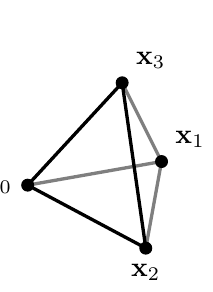
\begin{tikzpicture}
	\useasboundingbox (-1,-1) rectangle (1,2); 
	\draw (-1,0) node[fill, draw, circle ,minimum size=1.5mm,inner sep=0pt,outer sep=0pt, label=left:$\vec{x}_0$](p0){};
	\draw (0.5,-0.8) node[fill, draw, circle ,minimum size=1.5mm,inner sep=0pt,outer sep=0pt, label=south:$\vec{x}_2$](p2){};
	\draw (0.7,0.3) node[fill, draw, circle ,minimum size=1.5mm,inner sep=0pt,outer sep=0pt, label=north east:$\vec{x}_1$](p1){};
	\draw (0.2,1.3) node[fill, draw, circle ,minimum size=1.5mm,inner sep=0pt,outer sep=0pt, label=north east:$\vec{x}_3$](p3){};
	\draw[line width=1.2pt, -] (-1,0) -- (0.5,-0.8);
	\draw[line width=1.2pt, -, opacity=0.5] (-1,0) -- (0.7,0.3);
	\draw[line width=1.2pt, opacity=0.5] (0.5,-0.8) -- (0.7,0.3);
	\draw[line width=1.2pt, -] (-1,0) -- (0.2,1.3);
	\draw[line width=1.2pt] (0.2,1.3) -- (0.5,-0.8);
	\draw[line width=1.2pt, opacity=0.5] (0.2,1.3) -- (0.7,0.3);
	\end{tikzpicture}	
	\caption{A sample tetrahedral element, with 4 vertices at positions $\vec{x}_0$, $\vec{x}_1$, $\vec{x}_2$, and
		$\vec{x}_3$.}
	\label{fig:f2}
\end{figure}

To solve the problem of volumetric locking, instead of enforcing a per-tetrahedron
near-incompressibility with high Poisson's ratio, 
%we propose to enforce incompressibility through constraining volumes of zones defined as local sets of finite elements. Specifically, we add zonal volume constraints to the general energy minimization problem defined in equation~\eqref{eq:energy_min}. 
we adopt the approach of Mixed Finite Element Method as in \ref{eq:mixed_variational}. Essentially,
we solve the saddle-point system as a constrained minimization with constraint function
$\vec{c}(\vec{x}) = \vec{0}$. Specifically, our constraint enforces the total volumes of zones defined as
local sets of finite elements to be preserved.
Compared to other mixed elements, our approach is much more efficient and easier to implement while showing
comparable results. Moreover, our approach provides the modeling flexibility of choosing zones that 
are aligned with anatomical compartments (see Section~\ref{sec:zoning}).

Each constraint is simply formulated as the requirement that the total volume of all elements in a
specified zone of the deformed mesh is equal to the initial volume. That is, for $j$-th zone $G_j$, the zonal
volume constraint function $c_j$ is defined as follows,
\begin{equation}
c_j(\vec{x}) = \sum_{e \in \zeta_j} V_e(\vec{x}) - V_e^0,
\end{equation}
where $V_e^0$ is the reference volume of element $e$, which belongs to zone $j$ with element index set $\zeta_j$.

Imposing this constraint for each zone gives us a new constrained minimization problem:
\begin{align}
\min_{\vec{x}}\ & \int_{\Omega} \Psi(\vec{x}) \\
\text{s.t.}\ & c_j(\vec{x}) = 0 \quad \forall j.
\label{eq:constrained-min}
\end{align}
As a special case we can preserve the total volume with a single \emph{global} constraint; by
contrast, classical incompressible Neo-Hookean models require the volume of each and every element
to be preserved. 

To illustrate the simplicity of this type of constraint we define the volume constraint for a
tetrahedral mesh. The volume of the tetrahedron $e$, as depicted in Figure~\ref{fig:f2}, is defined
(up to a constant scaling) as the triple scalar product
\begin{align*}
V_e(\vec{x}) = \vec{v}_3 \cdot (\vec{v}_1 \times \vec{v}_2),
\end{align*}
where $\vec{v}_i = \vec{x}_i - \vec{x}_0$.  Then the Jacobian of the constraint function can be
computed as
\begin{align*}
\frac{\partial c_j}{\partial \vec{x}} = \sum_{e} \frac{\partial V_e}{\partial \vec{x}},
\end{align*}
where the sparse vector $\frac{\partial V_e}{\partial \vec{x}} \in \R^{3n}$ is zero everywhere
except for the vertices of element $e$, where
\begin{align*}
\left[\frac{\partial V_e}{\partial \vec{x}}\right]_0 = 
-(\vec{v}_2 \times \vec{v}_3 + \vec{v}_3 \times \vec{v}_1 + \vec{v}_1 \times
\vec{v}_2)
\end{align*}\begin{align*}
\left[\frac{\partial V_e}{\partial \vec{x}}\right]_1 = \vec{v}_2 \times \vec{v}_3, \quad
\left[\frac{\partial V_e}{\partial \vec{x}}\right]_2 = \vec{v}_3 \times \vec{v}_1, \quad
\left[\frac{\partial V_e}{\partial \vec{x}}\right]_3 = \vec{v}_1 \times \vec{v}_2.
\end{align*}

%\begin{figure}[t]
%  \centering
%  \begin{subfigure}{.49\linewidth}
%    \centering
%    \includegraphics[width=1.0\textwidth]{images/medpuck_049_50.png}
%    \caption*{(a)}
%    \label{sfig:medpuck_049_50}
%  \end{subfigure}%
%  \begin{subfigure}{.49\linewidth}
%    \centering
%    \includegraphics[width=1.0\textwidth]{images/medpuck_049_vcip_50.png}
%    \caption*{(b)}
%    \label{sfig:medpuck_049_vcip_50}
%  \end{subfigure}\par\medskip
%  \begin{subfigure}{.49\linewidth}
%    \centering
%    \includegraphics[width=1.0\textwidth]{images/puck_049_vcip.png}
%    \caption*{(b)}
%    \label{sfig:puck_049_vcip_50}
%  \end{subfigure}%
%  \begin{subfigure}{.49\linewidth}
%    \centering
%    \includegraphics[width=1.0\textwidth]{images/puck_0475_vcip_50.png}
%    \caption*{(d)}
%    \label{sfig:puck_0475_vcip_50}
%  \end{subfigure}%
%  \caption{\textbf{Reproducing High-Res Simulations}: (a) is a high-resolution puck with 180K
%    tetrahedrons with $\nu = 0.49$ without a zonal volume constraint. (b) is the result with a global
%    volume constraint with the same Poisson's ratio $\nu = 0.49$. (c) shows a low-res simulation
%    with global volume constraint with the Poisson's ratio $\nu = 0.49$, (d) is a lower resolution
%    22K tetrahedrons with our method with $\nu = 0.475$ that recreates the high-resolution results
%    (a) and (b) closely. \todo{remove example and replace with some other case where low-res recreates hi-res}}
%  \label{fig:res_compare}
%\end{figure}
%\todo{fig:res_compare parts c and d. not clear what you are trying to say}
Finally, the Hessian stencils for each $V_e$ will be simple linear skew-symmetric matrices.
% DKP: this needs elaboration that elements are linear in the
% vertex positions. For now, let's save that for another day, since we
% don't exploit it yet.
Thus, $c_{j}(\vec{x}) = 0$ is a one dimensional constraint with simple to implement sparse
derivatives, which gives true volume preservation.
% imcompressibility with respect to the surface of the solid
Note that this constraint can be further optimized by computing the volume of the entire zone by
iterating over zone boundary faces only.

Although uncomplicated, this constraint provides a powerful tool for emulating incompressible
elasticity. It allows users to achieve volume preservation without increasing Poisson's ratio,
which can cause instabilities and locking. For most nonlinear solvers a few equality constraints should not be prohibitively expensive to solve, but for additional performance gain one may naturally use an Augmented Lagrangian method to solve the constraints. 

The zone sizes are important in determining the level of local incompressibility. One global zone
for the entire mesh will essentially be a hydrostatic simulation, analogous to simulating a water
balloon. As the zone sizes decrease, there will be more local incompressibility around each element
which will result in a stiffer behavior. However, as long as the zones are at least as large as the
1-ring \cite{Irving:2007}, volumetric locking will not occur. Therefore, as we use a smaller zone
sizing, the results will become more similar to the results in \cite{Irving:2007}, but at a steeper performance cost. 

Our method can be viewed as a simplification of the 2-field mixed
formulation~\eqref{eq:mixed_variational}, where the pressure potential is given as
\begin{equation}
\vec{p}^{T}\vec{c}(\vec{x}) = \sum_j \vec{p}_j c_j(\vec{x}) = \sum_j \vec{p}_j \left( \sum_{e \in G_j}
V_e(\vec{x}) - V_e^0 \right),
\label{eq:variational_lagrange}
\end{equation}
where the interpolated hydrostatic pressures $\vec{p}_j$ for zone $j$ are identified to be the
Lagrange multipliers for the $j$-th zonal volume constraint. If each element was assigned to a unique
zone, our method would recreate the mixed-element formulation for incompressible materials. However,
we use only a handful of zones, which keeps the problem size small and avoids locking and instability.

\new{
	An important advantage of enforcing volume preservation with zonal constraints is that it allows a way of simulating incompressible
	objects using a much coarser mesh than by using a traditional 1-field method. C\'ea's lemma already couples the quasi-best approximation error 
	with mesh resolution, and since a 1-field FE solutions also couple the bulk modulus to the upper bound of the approximation error, it makes it 
	even harder to use a coarser mesh when bulk modulus is high. However, when incompressibility is decoupled from the bulk modulus, and we can 
	use much smaller $\lambda$, we are able to achieve simulation results of a fine-mesh simulation that is consistent with a much coarser mesh. 
	Figure~\ref{fig:fine-ball} shows a simple dynamic simulation with a very fine mesh, and Figure~\ref{fig:coarse-ball} shows the same simulation
	using a much coarser mesh. We see that both the low Poisson ratio and our method achieves consistent visual results between the fine and coarse
	case, but the high Poisson ratio case fails to converge very early in the simulation.
}

\new{
	We solved the constraints using Ipopt \cite{Wachter:2006}, a non-linear optimization package based on interior point method.
	However, our method should work with any non-linear optimizer that is able to deal with nonlinear equality constraints. 
	In our experiments, we found that not much parameter tuning was required to use our method with Ipopt: we only occasionally had to tune the \texttt{nlp_scaling_max_gradient} parameter when used with additional nonlinear constraints. 
}
\todo{additional explanation on Ipopt?}

\subsection{Stabilization}
We apply the F-bar method \cite{neto:2005} to the energy density function to ensure stability. 
This is based on a multiplicative split of the deformation gradient $\vec{F}$ into 
a deviatoric and volumetric component. The deviatoric part is computed as
\begin{equation}
\bar{\vec{F}}= \alpha \vec{F},
\label{eq:F-bar}
\end{equation}
where
\begin{equation}
\alpha = \frac{\bar{J}^{\frac{1}{3}}}{J^{\frac{1}{3}}},
\label{eq:F-bar_alpha}
\end{equation}
and $\bar{J}$ is the average of $J$ computed over a set of local element stencils. In our case, the
local setss are the zones where the total volume is preserved, hence conveniently 
$\bar{J} = 1$, and $\alpha = J^{-\frac{1}{3}}$. However, since as $J \rightarrow 0$ we have that $\alpha \rightarrow +\inf$, we instead apply a C-2 extension to $\alpha$ below a certain threshold $\epsilon$, similarly to \cite{Stomakhin:2012}. Then the new extended deviatoric projector is given as
\begin{align}
\tilde{\alpha} := 
\begin{cases}
\begin{array}{l} J^{-\frac{1}{3}} \end{array}  & \text{for } J > \epsilon\\
\begin{array}{l@{}l}
\epsilon^{-\frac{1}{3}} &\,-\, \frac{1}{3} \epsilon^{-\frac{4}{3}} (J - \epsilon)
\,+\, \frac{2}{9} \epsilon^{-\frac{7}{3}} (J - \epsilon)^2
\end{array} & \text{for } J \leq \epsilon
\end{cases}
\label{eq:c2}
\end{align}
In practice, the choice of $\epsilon$ is not too important as long as it is small ($\sim 0.1$). 

We then use $\bar{\vec{F}}(\vec{x})$ to compute the deviatoric part of the constitutive equation. For example, 
the deviatoric part of Neo-Hookean energy density function \eqref{eq:neohookean} will now be computed as
\begin{align}
\bar{\Psi}_{\text{NH}}(\vec{\bar{\vec{F}}}; \lambda, \mu) = \frac{\mu}{2}(\tilde{\alpha}^2 I_C - 3).
\label{eq:deviatoric_neohookean}
\end{align}
Note that this is similar to the form presented by Rivlin \shortcite{Rivlin:1948}, but extended below 
$\epsilon$ to be continuously defined for $J \leq \epsilon$. 

Using only the deviatoric component of deformation gradient for the elastic potential energy, we remove the contribution of the constitutive equation on the pressure. Hence, this allows the complete split of the total elastic stress, to the deviatoric stress from the elastic potential, and the volumetric stress from the constraint Lagrange multipliers and the volume penalty.
\chapter{Volume Penalty}
\label{ch:Volume Penalty}

Our method ensures that volume is preserved within each zone, but without any element-wise volume
change penalty the volume inside each zone can transfer between elements. This is a feature, as discussed in the Introduction, since
it reduces the cost and numerical challenges of enforcing volume preservation locally, while
ensuring good behavior globally.  Note that, unlike in the hydrostatic case, volume can not transfer
completely freely since elastic forces due to the shear modulus restrict large flows. 


However, the zonal constraints by themselves model only the hydrostatic pressure in the coarse zones, hence we also need to model the finer-scale pressures in the individual elements.
We employ a more traditional approach to modeling element-wise pressure in the penalty method.
To model this local compression penalty function, we look at the volume penalty functions present in various Neo-Hookean elasticity models.
In Neo-Hookean models, the bulk modulus models how much the material resists element-wise volumetric deformation. 
The bulk moudulus is represented in most Neo-Hookean energy formulations in the first Lam\'e parameter $\lambda$, which is a combination of the shear and bulk modulus.
However, as discussed in Section~\ref{ch:Background}, when $\lambda \rightarrow +\infty$ locking occurs, and the pressure computations become unstable.
But since we model the coarse-scale pressures as constraints, and we only need to model the finer-scale deviations in pressures, we are able to use a lower $\lambda$ and avoid locking.


If $\lambda$ is set too low the simulation is more susceptible to collapsing elements 
and even equilibrium configurations with inverted elements for invertible energy models.
Consider the example in Figure~\ref{fig:pucks} of a cylindrical puck with a moving Dirichlet
boundary condition on a set of vertices on top of the puck. As the puck compresses, the tetrahedra
underneath the moving boundary are flattened to the point where subsequent steps cause boundary
adjacent tetrahedra to invert. At this point, incompressible energy models with a logarithmic volume
penalty ($\log J$) term will become undefined because $J \leq 0$. Other models, like co-rotated
elasticity, may permit inverted elements, but won't be able to recover from an inverted
configuration. This issue has motivated a number of solutions \cite{Irving:2004,Smith:2018} for
handling inverted elements, but we will focus on the recent work on the Stable Neo-Hookean
model developed by Smith et al. While the proposed model attempts to solve many of the issues with
non-invertible energies and doesn't require additional parameters, as can be seen from the plot
of the volume change penalty term in terms of relative volume change $J$ in Figure~\ref{fig:penalty_plots},
the Stable Neo-Hookean energy resists compression much more timidly as compared to
the standard Neo-Hookean model defined in Equation \eqref{eq:neohookean}.

This results in the simulation possibly converging to an invalid configuration where inverted elements exist, 
and a nonlinear optimization solver can struggle due to inverted elements being present in intermediate solutions which cause oscillations.
Especially, this oscillation can be aggravated when constraints are introduced, presenting major performance issues when one tries to use volume constraints. 

%% TODO with new energy model
\begin{figure}[t] 
	\centering
	\begin{subfigure}{.49\linewidth}
		\centering 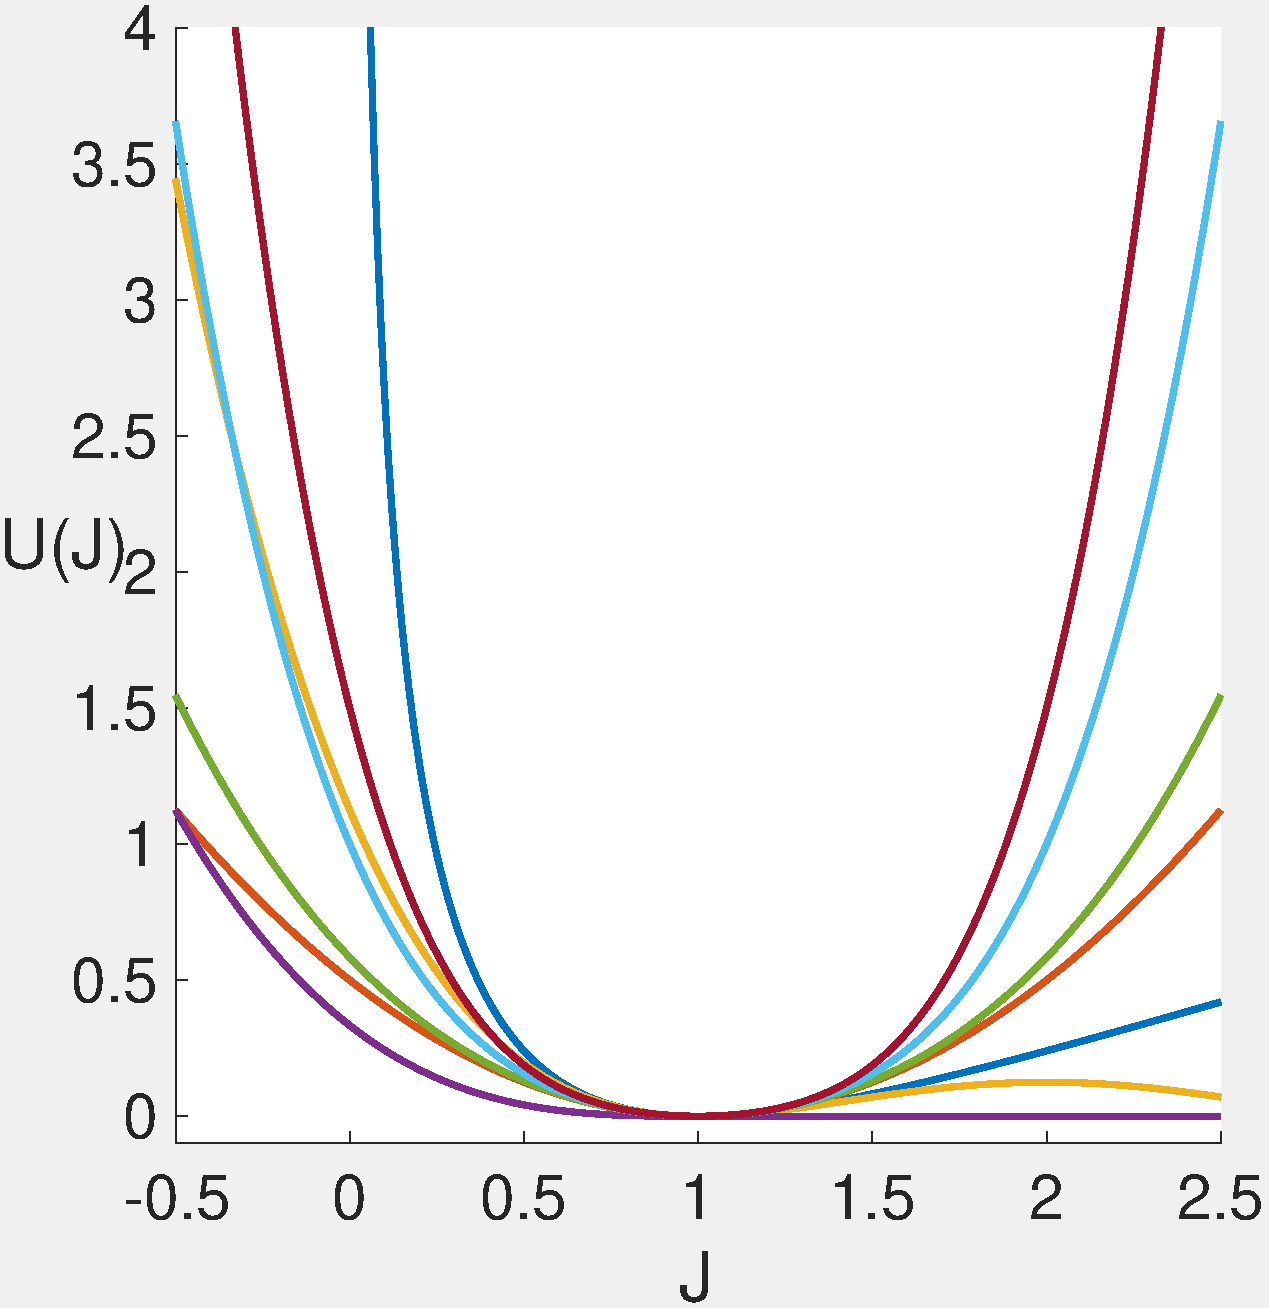
\includegraphics[width=2.0in]{images/pen_plot.pdf}
		\caption*{(a)}
		\label{sfig:energy_plot}
	\end{subfigure}%
	\begin{subfigure}{.49\linewidth}
		\centering 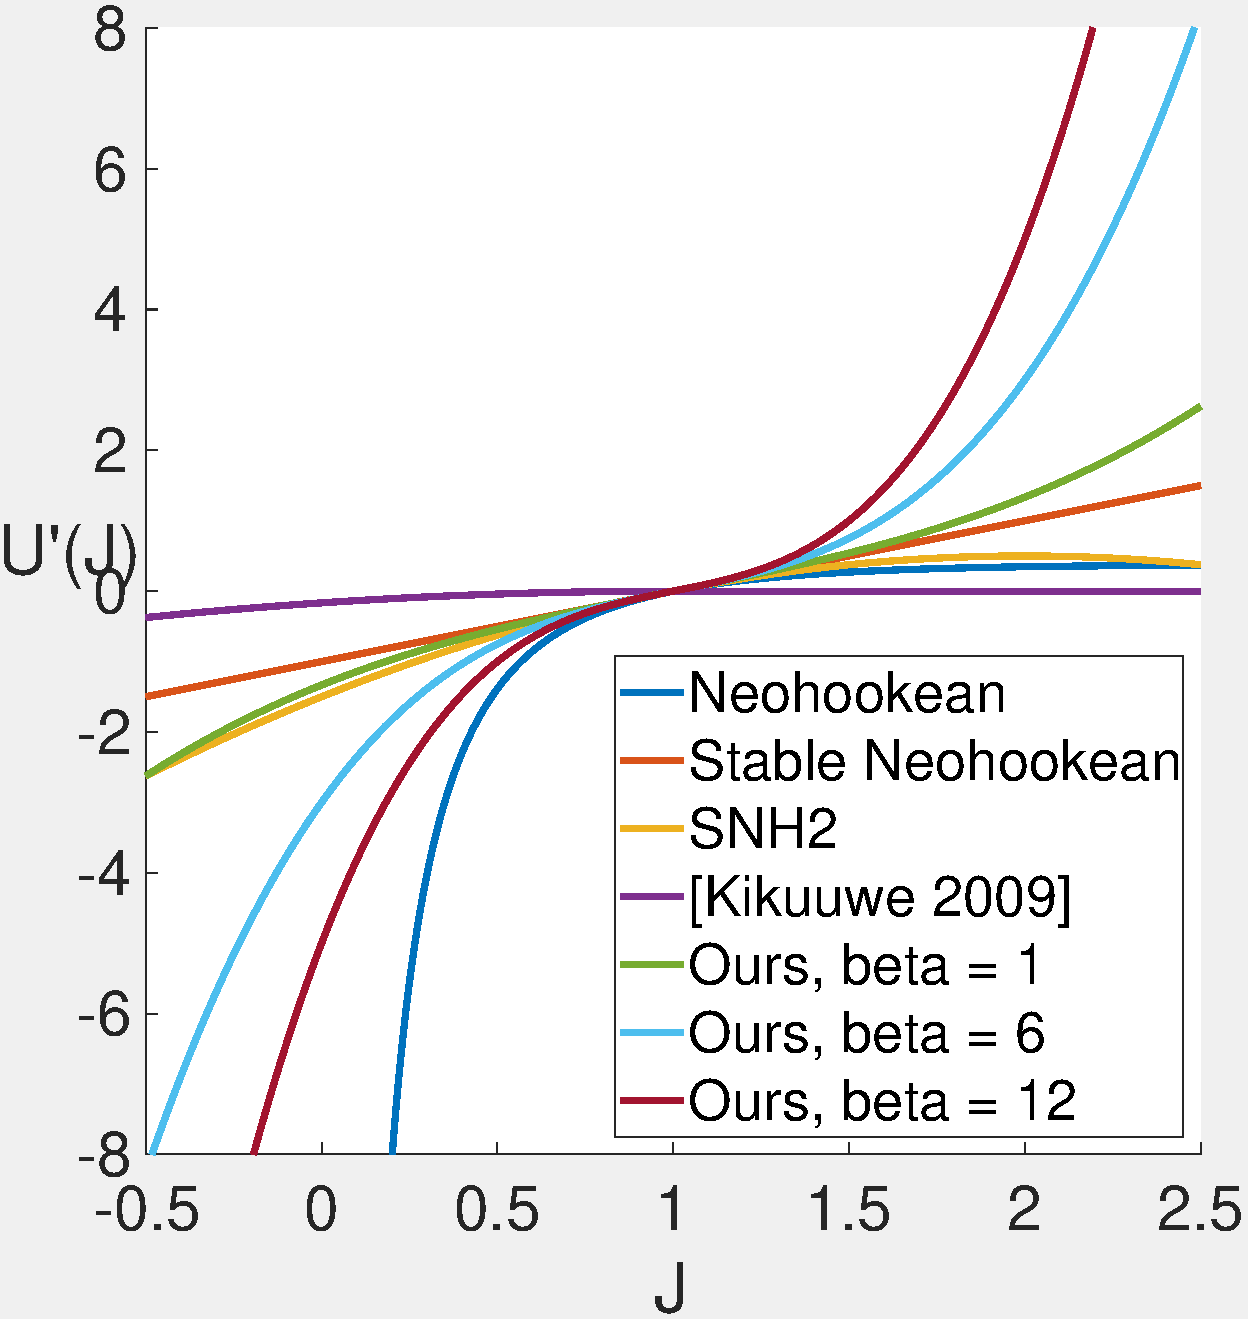
\includegraphics[width=2.0in]{images/stress_plot.pdf}
		\caption*{(b)}
		\label{sfig:stress_plot}
	\end{subfigure}%
	\caption{\textbf{Penalty Plots}: A plot of the penalty terms $U(J)$ and their stresses $U'(J)$ from different
		energy formulations (Neo-Hookean, Stable Neo-Hookean \cite{Smith:2018}, the second-order expanded version of Stable Neo-hookean, \cite{kikuuwe:2009},
		ours with $\beta=1$, and ours with $\beta=6$) with $\lambda = 1$, in terms of the relative volume change $J$. 
		The Neo-Hookean volume term (blue) indicates a substantially larger penalty
		when compared to Stable Neo-Hookean (orange) 
		and \cite{kikuuwe:2009} (yellow), but the penalty term is undefined when $J \leq 0$ due to its log term.
		This is more evident to see in the stress plot during compression ($J < 1$), where the Stable
		Neo-Hookean volumetric stress changes in a linear manner. Our method for both $\beta=1$ (purple) and $\beta=6$ (green) shows much more effective penalization under compression and stretch. Our stresses shows a nonlinear dependence on $J$
		similar to the Neo-Hookean term, but also shows a effective growth not only during compression but also during stretch. }
	\label{fig:penalty_plots}
\end{figure}

This suggests a need for a good penalty term that is both invertible and still resists compression
effectively. Let us write such penalty term as $U(J)$, controlled linearly by parameter $\lambda$.
To design such a penalty term, we first take a look at what conditions the function $U(J)$ must
meet. 

A detailed study of various Neo-Hookean compression penalty terms and explanations for each of the 
conditions can be found in \cite{hartmann:2003}.

\begin{enumerate}[label=\alph*)]
	\item The function must evaluate to 0 at rest ($J = 1$).
	\item The gradient of the function, i.e the volumetric stress, must also evaluate to 0 at rest.
	\item For the $\lambda$ of the penalty term to  correspond to the Lam\'e parameter in linear elasticity, $\frac{\partial^2 U(1)}{\partial J^2} = 1$ must hold.
	\item The function must be defined for all real numbers $(-\infty, +\infty)$.
	\item $\frac{\partial^2 U(J)}{\partial J^2} \geq 0, \,\forall J \in \R$ for the penalty to both penalize compression and stretch.
\end{enumerate}

Consider the following function,
\begin{equation}
U(J; \beta) := \frac{1}{12} (J-1)^2 \left[ \beta (J-1)^2 + 6 \right],
\label{eq:penalty_function}
\end{equation}
where the parameter $\beta \in [0, +\infty)$ controls how steeply the penalty function will penalize change in $J$. 
The first and second derivatives of the function are 
\begin{align}
\frac{\partial U(J; \beta)}{\partial J} &= \frac{1}{3} (J-1) \left[ \beta (J-1)^2 + 3 \right], \text{ and}\\
\frac{\partial^2 U(J; \beta)}{\partial J^2} &= \beta (J-1)^2 + 1. 
\label{eq:penalty_derivatives}
\end{align}
Therefore, the function satisfies all of the conditions listed above.    
Note that for $\beta = 0$, $U(J;0) = U_{\text{SNH}}(J) = \frac{1}{2} (J-1)^2$. 
As $\beta$ is increases, the penalty function penalizes compression and stretch more effectively than the Stable
Neo-Hookean penalty term, while still being fully invertible. 
Therefore, this is a suitable choice for our compression penalty term.
Plots comparing different penalty terms $U(J)$ and stresses $\frac{\partial U(J)}{\partial J}$ are shown in Figure~\ref{fig:penalty_plots}.
Experimentally, $\beta = 1$ was sufficient for most realistic examples governed by external force, but for examples where inversions were more likely due to contact or boundary conditions, we could easily find higher $\beta$ that resolves all inversions.

The additional nonlinearity introduced in the gradient (Equation \eqref{eq:penalty_derivatives}) of our penalty function compared to a standard Stable Neo-Hookean penalty is the main reason for the inversion-robustness in our model. 
It is possible to formulate models with even higher nonlinearity than what we propose here, but in our
experiments we found that such energy models provide no significant benefit in resolving inversions
compared to \eqref{eq:penalty_function} and only increase the number of nonlinear solver iterations
until convergence. We discuss this further in Appendix~\ref{ap: Penalty}.

We demonstrate that by this simple addition to the energy potential, we can obtain results similar to 
that of using mixed finite elements as in \cite{Irving:2007}, but with very few or even 
one global constraint. The results of Figure  \ref{fig:suspended-cubes} demonstrate
that with a penalty of about $\nu = 0.45$ and with just one global zone, the deformations are close to 
using a 1-ring constraint around each vertex. 

Also, we found that simply adding this additional nonlinearity to the energy resulted in faster performances in most examples when volume constraint was used, and even in many cases where there were no constraints. 
In Table~\ref{tab:performance}, we compare the performance results of using $\beta = 0$ (equivalent to SNH) and higher $\beta$.
\chapter{Volumetric Zoning}
\label{ch:Volumetric Zoning}

\begin{figure}[h] \centering
	\adjustbox{trim={.25\width} {.0\height} {.25\width} {.0\height},clip}%
	{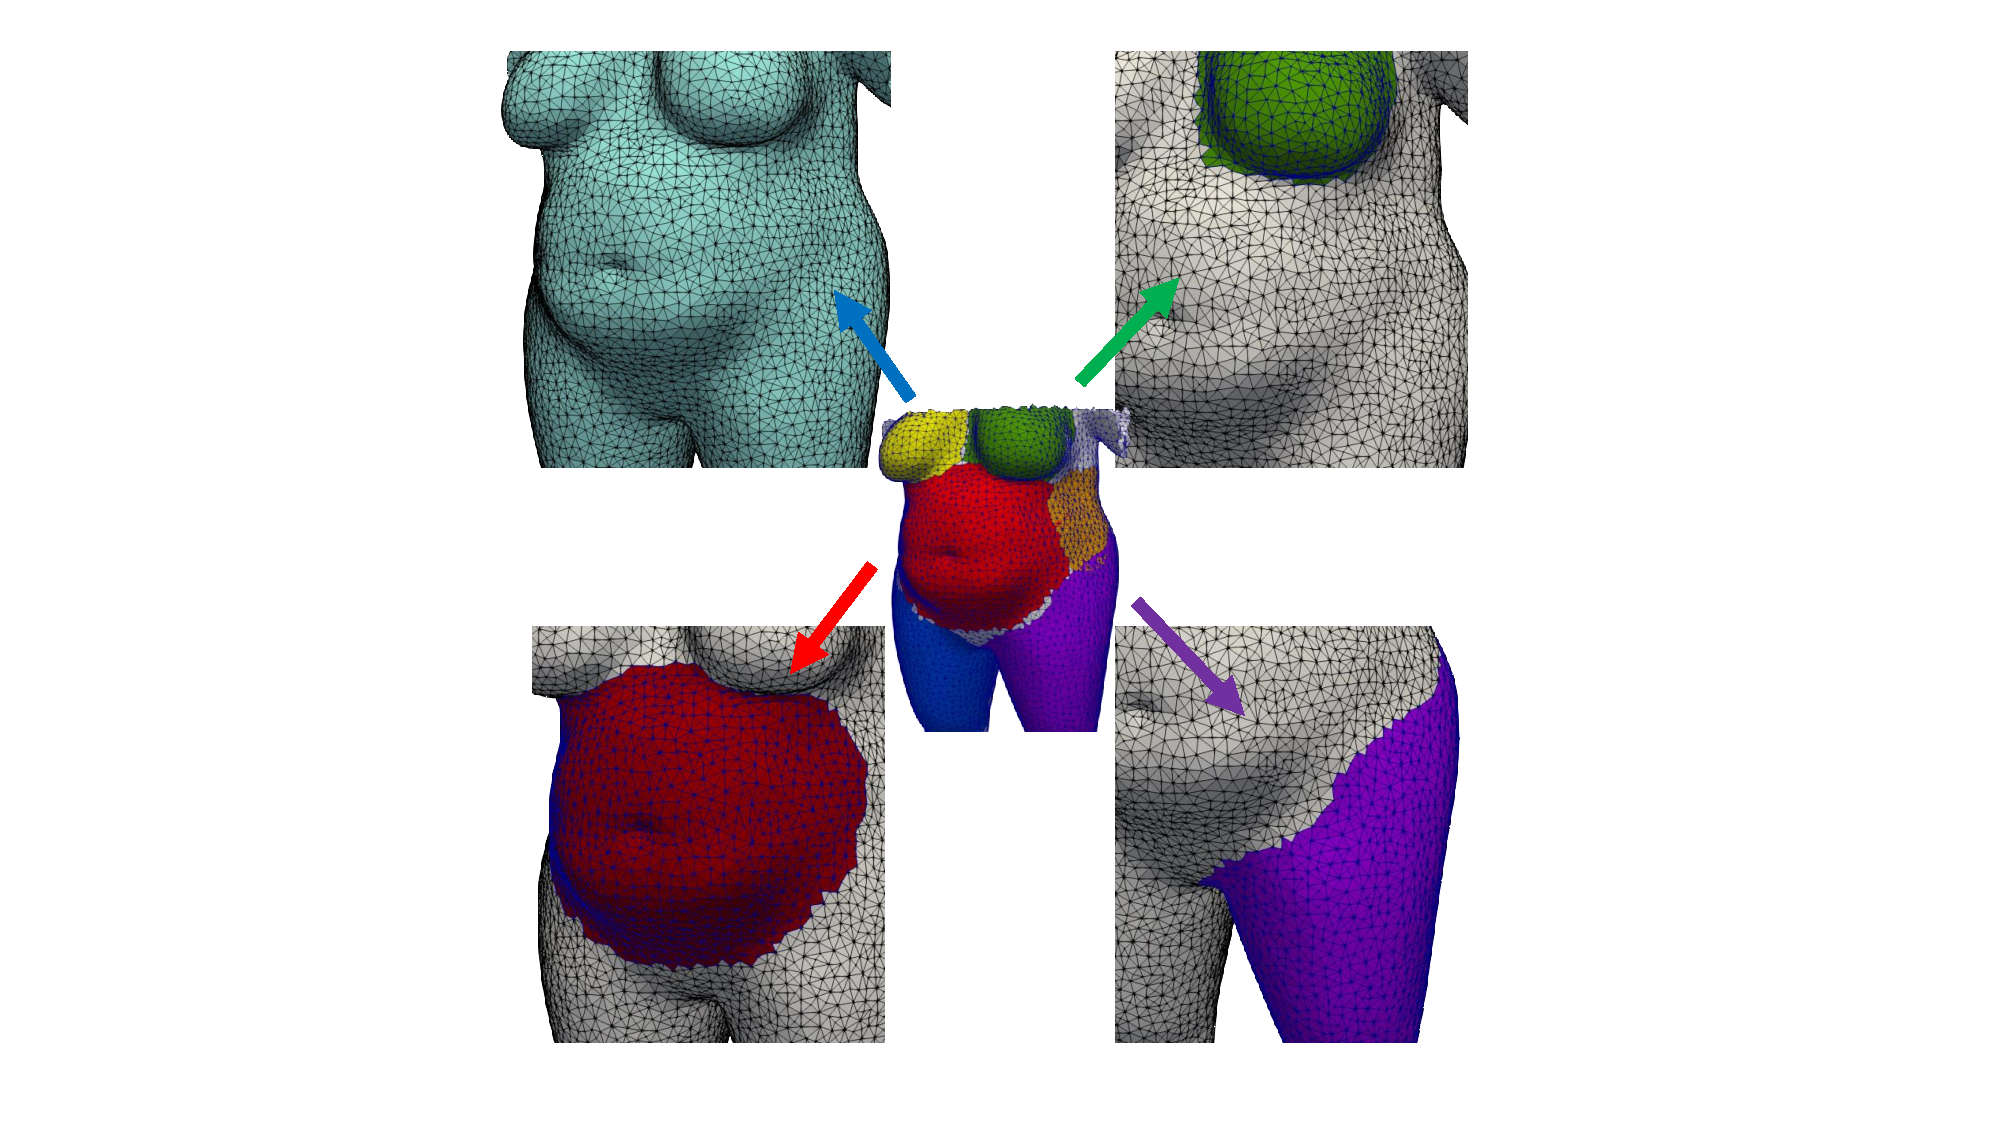
\includegraphics[width=6.0in]{images/body_xl/zones.pdf}}
	\caption{\textbf{Body Zones}: Volume preserving zones on the body mesh used for simulation in
		Figure~\ref{fig:teaser}. Six significant anatomical compartments (belly (red), side and back waist (orange), 2 legs (blue and purple), 2 breasts (yellow and green)) are selected as zones. Additionally, another zone is added including the full body (cyan), so that the entire body would be volume preserving. Note that the full body zone is not necessary, but can be added to ensure the volume preservation of not only each compartments but also the entire body. The zones are drawn on the mesh surface with a texture painting tool in a visual effects software, and then projected to the inner body using our projection method. }
	\label{fig:body_zones}
\end{figure}

For a more complete description of the pipeline, we propose a simple method of obtaining
volumetric zones on a tetrahedral mesh from surface vertex annotation.

Manual vertex painting is a very common part of
many character animation pipelines, allowing users to assign attributes such as skinning weights.
Alternatively, there are methods to automatically compute transformation weights from
skeleton meshes \cite{Rohmer:2009, Baran:2007, Weber:2007}, from sparse subsets of degrees of freedom
\cite{Jacobson:2012}, or from animation data \cite{James:2005}. 

Using either of the aforementioned methods, we end up with a set of weights defining possibly
overlapping zones on the surface of our FEM mesh. We then transfer this data onto the surface
triangles. Naturally these surface zones should be simply connected in order for the volumetric
zones to follow suit.

In order to transfer zone information to the rest of the tetrahedral mesh, we first construct a
smooth potential field around the mesh surface using Hermite Radial Basis Functions
\cite{Pai:2018, Vaillant:2013, Macedo:2009, Wendland:2004}, although any signed distance field will
do.  We then project each tetrahedron centroid along the potential gradient onto the surface
triangles. The triangle zone information is then copied from the triangles, back to the
source tetrahedra.

Albeit simple, this projection is an effective method to map internal tetrahedral mesh elements to
surface triangles. This way, we allow the users to define volume preserving zones by simply
painting surface vertices with any existing tool. We demonstrate
this approach with an sample female body simulation mesh on Figure~\ref{fig:body_zones}, where the
surface zones are chosen manually to capture the anatomical volume-preserving regions. 
\chapter{Results}
\label{ch:Results}

The following results demonstrate the versatility of our method. 
We use a tetrahedral mesh discretization for all our simulations.

Our implementation relied on the Ipopt non-linear optimization package \cite{Wachter:2006} to solve the constrained optimization problem proposed in equation~\eqref{eq:constrained-min}.
In our experiments, we found that excessive parameter tuning was not required to use our method with Ipopt: only when used with additional nonlinear constraints, we  occasionally tuned the texttt{nlp_scaling_max_gradient} parameter. 

For all our examples except for Twist (Figure~\ref{fig:twist}), we started with $\beta = 1.0$ and increased to improve performance.
However, for just resolving inversions and numerical instability, $\beta = 1.0$ works well for all of those examples.

\section{Two Tetrahedrons}

As the most simple proof of concept example for the volume constraint, we design a mesh with two
tetrahedrons with equal volume joined together by a face as shown in Figure~\ref{fig:twotets}. We
then compress one of the tetrahedrons with a Dirichlet boundary condition to a plane, to see the
effects of the volume constraint. The energy model used is Neo-Hookean with $\nu = 0.495$. 

As expected, the example without the global volume constraint loses around $50\%$ of the volume,
since the deformation of the compressed tetrahedron does not affect its neighbor.
When a volume constraint is applied, the unconstrained tetrahedron inflates to twice the original
size, keeping the total volume constant. 


\section{Twist}

\begin{figure}
	\centering
	\begin{tabular}{l|ccc}
		& UNH & Penalty, $\beta = 9$ & CNH \\
		\midrule
		$\frac{\pi}{2}$ &
		\begin{subfigure}{.25\linewidth}
			\centering
			\adjustbox{trim={.2\width} {.00\height} {.2\width} {.00\height},clip}%
			{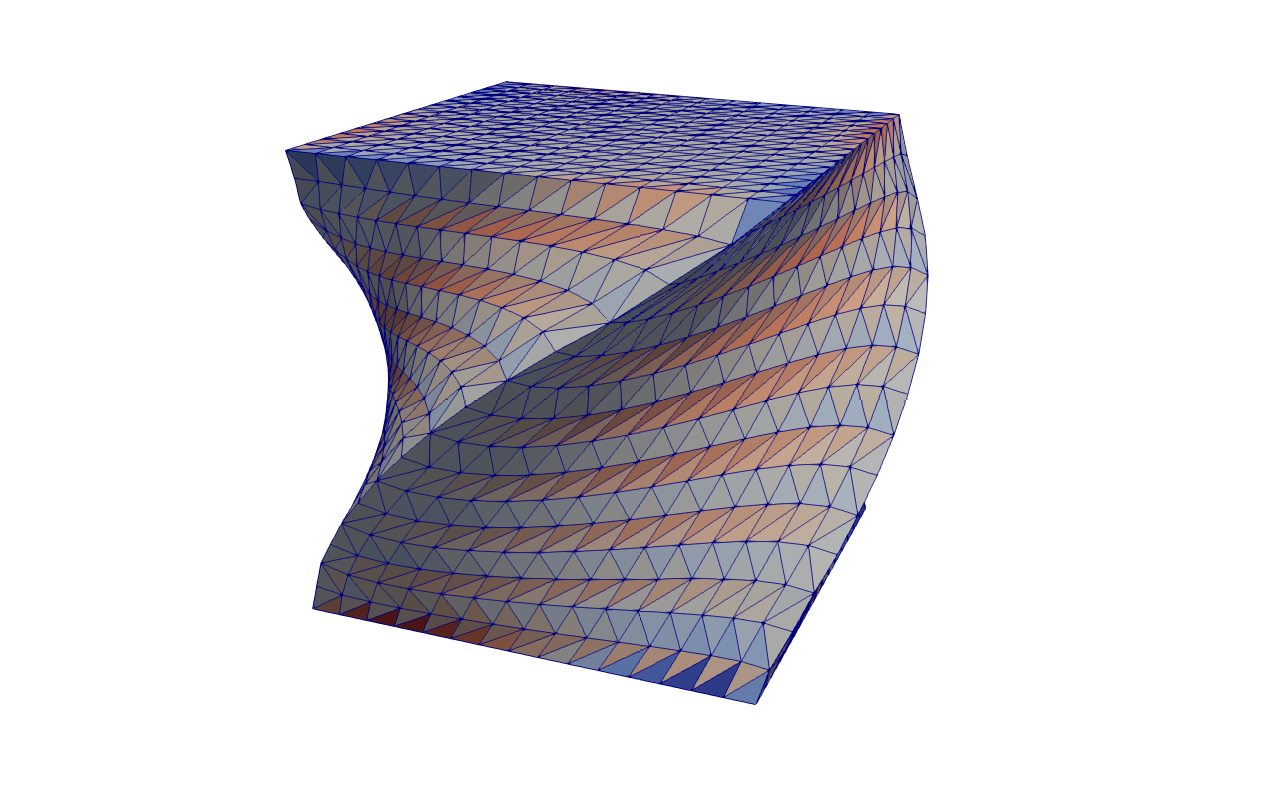
\includegraphics[width=2.0\textwidth]{images/twist/pr100-1.png}}
			%\caption*{(a1)}
			\label{sfig:twist-035-1}
		\end{subfigure} &
		\begin{subfigure}{.25\linewidth}
			\centering
			\adjustbox{trim={.2\width} {.00\height} {.2\width} {.00\height},clip}%
			{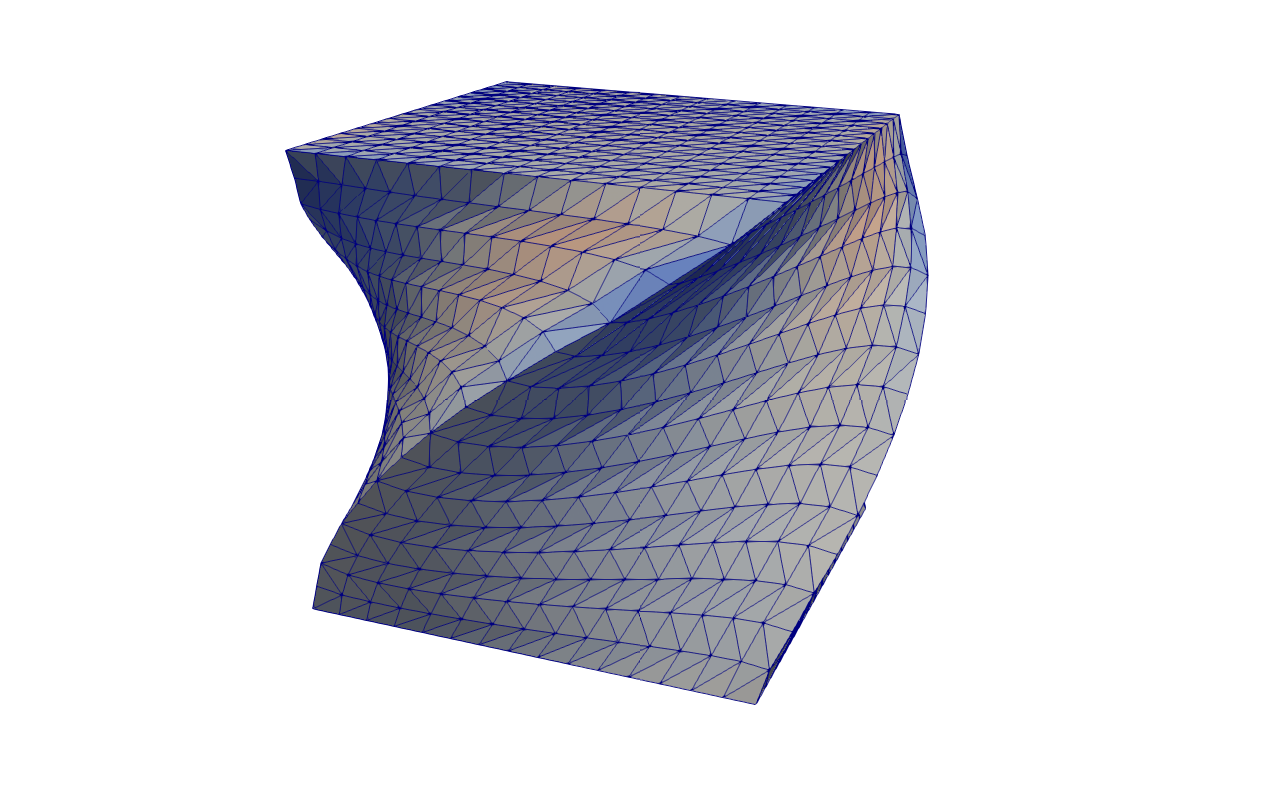
\includegraphics[width=2.0\textwidth]{images/twist/vp100-1.png}}
			%\caption*{(b1)}
			\label{sfig:twist-035-vc-1}
		\end{subfigure} &
		\begin{subfigure}{.25\linewidth}
			\centering
			\adjustbox{trim={.2\width} {.00\height} {.2\width} {.00\height},clip}%
			{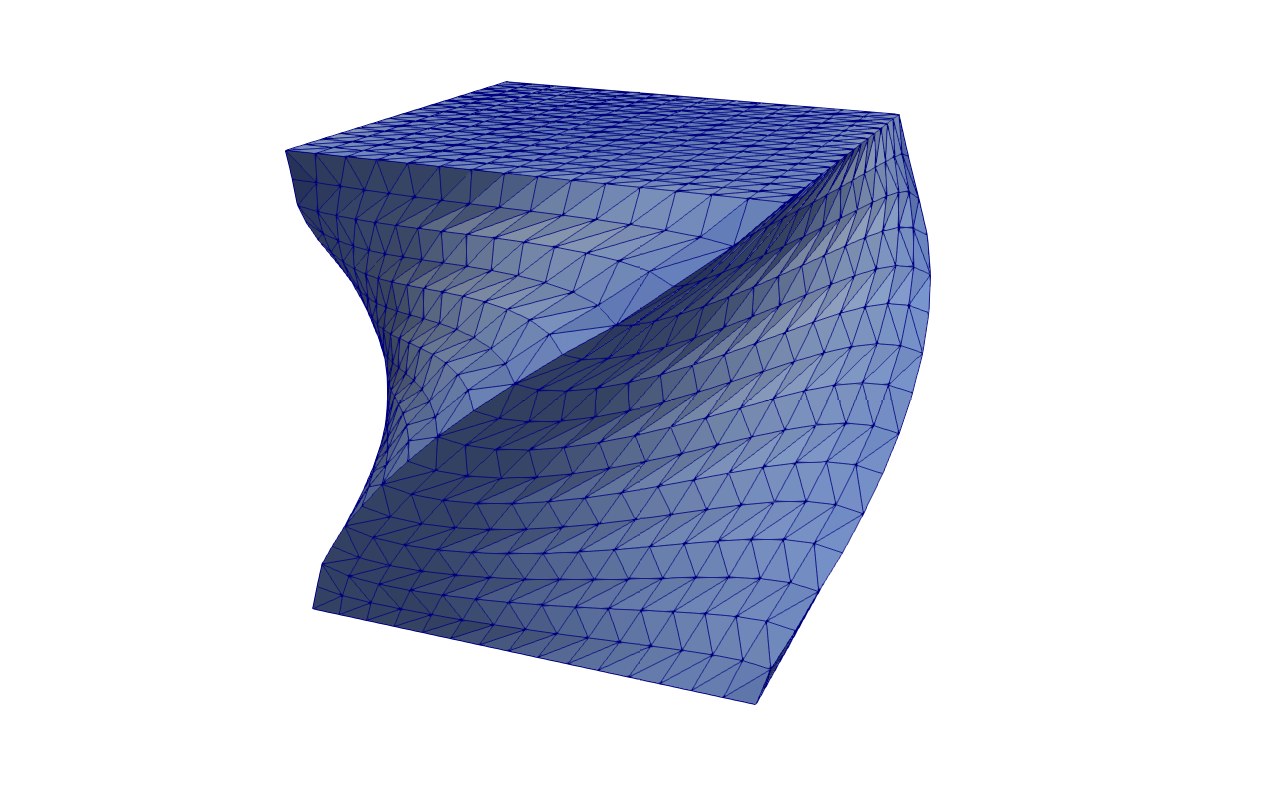
\includegraphics[width=2.0\textwidth]{images/twist/vc100-1.png}}
			%\caption*{(c1)}
			\label{sfig:twist-035-vcip-1}
		\end{subfigure}  \\
		$\pi$ &
		\begin{subfigure}{.25\linewidth}
			\centering
			\adjustbox{trim={.2\width} {.00\height} {.2\width} {.00\height},clip}%
			{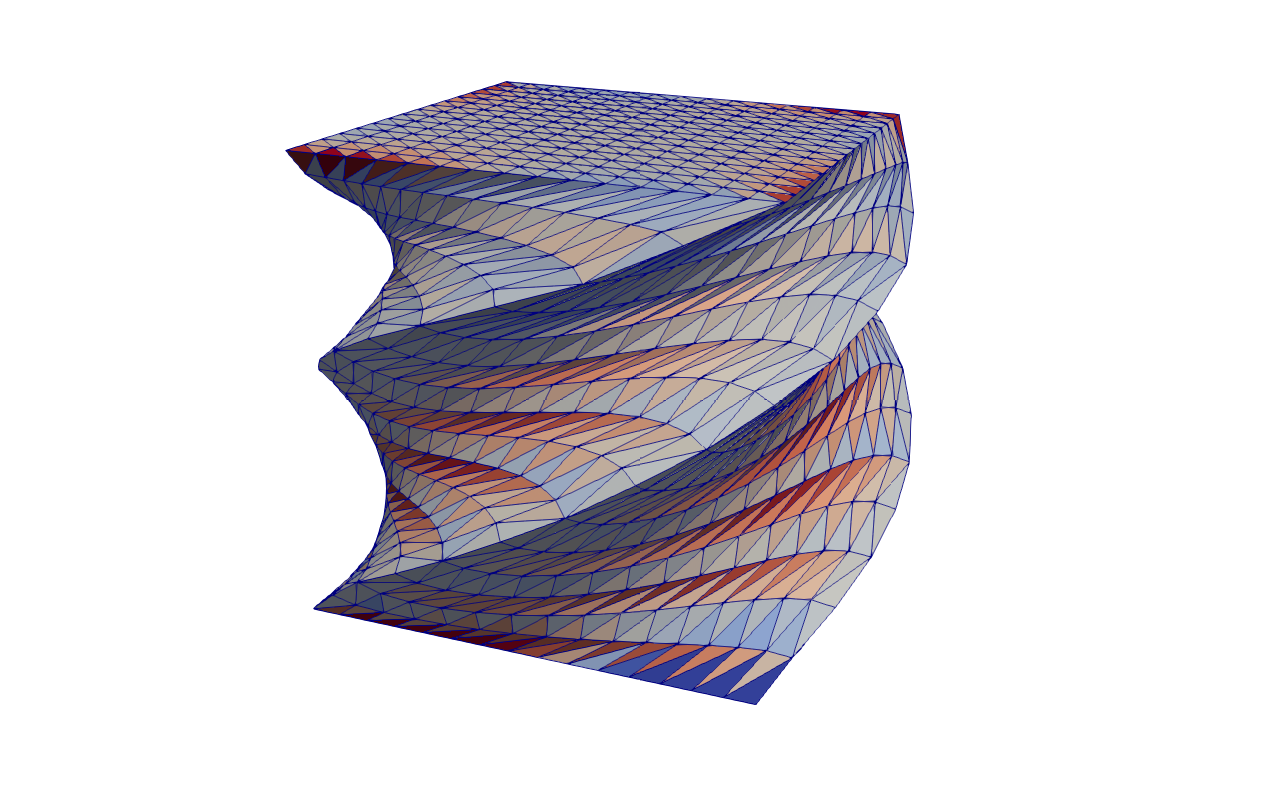
\includegraphics[width=2.0\textwidth]{images/twist/pr100-2.png}}
			%\caption*{(a2)}
			\label{sfig:twist-035-2}
		\end{subfigure} &
		\begin{subfigure}{.25\linewidth}
			\centering
			\adjustbox{trim={.2\width} {.00\height} {.2\width} {.00\height},clip}%
			{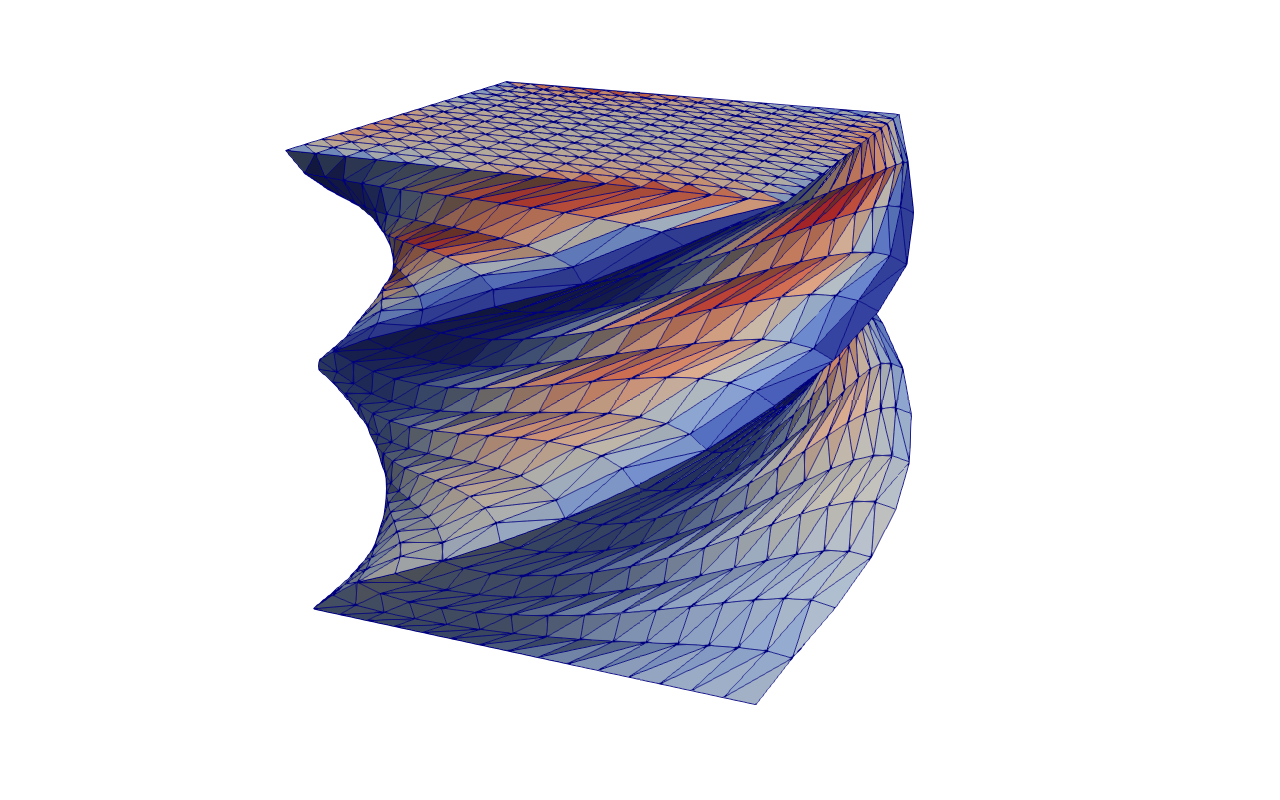
\includegraphics[width=2.0\textwidth]{images/twist/vp100-2.png}}
			%\caption*{(b2)}
			\label{sfig:twist-035-vc-2}
		\end{subfigure} &
		\begin{subfigure}{.25\linewidth}
			\centering
			\adjustbox{trim={.2\width} {.00\height} {.2\width} {.00\height},clip}%
			{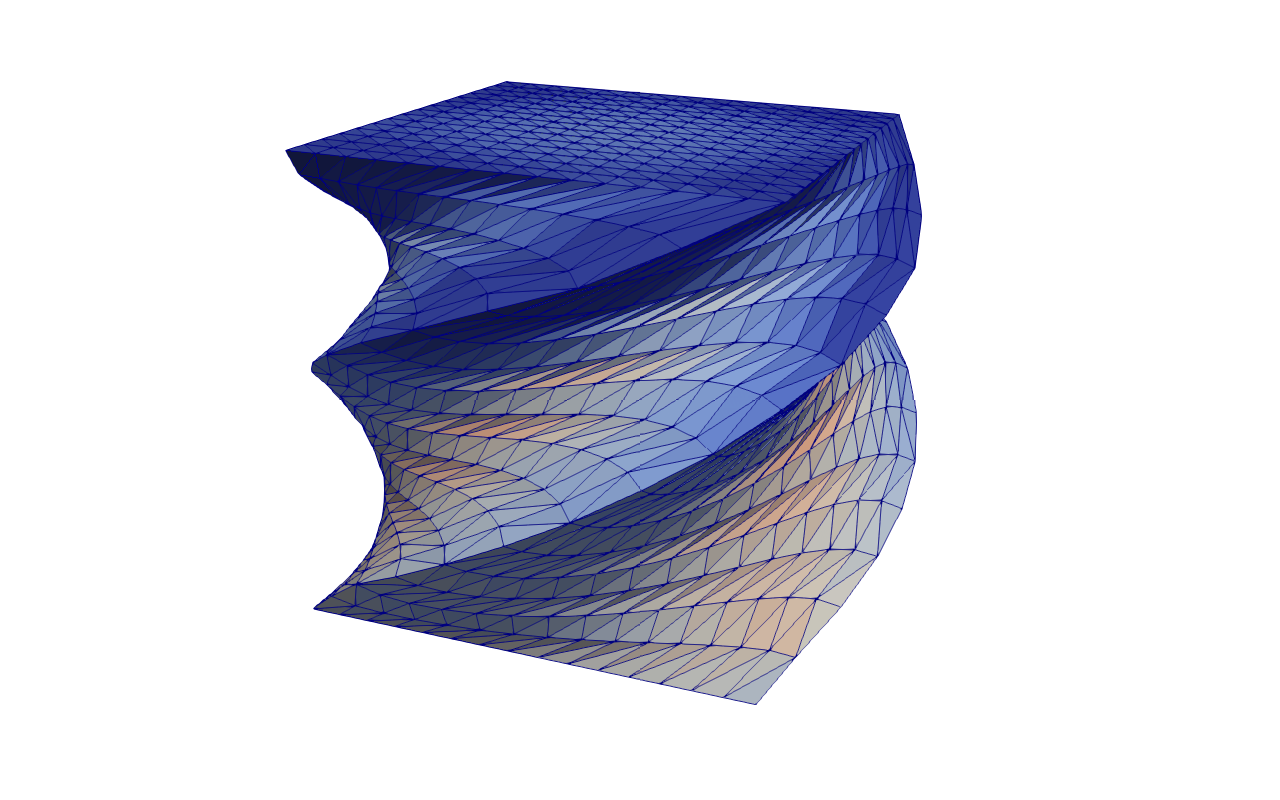
\includegraphics[width=2.0\textwidth]{images/twist/vc100-2.png}}
			%\caption*{(c2)}
			\label{sfig:twist-035-vcip-2}
		\end{subfigure} \\
		$\frac{\pi}{3}$ &
		\begin{subfigure}{.25\linewidth}
			\centering
			\adjustbox{trim={.2\width} {.00\height} {.2\width} {.00\height},clip}%
			{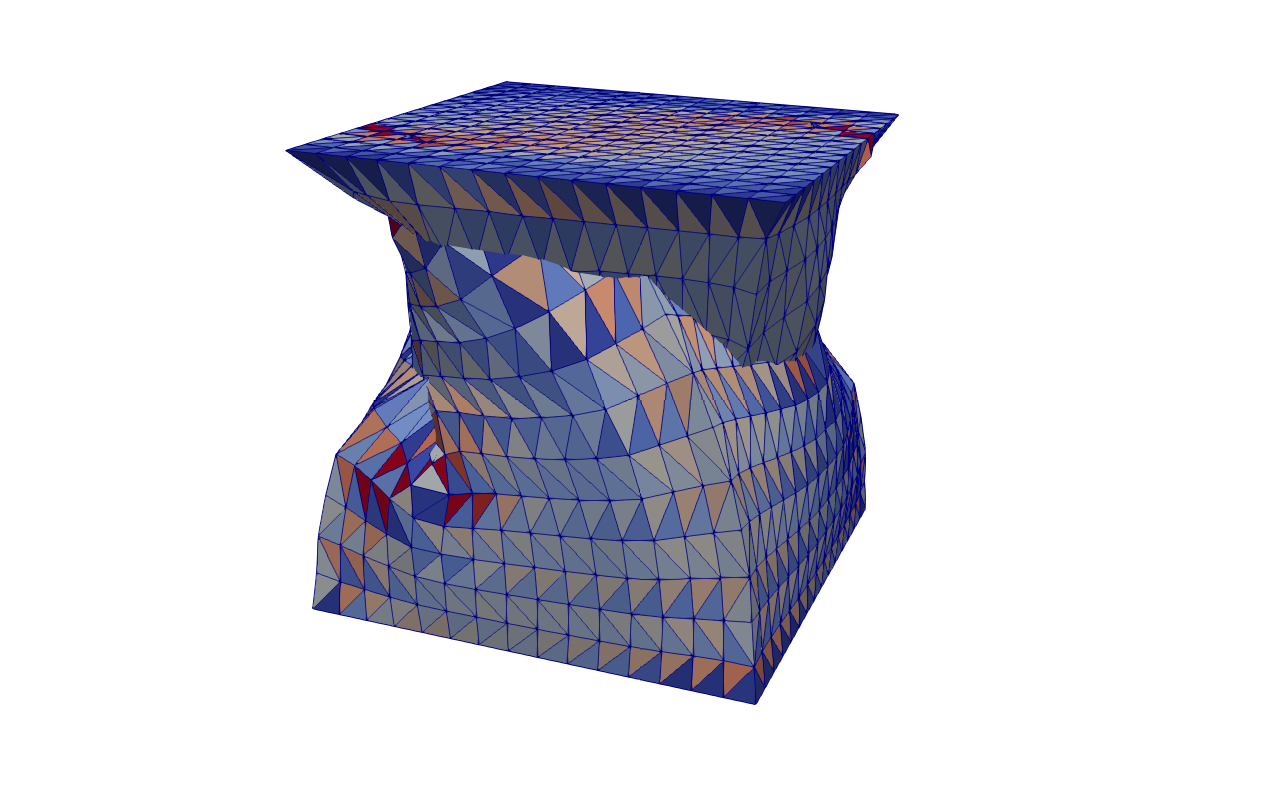
\includegraphics[width=2.0\textwidth]{images/twist/pr100-3.png}}
			\caption*{(a)}
			\label{sfig:twist-035-3}
		\end{subfigure} &
		\begin{subfigure}{.25\linewidth}
			\centering
			\adjustbox{trim={.2\width} {.00\height} {.2\width} {.00\height},clip}%
			{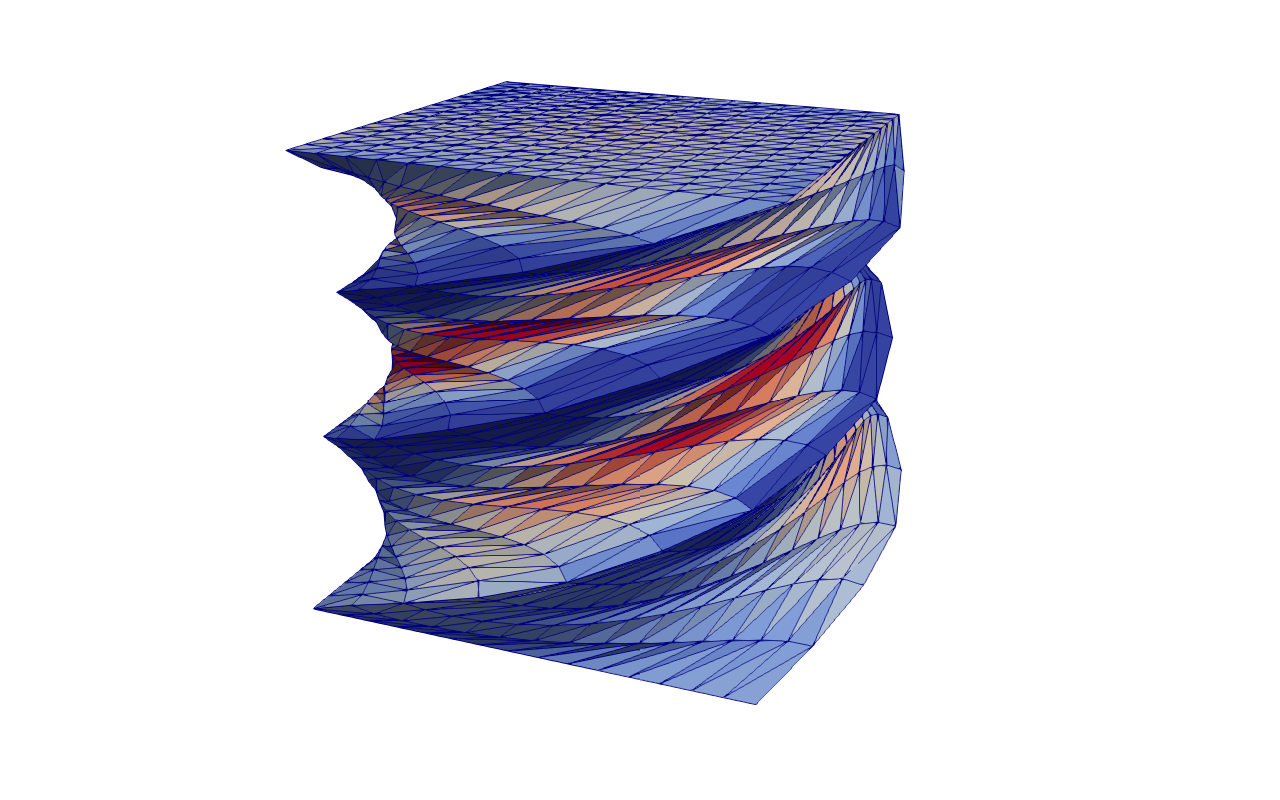
\includegraphics[width=2.0\textwidth]{images/twist/vp100-3.png}}
			\caption*{(b)}
			\label{sfig:twist-035-vc-3}
		\end{subfigure} &
		\begin{subfigure}{.25\linewidth}
			\centering
			\adjustbox{trim={.2\width} {.00\height} {.2\width} {.00\height},clip}%
			{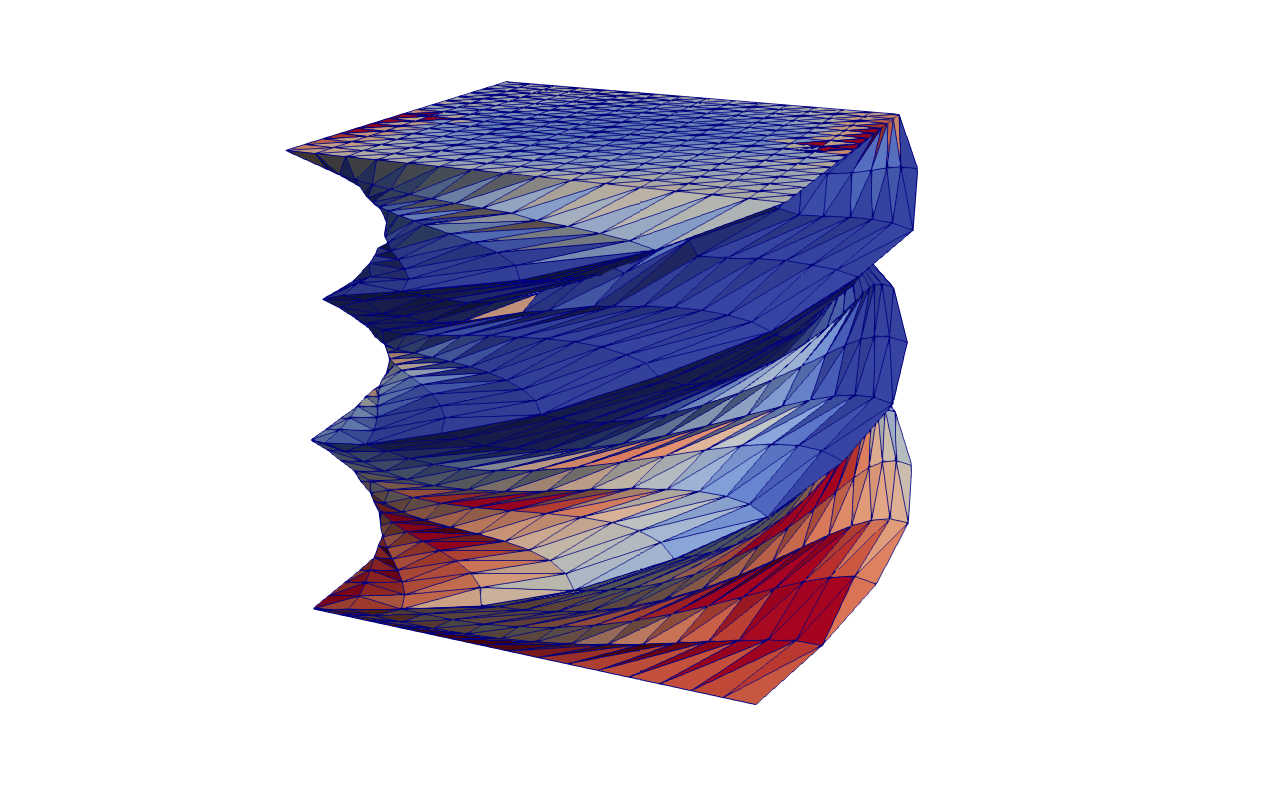
\includegraphics[width=2.0\textwidth]{images/twist/vc100-3.png}}
			\caption*{(c)}
			\label{sfig:twist-035-vcip-3}
		\end{subfigure} \\
	\end{tabular}
	\caption{\textbf{Twist}: The top face of a cube is rotated by $\frac{\pi}{2}$ (top row), by $\pi$ (middle row), and by $\frac{3 \pi}{2}$. 
		(a) is a UNH simulation using the Stable Neo-Hookean model with $\lambda = 100$, (b) is a UNH simulation
		using a local compression penalty with $\lambda = 100, \beta = 9$, (c) is a constrained simulation where a
		global volume constraint is added. Notice that where the Stable Neo-Hookean simulation
		fails, the additional non-linearity introduced by the compression penalty successfully
		resolves inversions. Adding the volume constraint allows a completely incompressible
		simulation.}
	\label{fig:twist}
\end{figure} 

We adopt the classic twisting cube test to verify the robustness of our method. We fix the two sides
of a $15^3$ cube, and twist one of the fixed sides by $\frac{\pi}{2}$ three times. With $\mu = 4.0,
\lambda = 100.0$ the basic Stable Neo-Hookean simulation loses 6.45\% of the volume in the
initial two rotations, then collapses from severe inversions. Adding additional non-linearity to the volumetric energy density function of $\beta = 9.0$, we are able to completely remove the inversions and achieve a robust simulation to the end, while the volume error remains almost the same. By imposing a volume constraint on the global zone, the volume is preserved completely. Finally, adding an epidermis model of $\lambda = 15.0, \gamma = 1.0$ results in a more organic surface deformation.

\section{Stretch}
We demonstrate the inversion robustness and performance of our method with a stretching cube example, where a regularly discretized cube of dimensions $20 \times 20 \times 20$ is stretched to 8 times its original length. In all cases, $\mu = 1.0$, and the relative tolerance for Ipopt was $1e-6$. Using an unconstrained Stable Neo-Hookean energy with $\lambda = 10.0$ (or $\nu \approx 0.4545$), the runtime was 2.803 seconds per frame. However, there were severe tet inversions in the final frames and the volume error was ~14.83\%. With $\lambda = 100.0$ (or $\nu = 0.495$) the tet inversions were removed and the volume error was reduced to ~5.05\%, but the runtime per frame increased to 9.905 seconds per frame.

With the volume constraint added and using a penalty of $\lambda = 25, \beta = 0$ (equivalent to Stable Neo-Hookean), the runtime per frame was 7.892 seconds. The inversions were completely removed and the volume was accurately preserved. By increasing $\beta$ to 1, the performance improved by ~8.38\% to 7.282 seconds per frame. When epidermis ($\lambda_e = 10.0, \gamma = 1.0$) was added, the performance improved to 6.251 seconds per frame, while producing a more organic looking result.

\begin{figure}
	\centering
	\begin{subfigure}{1.0\linewidth}
		\centering
		\adjustbox{trim={.05\width} {.3\height} {.05\width} {.3\height},clip}%
		{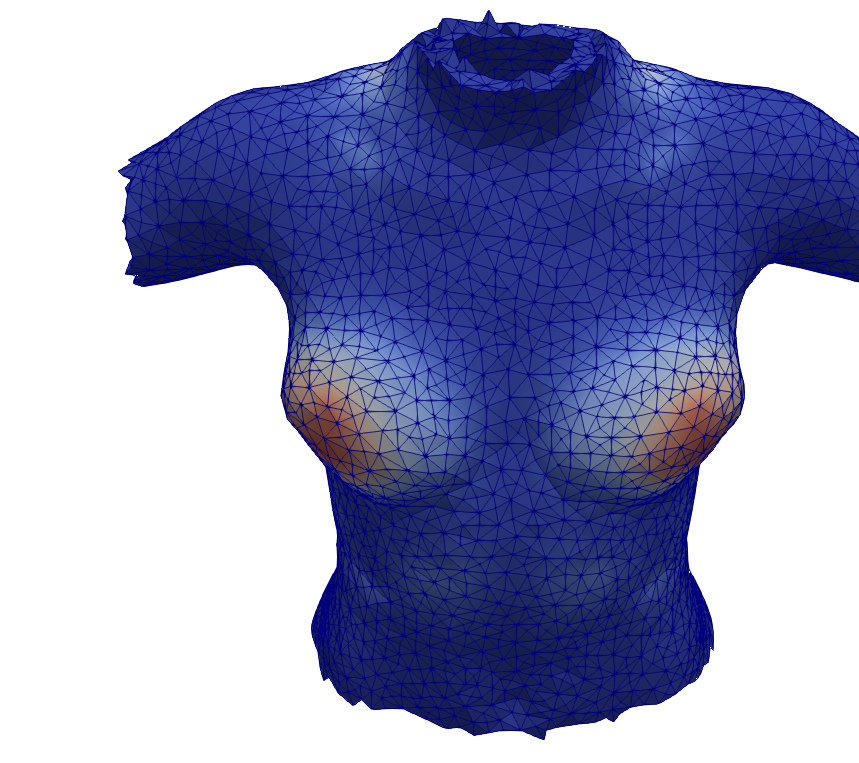
\includegraphics[width=1.0\textwidth]{images/cube_stretch/pr_045.png}}
		\caption*{(a) UNH, $\lambda = 10$}
		\label{sfig:stretch-snh10}
	\end{subfigure}\par\medskip
	\begin{subfigure}{1.0\linewidth}
		\centering
		\adjustbox{trim={.05\width} {.3\height} {.05\width} {.3\height},clip}%
		{\includegraphics[width=1.0\textwidth]{images/cube_stretch/pr_0495.png}}
		\caption*{(b) UNH, $\lambda = 100$}
		\label{sfig:stretch-snh100}
	\end{subfigure}\par\medskip
	\begin{subfigure}{1.0\linewidth}
		\centering
		\adjustbox{trim={.05\width} {.3\height} {.05\width} {.3\height},clip}%
		{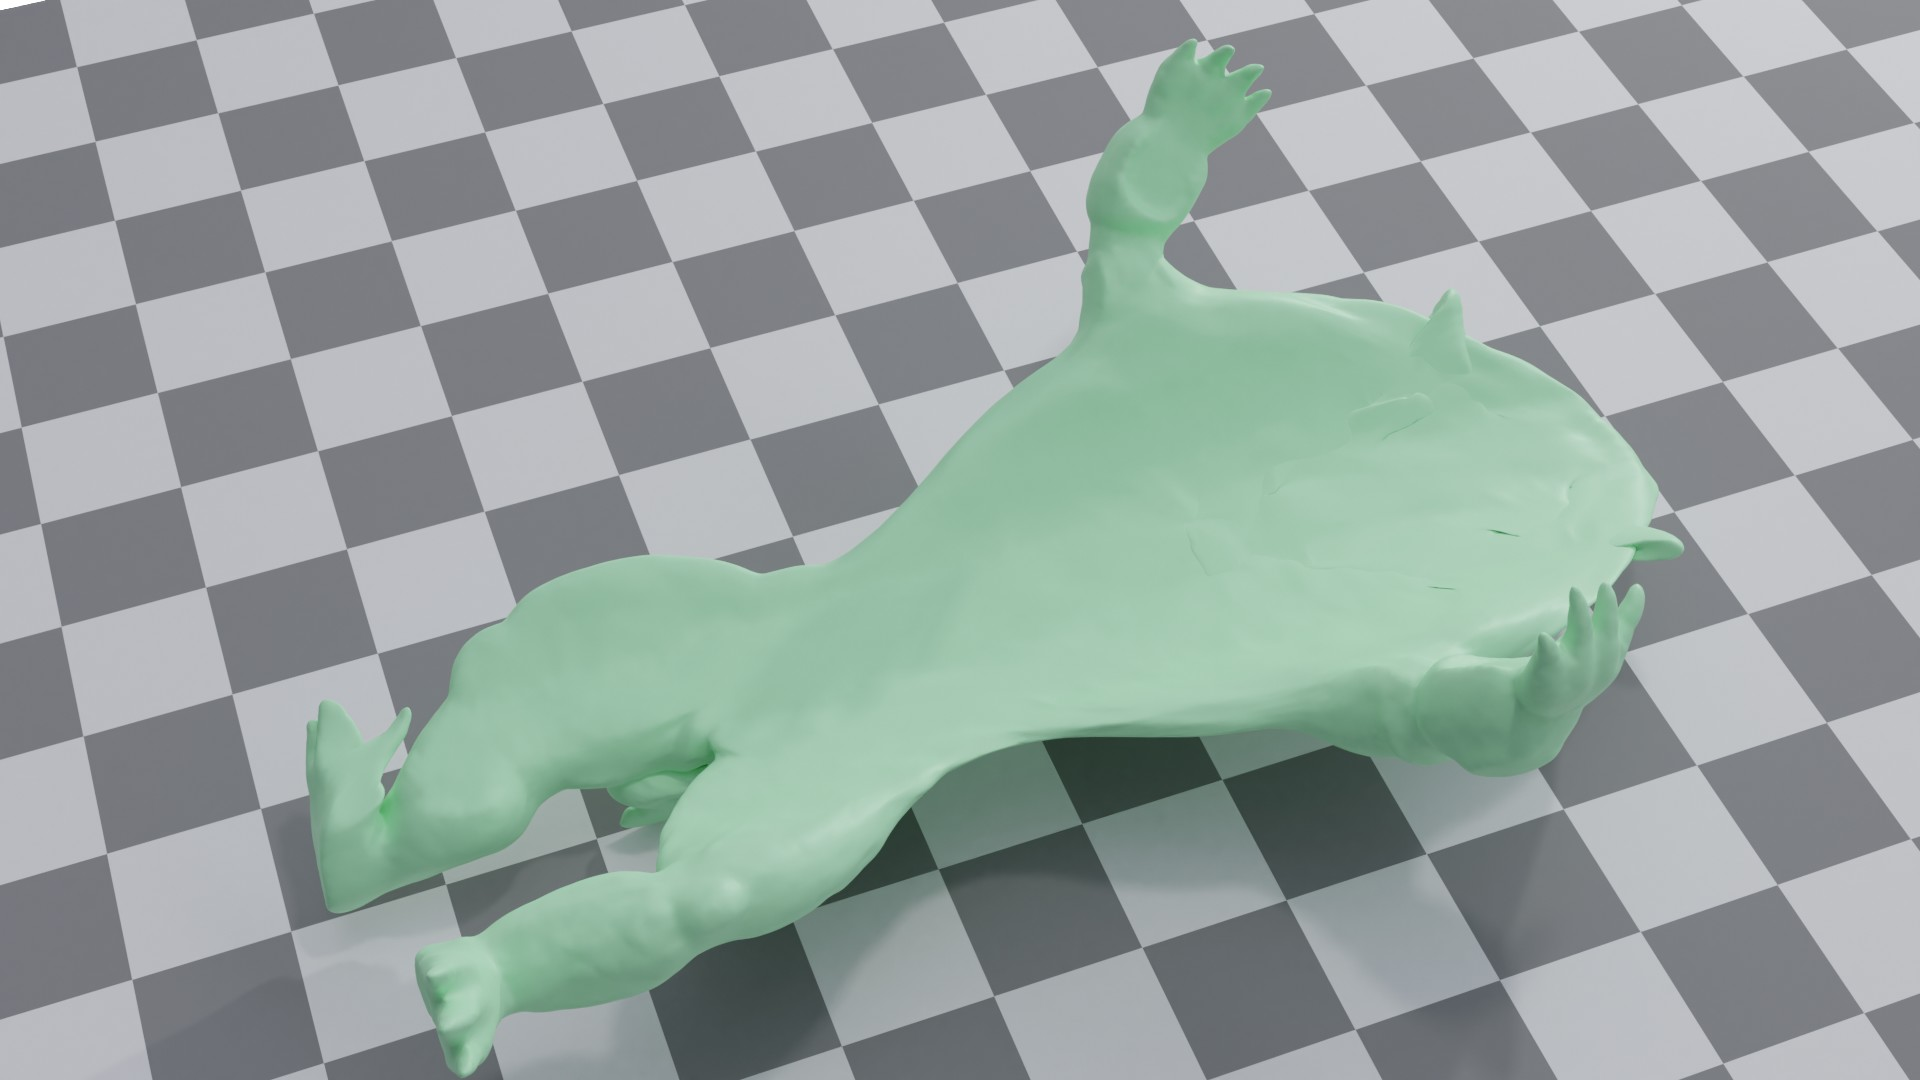
\includegraphics[width=1.0\textwidth]{images/cube_stretch/vc.png}}
		\caption*{(c) CNH, $\lambda = 25$}
		\label{sfig:stretch-vc}
	\end{subfigure}\par\medskip
	\begin{subfigure}{1.0\linewidth}
		\centering
		\adjustbox{trim={.05\width} {.3\height} {.05\width} {.3\height},clip}%
		{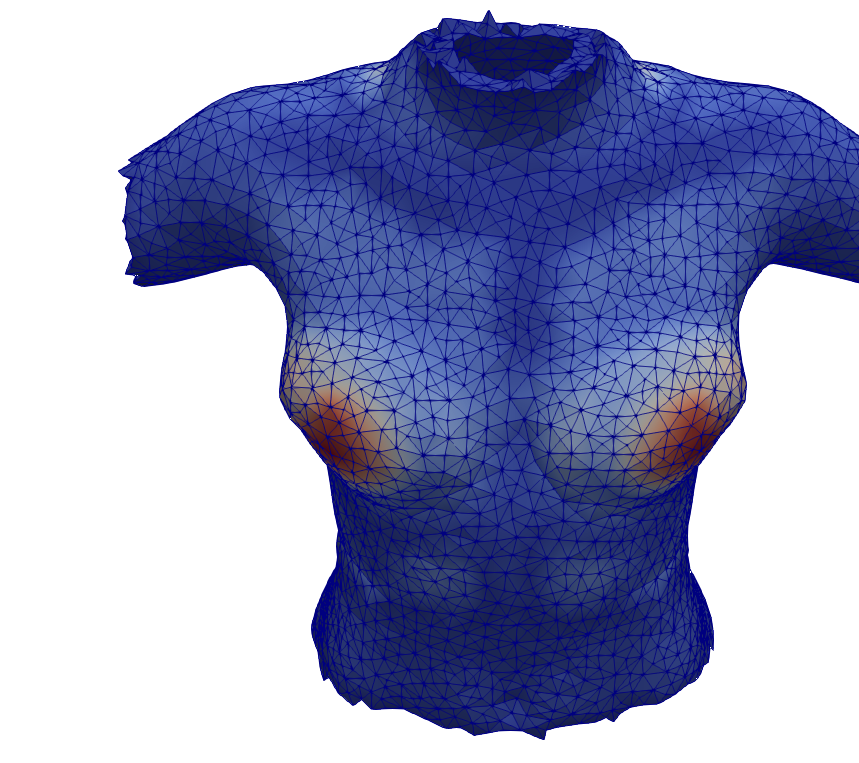
\includegraphics[width=1.0\textwidth]{images/cube_stretch/vc_epi.png}}
		\caption*{(d) CNH + Epidermis}
		\label{sfig:stretch-vcepi}
	\end{subfigure}%
	\caption{\textbf{Stretch}: A cube is stretched to eight times of its original length. (a) Using the unconstrained SNH with $\nu \approx 0.4545$, the volume error was ~14.83\% and tets became inverted around the cube corners (purple tets). (b) With $\nu = 0.495$, inverted tets were removed and the volume error is reduced to ~5.05\%. (c) When volume constraint ($\lambda = 25, \beta = 1$) is introduced, the volume is completely preserved and the simulation is 26.54\% faster. (d) With the epidermis ($\lambda_e = 10, \gamma = 1$) the deformed surface is regularized and the resulting deformation looks more organic. }
	\label{fig:cube-stretch}
\end{figure}


\section{Pressure Distribution}

\begin{figure}
	\centering
	\begin{subfigure}{.32\linewidth}
		\centering
		\adjustbox{trim={.15\width} {.00\height} {.15\width} {.00\height},clip}%
		{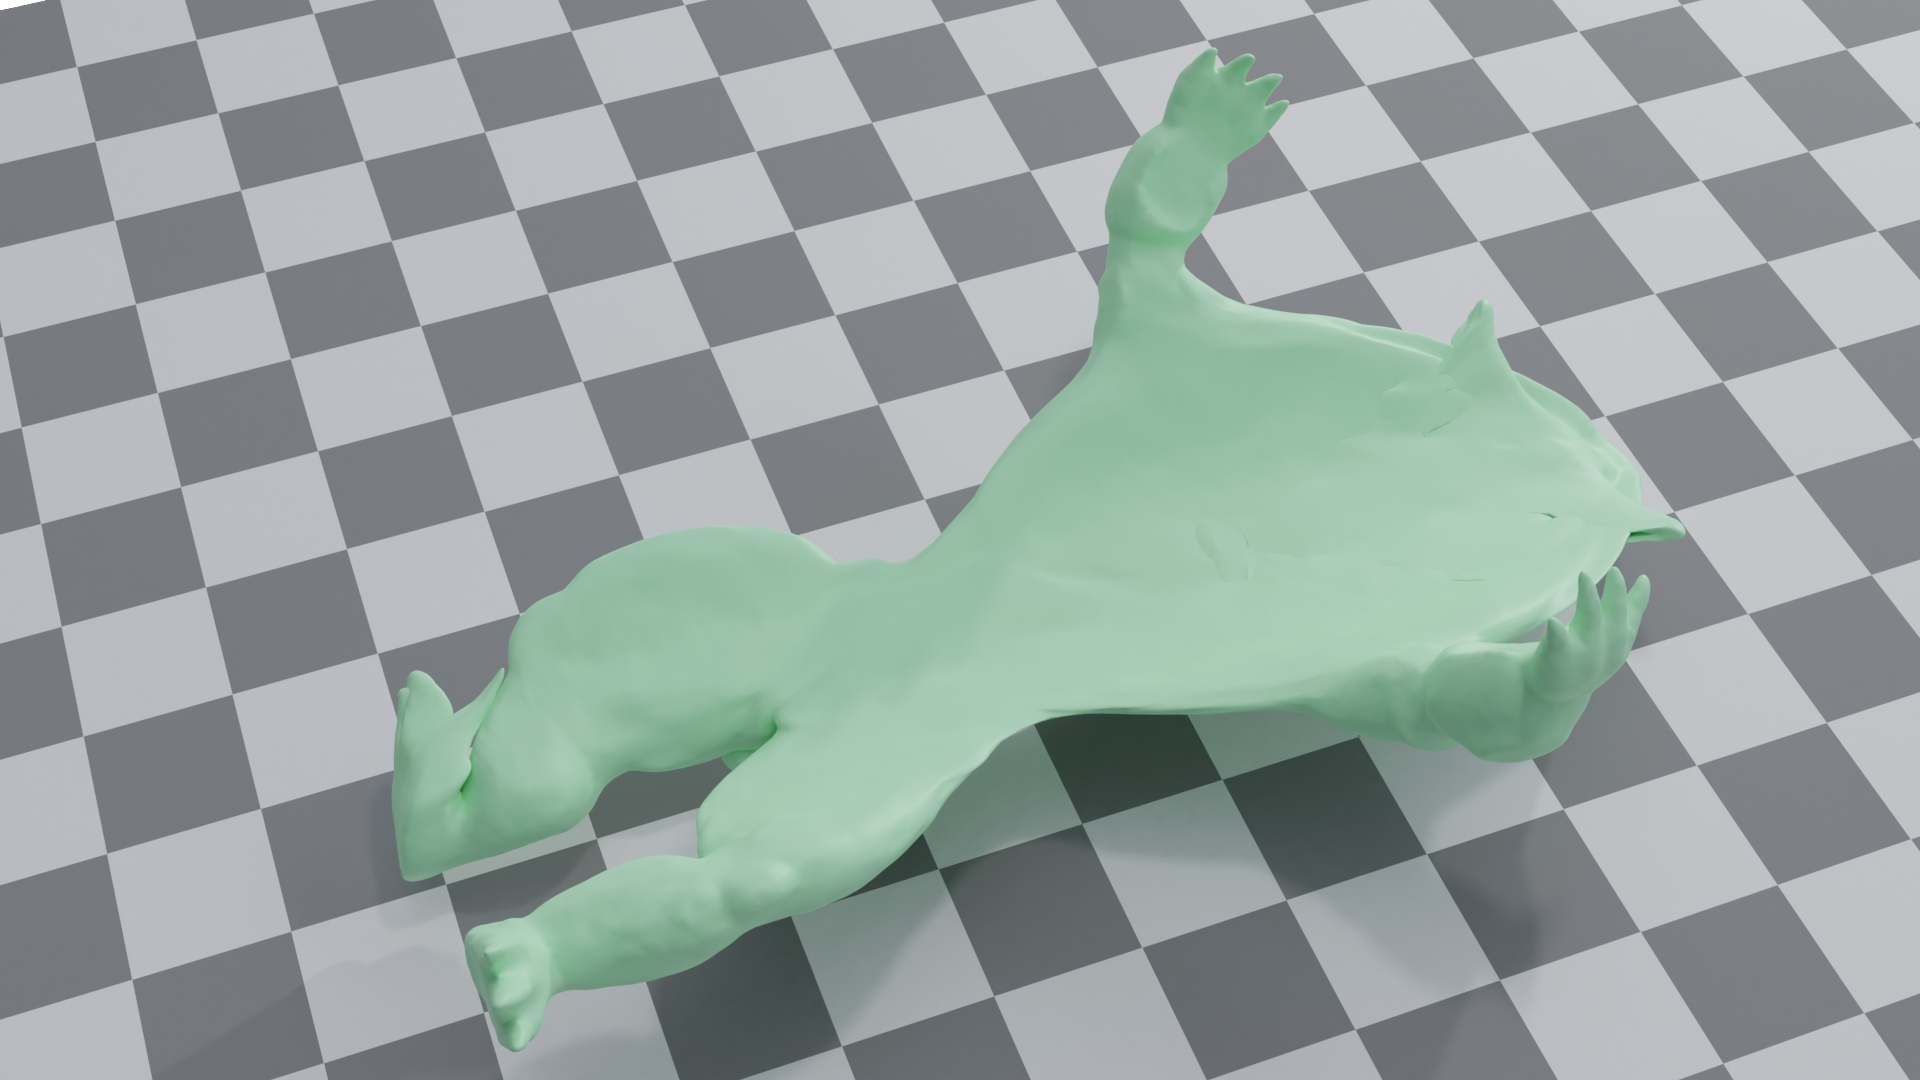
\includegraphics[width=1.3\textwidth]{images/suspended_cube/pr0495.png}}
		\caption*{(a) UNH, $\nu = 0.495$}
		\label{sfig:suspended-cube-pr-0495}
	\end{subfigure}%
	\begin{subfigure}{.32\linewidth}
		\centering
		\adjustbox{trim={.15\width} {.00\height} {.15\width} {.00\height},clip}%
		{\includegraphics[width=1.3\textwidth]{images/suspended_cube/onering.png}}
		\caption*{(b) One-ring}
		\label{sfig:suspended-cube-onering}
	\end{subfigure}%
	\begin{subfigure}{.32\linewidth}
		\centering
		\adjustbox{trim={.15\width} {.00\height} {.15\width} {.00\height},clip}%
		{\includegraphics[width=1.3\textwidth]{images/suspended_cube/vc100.png}}
		\caption*{(c) CNH, $\lambda = 100, \beta = 1$}
		\label{sfig:suspended-cube-vc-100}
	\end{subfigure}%
	\caption{\textbf{Pressure Distribution}: A cube with $12^3$ vertices is suspended under gravity with the bottom surface fixed with Dirichlet boundary conditions, visualized with the per-tet pressure distribution in the inner body. (a) shows the per-tet Poisson's ratio approach with $\nu = 0.495$, where the effects of volumetric locking results in highly irregular pressure distribution. (b) is the result where a one-ring volume constraint is used, where a checkerboard pattern appears in the pressure distribution due to a lack of stability. Finally, (c) is our method with $\lambda = 100, \beta = 1$, where the pressure distribution is regular and realistic. }
	\label{fig:suspended-cubes}
\end{figure}

Following a classic volumetric locking example, we test our methods with a standing cube simulation. A Neo-Hookean cube with shear modulus $\mu = 10.0$ is suspended under gravity with the bottom surface fixed with Dirichlet boundary conditions, results shown in Figure~\ref{fig:suspended-cubes}. This example demonstrates the effects of external force on the pressure distribution on the body surface and interior with regards to different approaches of simulating incompressibility. Irregular pressure distribution may not visually affect the results much, but when simulating frictional contact or fracture, they might result in unrealistic solutions. The high Poisson's ratio ($\nu = 0.495$) approach results in obvious irregularities in the pressure distribution, a manifestation of volumetric locking. The per-tet hydrostatic pressures in this case are computed as the the volumetric components of the stress tensors, that is, the negative divergence of the Cauchy stress. The high bulk modulus per each element causes pressure computation from displacement variables to be unreliable. The one-ring volume constraint approach \cite{Irving:2007}, which is equivalent to the Average Nodal Pressure element \cite{bonet:1998}, shows a more regular pressure distribution, but also shows checkerboard patterns. In this case, the pressures are the Lagrange multipliers for the volume constraints, scaled to be in the same units as the volumetric stress then mapped back to the cells. The checkerboard pattern is an artifact of the instability of the one-ring constraint approach, where the averaging of the pressure variables on the nodes allows solutions with such checkerboarding to occur. With our method with one global zone and a local compression penalty of $\lambda = 100, \beta = 1$, we compute the per-tet pressure as a sum of the average zonal pressure (the Lagrange multiplier of the zonal volume constraint) and the fine-scale pressures computed from the volumetric stress component from the penalty. Then since the bulk modulus is much smaller, as opposed to $(\nu = 0.495) \equiv (\lambda = 400)$ in the Poisson's ratio approach, volumetric locking does not happen from the penalty, and therefore the volumetric stress components are more regular. Since the volume preserving zone is global and since the average pressure is constant throughout the zone, checkerboard pattern in the Lagrange multipliers is not an issue. 

\section{Dynamic Stability}

\begin{figure}
	\centering   	
	\begin{overpic}[width=1.0\columnwidth]{images/energy_plot.pdf}
		\put(30,30){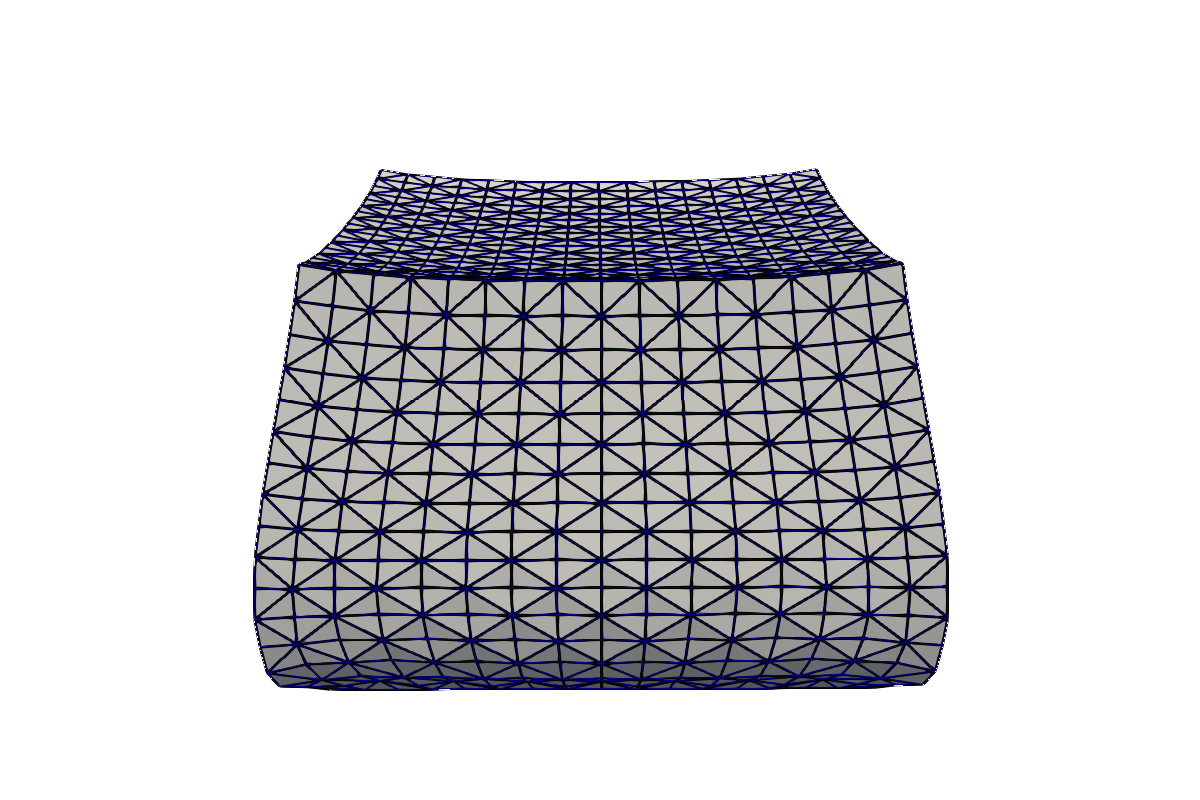
\includegraphics[width=0.3\columnwidth]{images/rep.png}}  
		\put(49.5,14){
			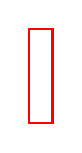
\begin{tikzpicture}
				\draw[thick,draw=red] (0,0) rectangle ++(0.3,1.2);
			\end{tikzpicture}	
		}
		\put(58,14){
			
\begin{tikzpicture}
				\draw[thick,draw=yellow] (0,0) rectangle ++(2.1,1.2);
			\end{tikzpicture}	
		}
	\end{overpic} \hfill
	\begin{overpic}[width=0.45\columnwidth]{images/energy_plot_zoom.pdf}
		\put(0,-0.2){
			\begin{tikzpicture}
				\draw[thick,draw=red] (0,0) rectangle ++(5.4,2.9);
			\end{tikzpicture}	
		}
	\end{overpic} \hfill
	\begin{overpic}[width=0.45\columnwidth]{images/energy_plot_zoom2.pdf}
		\put(0,-0.2){
			\begin{tikzpicture}
				\draw[thick,draw=yellow] (0,0) rectangle ++(5.4,2.9);
			\end{tikzpicture}	
		}
	\end{overpic}
	\caption{\textbf{Dynamic Stability}: Energy plot from the simulation of a soft $16^3$ cell cube subjected to gravity, with a moderately large timestep of 8ms. We compare three different algorithms for simulating incompressibility, where the blue curve is the energy plot for the one-ring pressure algorithm of \cite{Irving:2007}, the red is a na\"ive global volume rescaling algorithm, and yellow is ours. \cite{Irving:2007} (blue) shows severe instability even with an aggressive clamping of the volume recovery. Note how due to the extreme oscillations in potential energy, the energy plot for the method appears as a thick line in the top plot. The bottom plots show a magnified plot to demonstrate how the energy behaves in small timeframes. The volume rescaling algorithm (green) gains and loses energy arbitrarily due to a unrealistic simulation of the volumetric stress, which can be seen from the irregularities in the plot. Our method (yellow) displays a realistic and stable energy behavior, and converges to a stable configuration. \label{fig:stability}}
\end{figure}


We test the stability of our method in dyanamic simulations compared to \cite{Irving:2007} and a na\"ive volume rescaling method. We simulate a cube consisting of $16^3$ cells with $\mu = 100.0$ is subjected under gravity. We tested the simulation with a timestep of 8ms for a total of 1000 frames.
We found that the volume projection in the Irving algorithm can be unstable when used with large timesteps, and a clamping of volume preservation forces must be applied to make it stable. However, we found that the clamping threshold to make this specific example not blow up was quite low, resulting in a volume error of ~2.4\% at worst. Even with such aggressive clamping, we noticed visible oscillations on the top surface of the cube.
We also tested a simple volume rescaling algorithm, where the mesh was projected every time step based on its center of mass, such that the global volume is conserved. We found that this method is highly unstable and virtually impossible with Semi-Implicit Euler integration (where only one Newton step is used) without increasing Poisson Ratio to higher than 0.495, where then locking occurs instead. With full Backwards Euler integration, we could get the simulation to not blow up, but it still required a quite high Poisson Ratio of 0.48. However, a unrealistically exaggerated oscillation of the entire mesh was present even until the final frames. 
Compared to the other methods, we found our method to be very stable, and the runtimes were comparable (around 2\% faster) to Irving's, which is a semi-implicit method where ours is fully implicit. With our method, this simulation is stable at much higher timesteps, i.e. 33ms. 


The plot of the potential energy for this simulation can be seen Figure~\ref{fig:stability}. Note the extreme oscillations present in the potential energy plot for the one-ring nodal pressure algorithm \cite{Irving:2007} and the unrealistic irregularities in the plot for the volume rescaling algorithm.


\section{Bulge Test}

\begin{figure}
	\centering
	\begin{subfigure}{.24\linewidth}
		\centering
		\includegraphics[width=1.0\textwidth]{images/puck/pr0495_25.png}
		\includegraphics[width=1.0\textwidth]{images/puck/pr0495_50.png}
		\adjustbox{trim={.15\width} {.0\height} {.15\width} {.1\height},clip}%
		{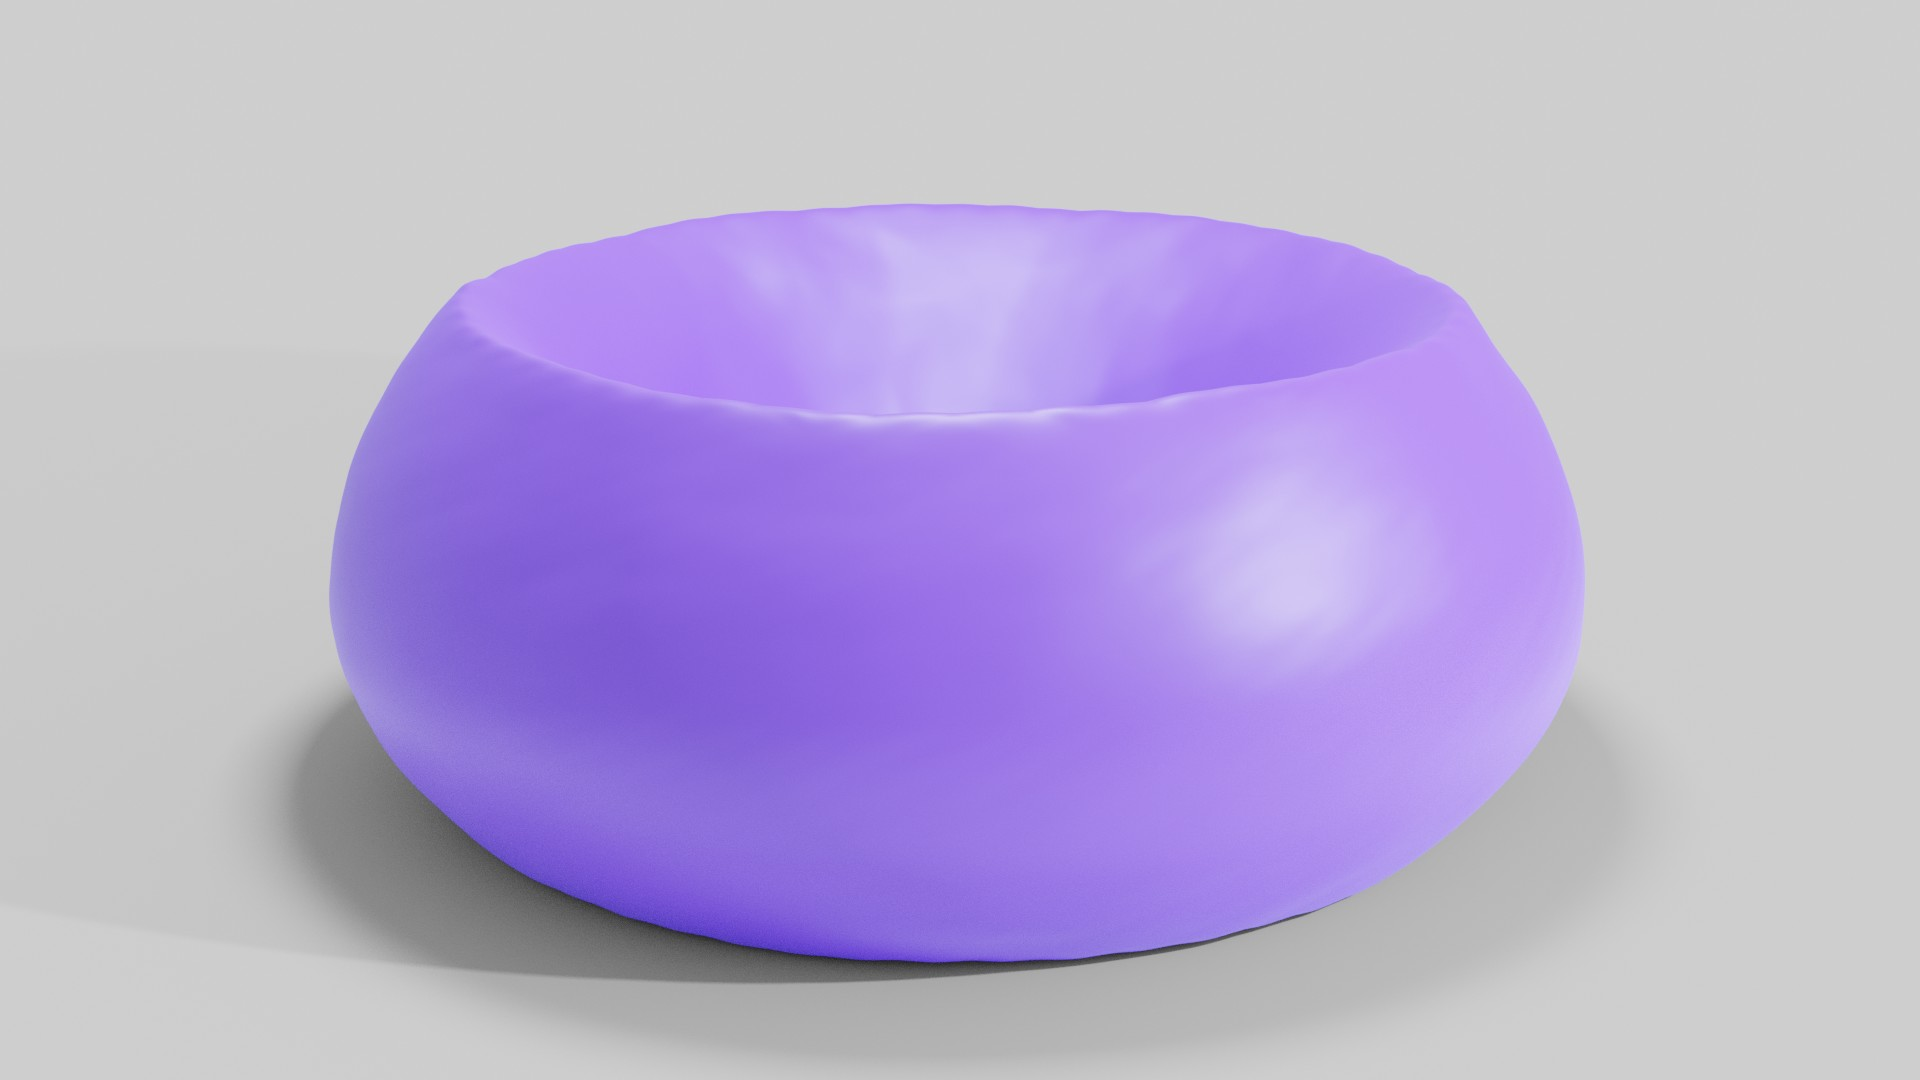
\includegraphics[width=1.4\textwidth]{images/puck/pr0495_render.jpg}}
		\caption*{(a) UNH, $\nu = 0.495$}
		\label{sfig:puck-pr0495}
	\end{subfigure}%
	\begin{subfigure}{.24\linewidth}
		\centering
		\includegraphics[width=1.0\textwidth]{images/puck/pr04545_25.png}
		\includegraphics[width=1.0\textwidth]{images/puck/pr04545_50.png}
		\adjustbox{trim={.15\width} {.0\height} {.15\width} {.1\height},clip}%
		{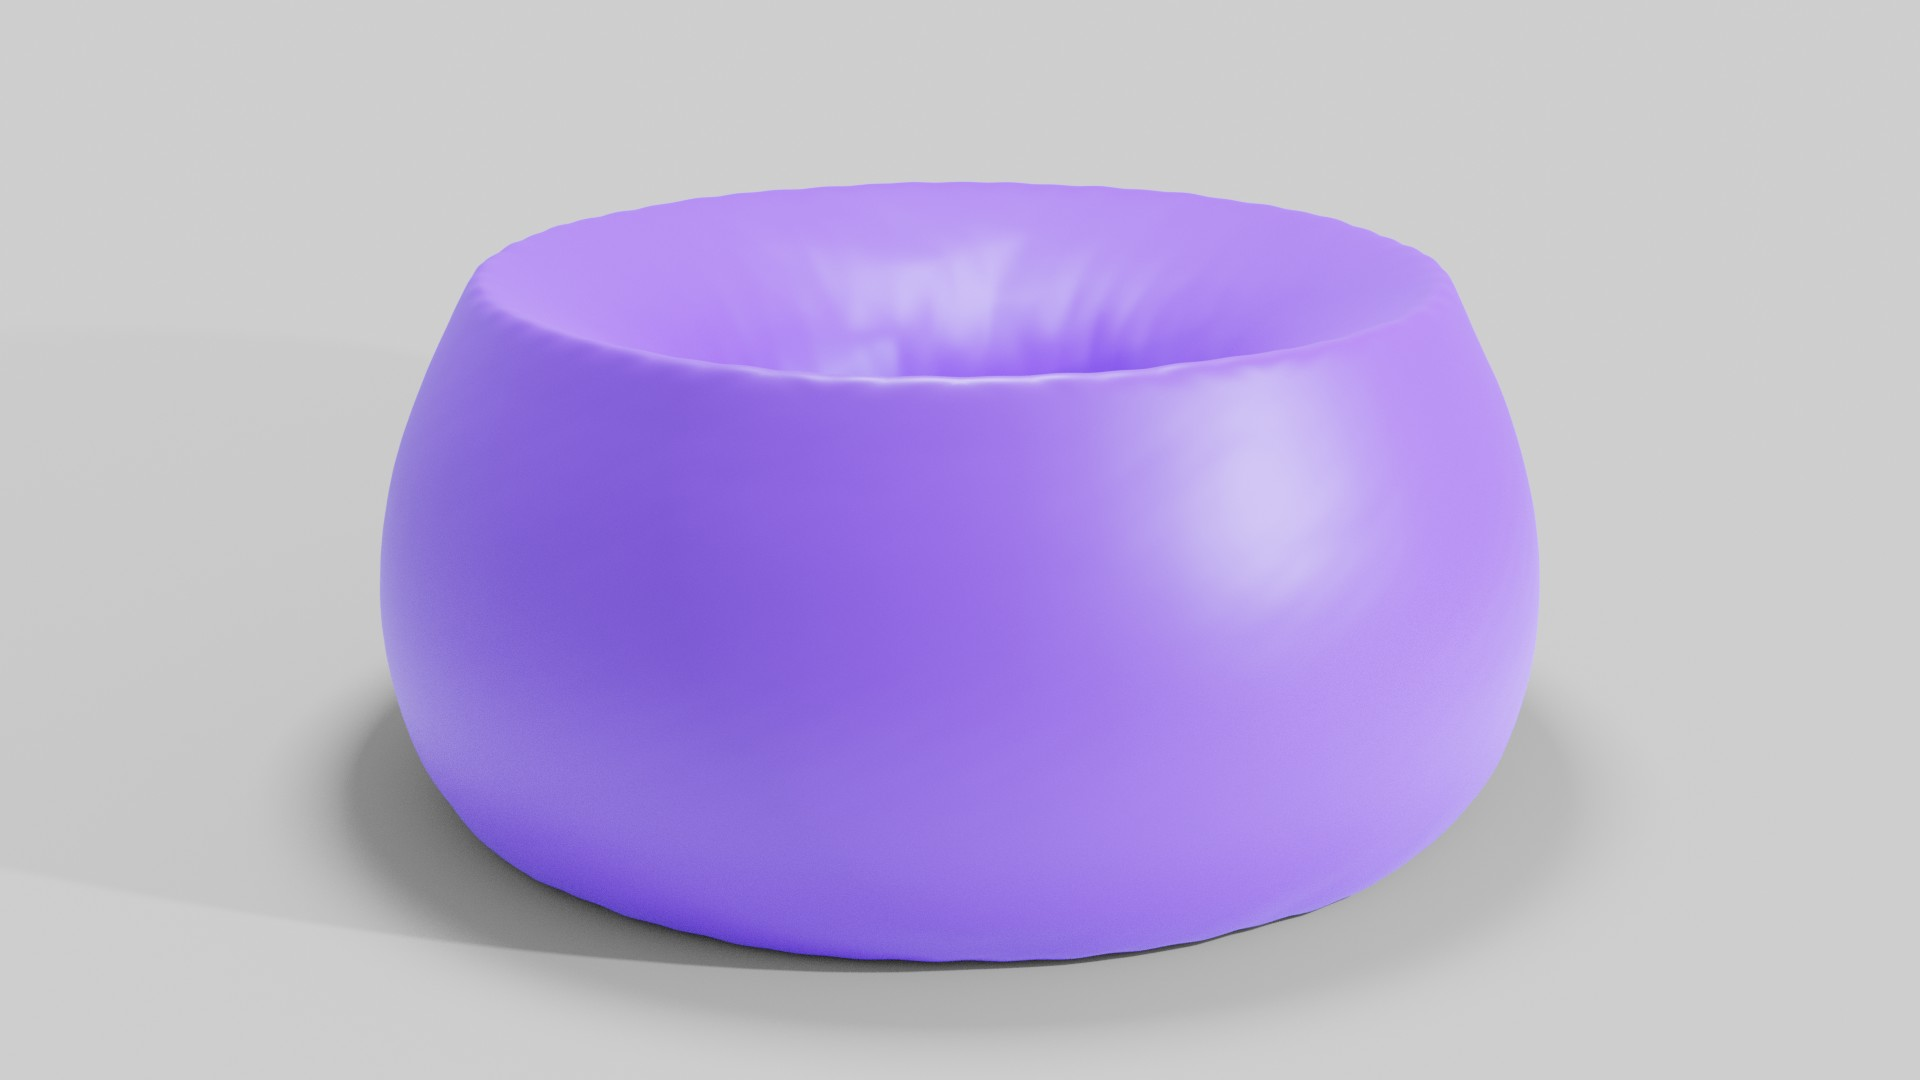
\includegraphics[width=1.4\textwidth]{images/puck/pr045_render.jpg}}
		\caption*{(b) UNH, $\nu = 0.4545$}
		\label{sfig:puck-pr04545}
	\end{subfigure}%
	\begin{subfigure}{.24\linewidth}
		\centering
		\includegraphics[width=1.0\textwidth]{images/puck/vc60-15_25.png}
		\includegraphics[width=1.0\textwidth]{images/puck/vc60-15_50.png}
		\adjustbox{trim={.15\width} {.0\height} {.15\width} {.1\height},clip}%
		{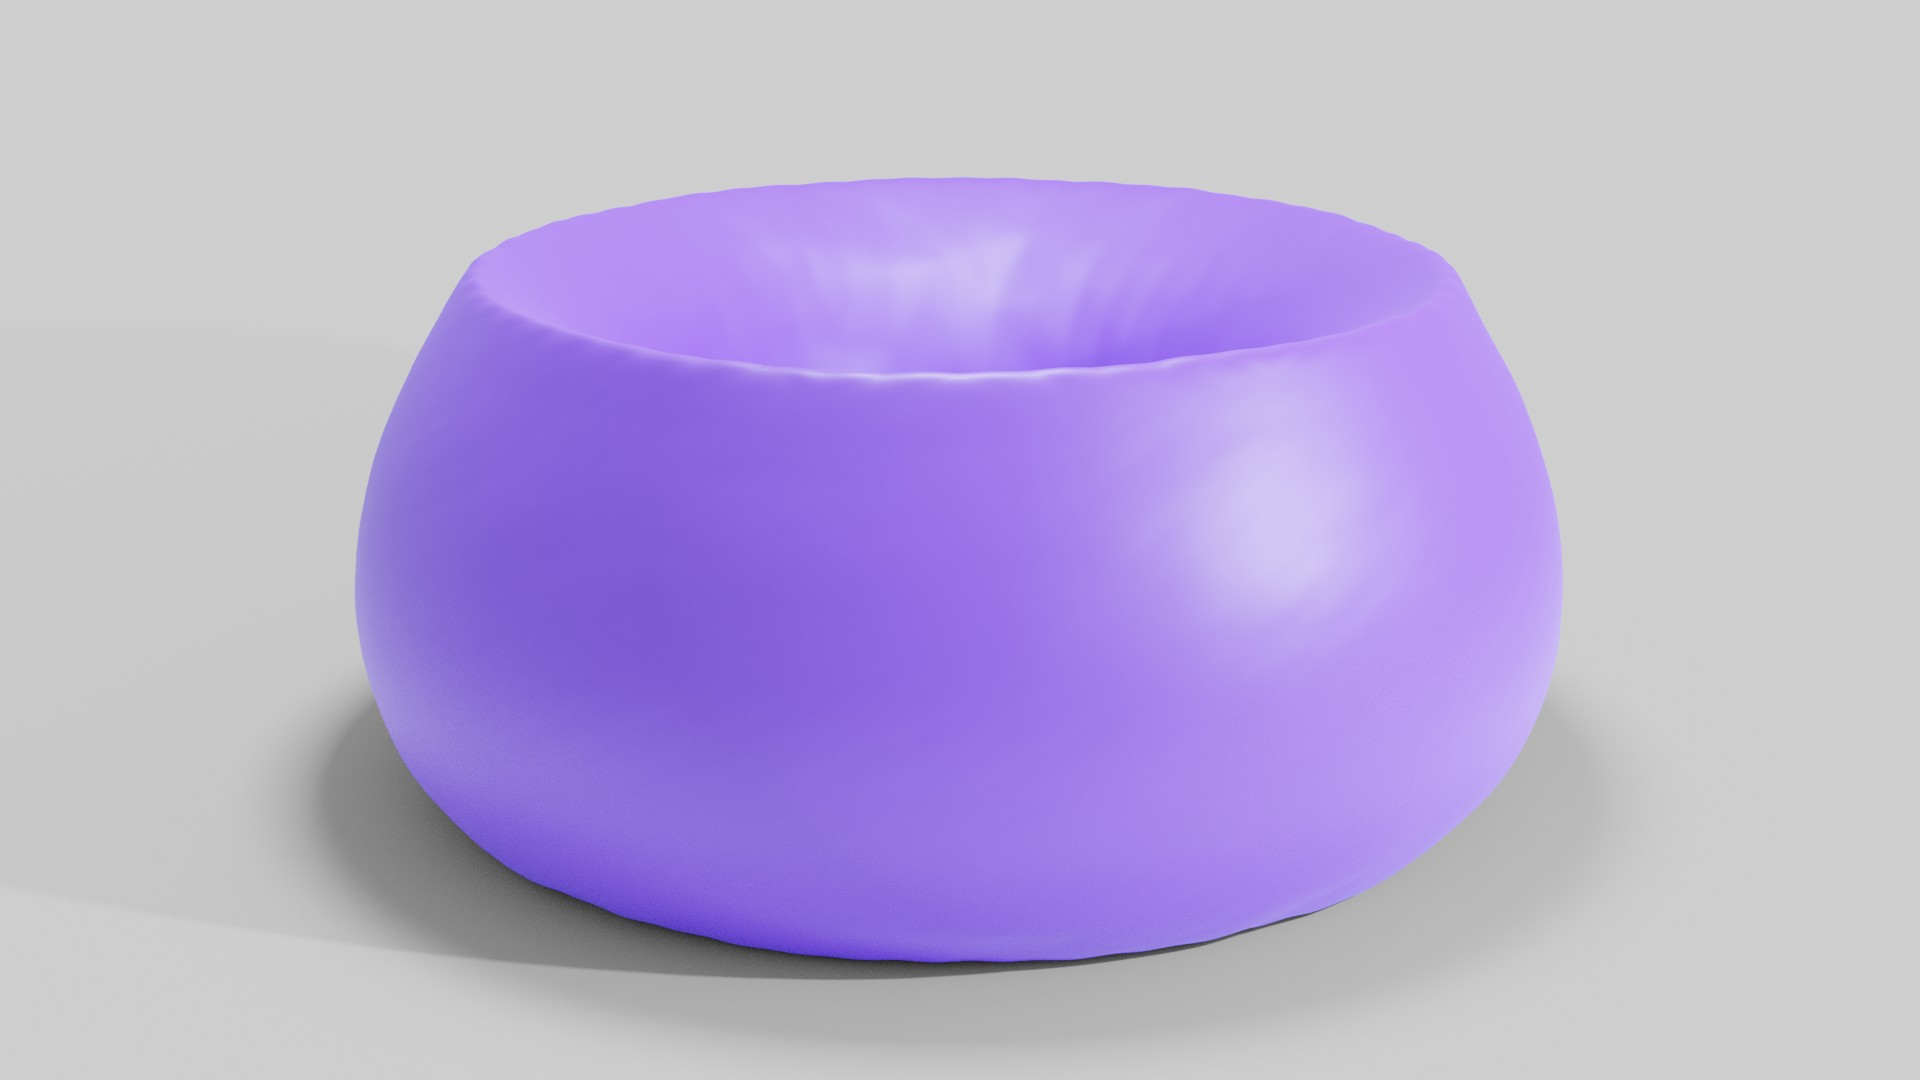
\includegraphics[width=1.4\textwidth]{images/puck/vc_render.jpg}}
		\caption*{(c) CNH}
		\label{sfig:puck-vc}
	\end{subfigure}%
	\begin{subfigure}{.24\linewidth}
		\centering
		\includegraphics[width=1.0\textwidth]{images/puck/vc60-15_epi40_25.png}
		\includegraphics[width=1.0\textwidth]{images/puck/vc60-15_epi40_50.png}
		\adjustbox{trim={.15\width} {.0\height} {.15\width} {.1\height},clip}%
		{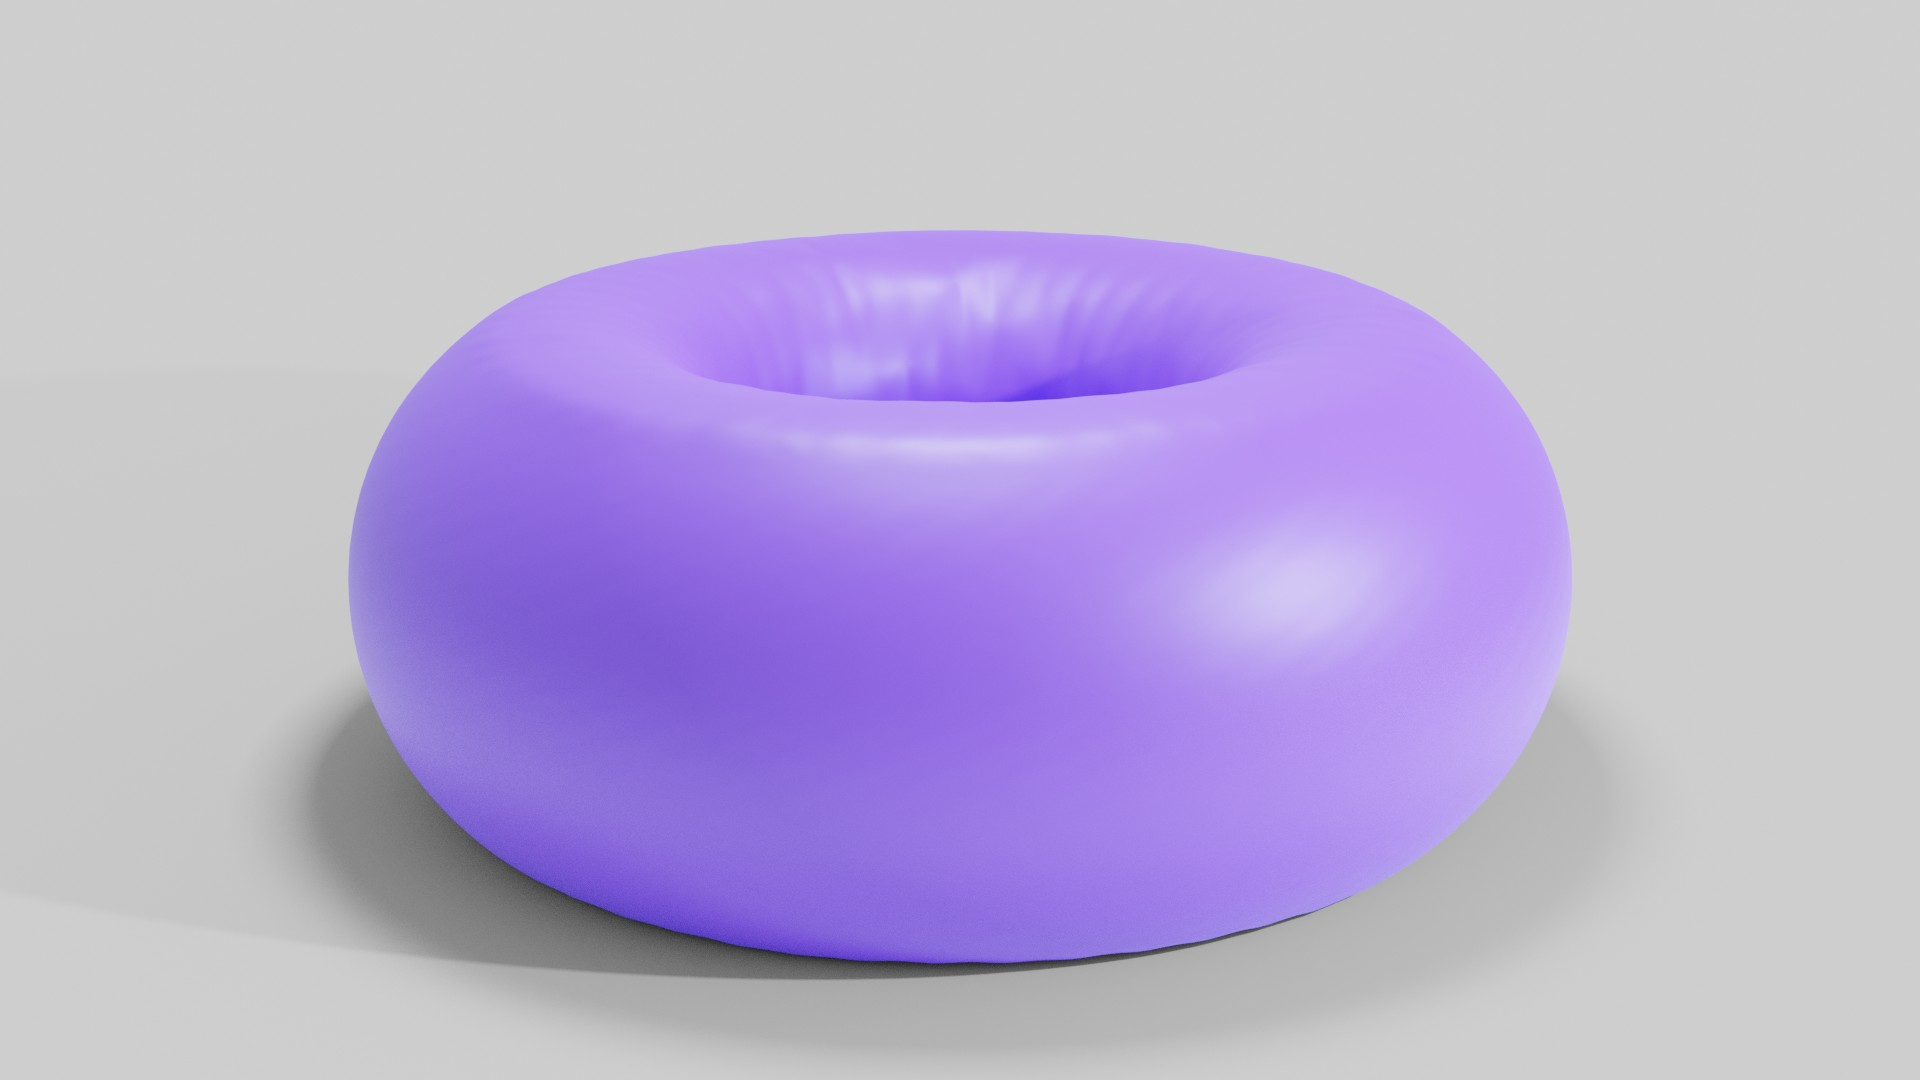
\includegraphics[width=1.4\textwidth]{images/puck/vc_epi_render.jpg}}
		\caption*{(d) CNH + Epidermis}
		\label{sfig:puck-vc-epi}
	\end{subfigure}%
	\caption{\textbf{Bulge Test}: A cross-section of a simulated puck is shown. The puck is indented at $25\%$ and $50\%$ of its height. (a) is the result without volume constraint and $\nu = 0.495$. These base results show visible volume loss of $0.6\%$ and $1.8\%$ and artificial stiffness from locking, resulting in no visible bulging at the cylinder top. Also, the pressure distribution visualized by the color scheme shows severe irregularities. (b) is the simulation with $\nu = 0.4545$, which loses $2.1\%$ and $5.1\%$ of the total volume respectively. (c) shows the result with volume constraint and $\lambda = 100$ and $\beta = 9$, showing a realistic bulging due to successful volume preservation. (d) shows the result where an epidermis of $\lambda = 100$ was added, where the surface demonstrates a more organic deformation due to surface volume preservation. }
	\label{fig:pucks}
\end{figure} 

One good natural example of an incompressible material is the human tissue, so to test the effects of our method, we test on the ``skin puck'' model from \cite{Pai:2018}, where the vertices on the bottom are fixed with Dirichlet boundary conditions. 
When simulating biological tissue, bulging is a crucial visual characteristic that depicts the incompressibility of the underlying material. 
Therefore, it is important that this simulation shows visually significant bulging under compression.

We use a 22K tetrahedron simulation mesh for the puck.  To produce substantial compression, we animate a set of vertices on the top of the puck with a Dirichlet boundary condition moving these vertices down by a fixed amount per time step. We performed a quasi-static simulation where at each step, the animated surface is indented by 1\% of the height. We test the displacement until 50\% of the total height of the puck, which produces extreme compression.

Without the volume constraint, a low Poisson's Ratio $\nu \in [0.0, 0.45]$ will result in little noticeable bulging at the top surface due to volume loss, and a higher $\nu$ will result in unnaturally stiff visual results and irregular pressure distribution due to volumetric locking. Also, even at $\nu = 0.495$, there was a $1.8\%$ volume loss at an indentation of 50\% of the puck height.

Adding the volume constraint allows a completely incompressible simulation with realistic pressure solutions for this example, without being a heavy burden on the performance in most cases. At $50\%$ indentation, the amount of volume loss can be made arbitrarily low\footnote{Up to machine precision.} with the global volume constraint using any type of energy model and parameters. In contrast, a standard simulation without the constraint produces approximately 22\% volume loss with $\nu = 0.4$, 5.1\% loss with $\nu = 0.45$, and 1.8\% loss with $\nu = 0.495$. However, without any local compression penalty the simulation converges to an infeasible state with many inverted tets around the border of the Dirichet boundaries.

Adding our local penalty term with $\lambda = 100$ allows the simulation to be completely free of inverted tets. Although even with $\beta = 0$ the solution does not converge to an infeasible state, the lack of a sufficient resistance to volumetric deformation causes numerical instability and results in a very slow convergence of the nonlinear optimizer during the timesteps with more extreme deformations (after the 25\% indentation). By using $\beta = 9$ we were able to achieve better numerical stability, resulting in a 14.84\% faster runtime on total, and 21.17\% faster runtime when only considering the frames after the 25\% indentation where the moving Dirichlet boundary starts to invert elements. Finally, with an epidermis model of $\lambda_e = 100, \beta_e = 1$ added, we are able to generate a more regular surface deformation and achieve an visually organic deformation overall. 

\section{Dynamic Impact}

\begin{figure}
	\centering
	\begin{subfigure}{.03\linewidth}
		\rotatebox[origin=c]{90}{\footnotesize{\quad(a) UNH, $\nu=0.45$}}
	\end{subfigure}%
	\begin{subfigure}{.16\linewidth}
		\centering
		\adjustbox{trim={.25\width} {.0\height} {.25\width} {.4\height},clip}%
		{\includegraphics[width=2.0\textwidth]{images/soft_ball/045/0200.jpg}}
		%\caption*{(a1)}
		\label{sfig:ball-045-1}
	\end{subfigure}%
	\begin{subfigure}{.16\linewidth}
		\centering
		\adjustbox{trim={.25\width} {.0\height} {.25\width} {.4\height},clip}%
		{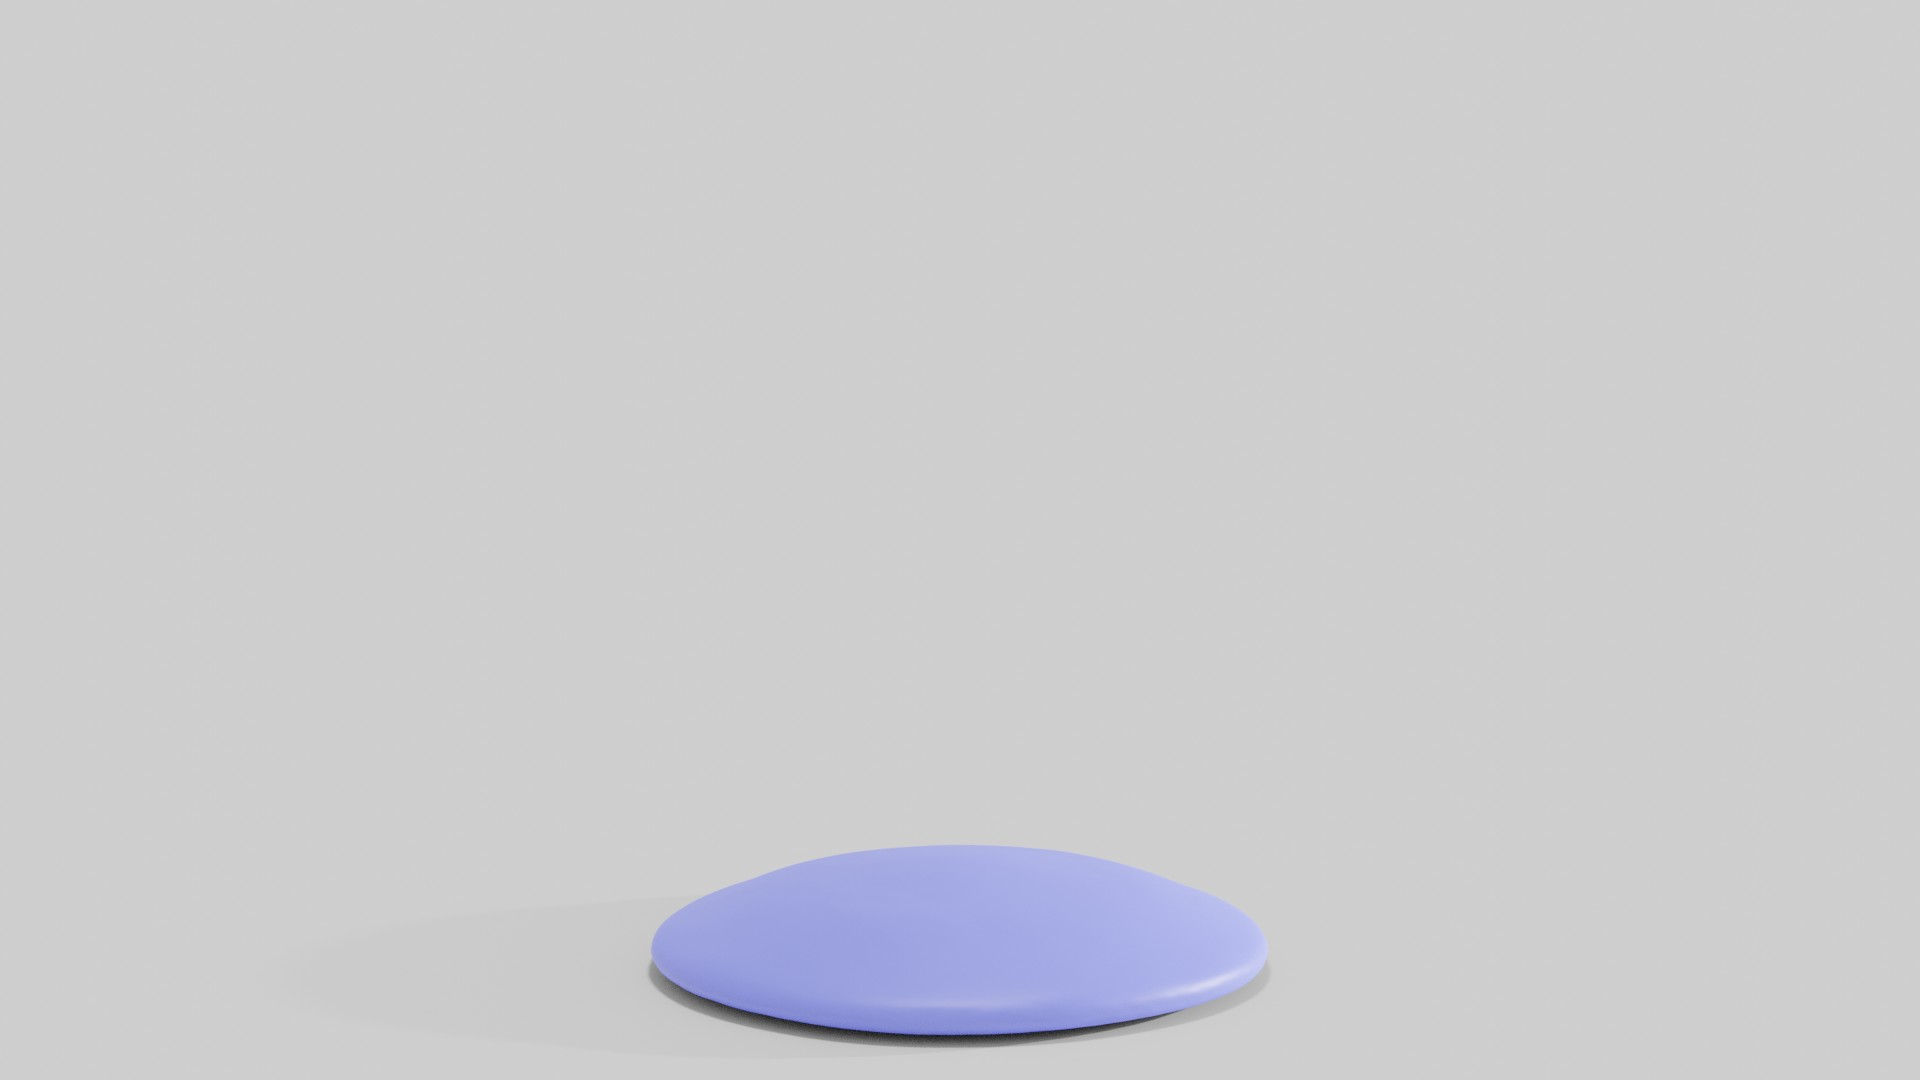
\includegraphics[width=2.0\textwidth]{images/soft_ball/045/0250.jpg}}
		%\caption*{(a2)}
		\label{sfig:ball-045-2}
	\end{subfigure}%
	\begin{subfigure}{.16\linewidth}
		\centering
		\adjustbox{trim={.25\width} {.0\height} {.25\width} {.4\height},clip}%
		{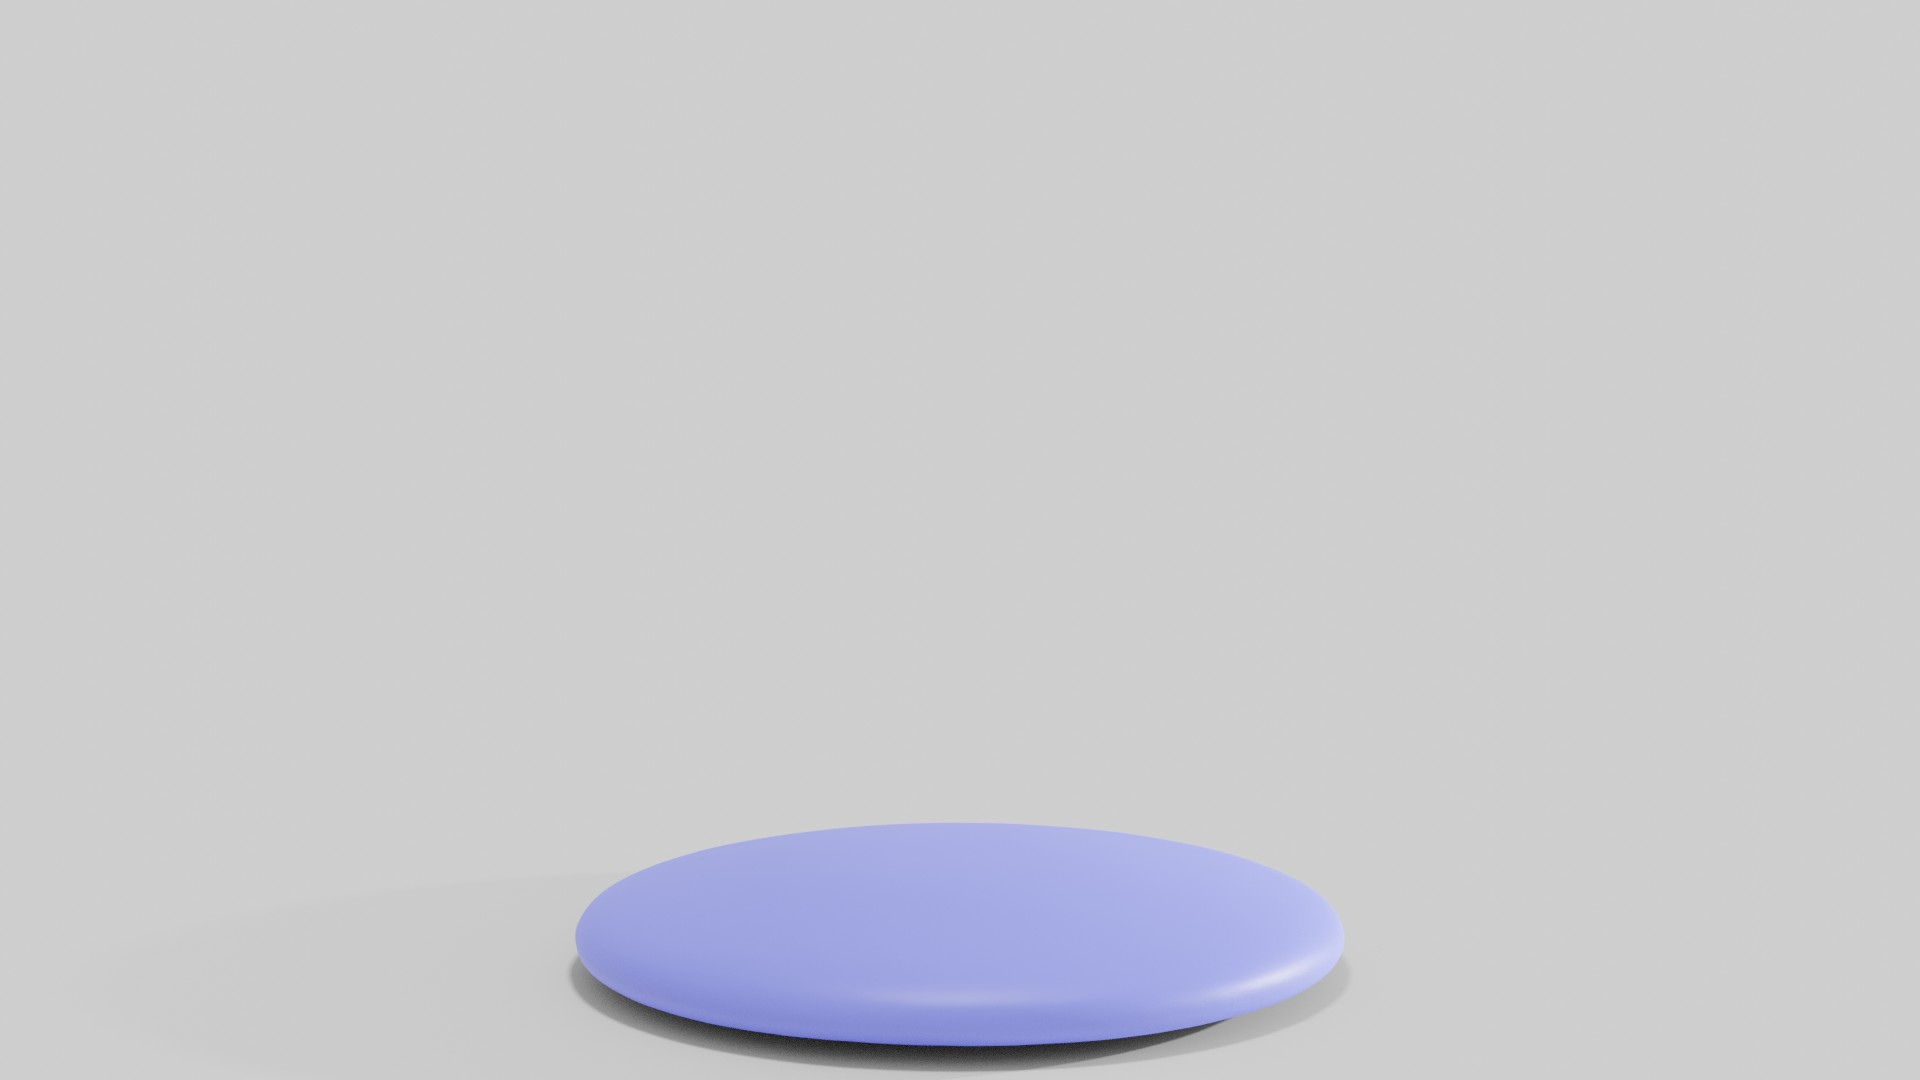
\includegraphics[width=2.0\textwidth]{images/soft_ball/045/0300.jpg}}
		%\caption*{(a3)}
		\label{sfig:ball-045-3}
	\end{subfigure}%
	\begin{subfigure}{.16\linewidth}
		\centering
		\adjustbox{trim={.25\width} {.0\height} {.25\width} {.4\height},clip}%
		{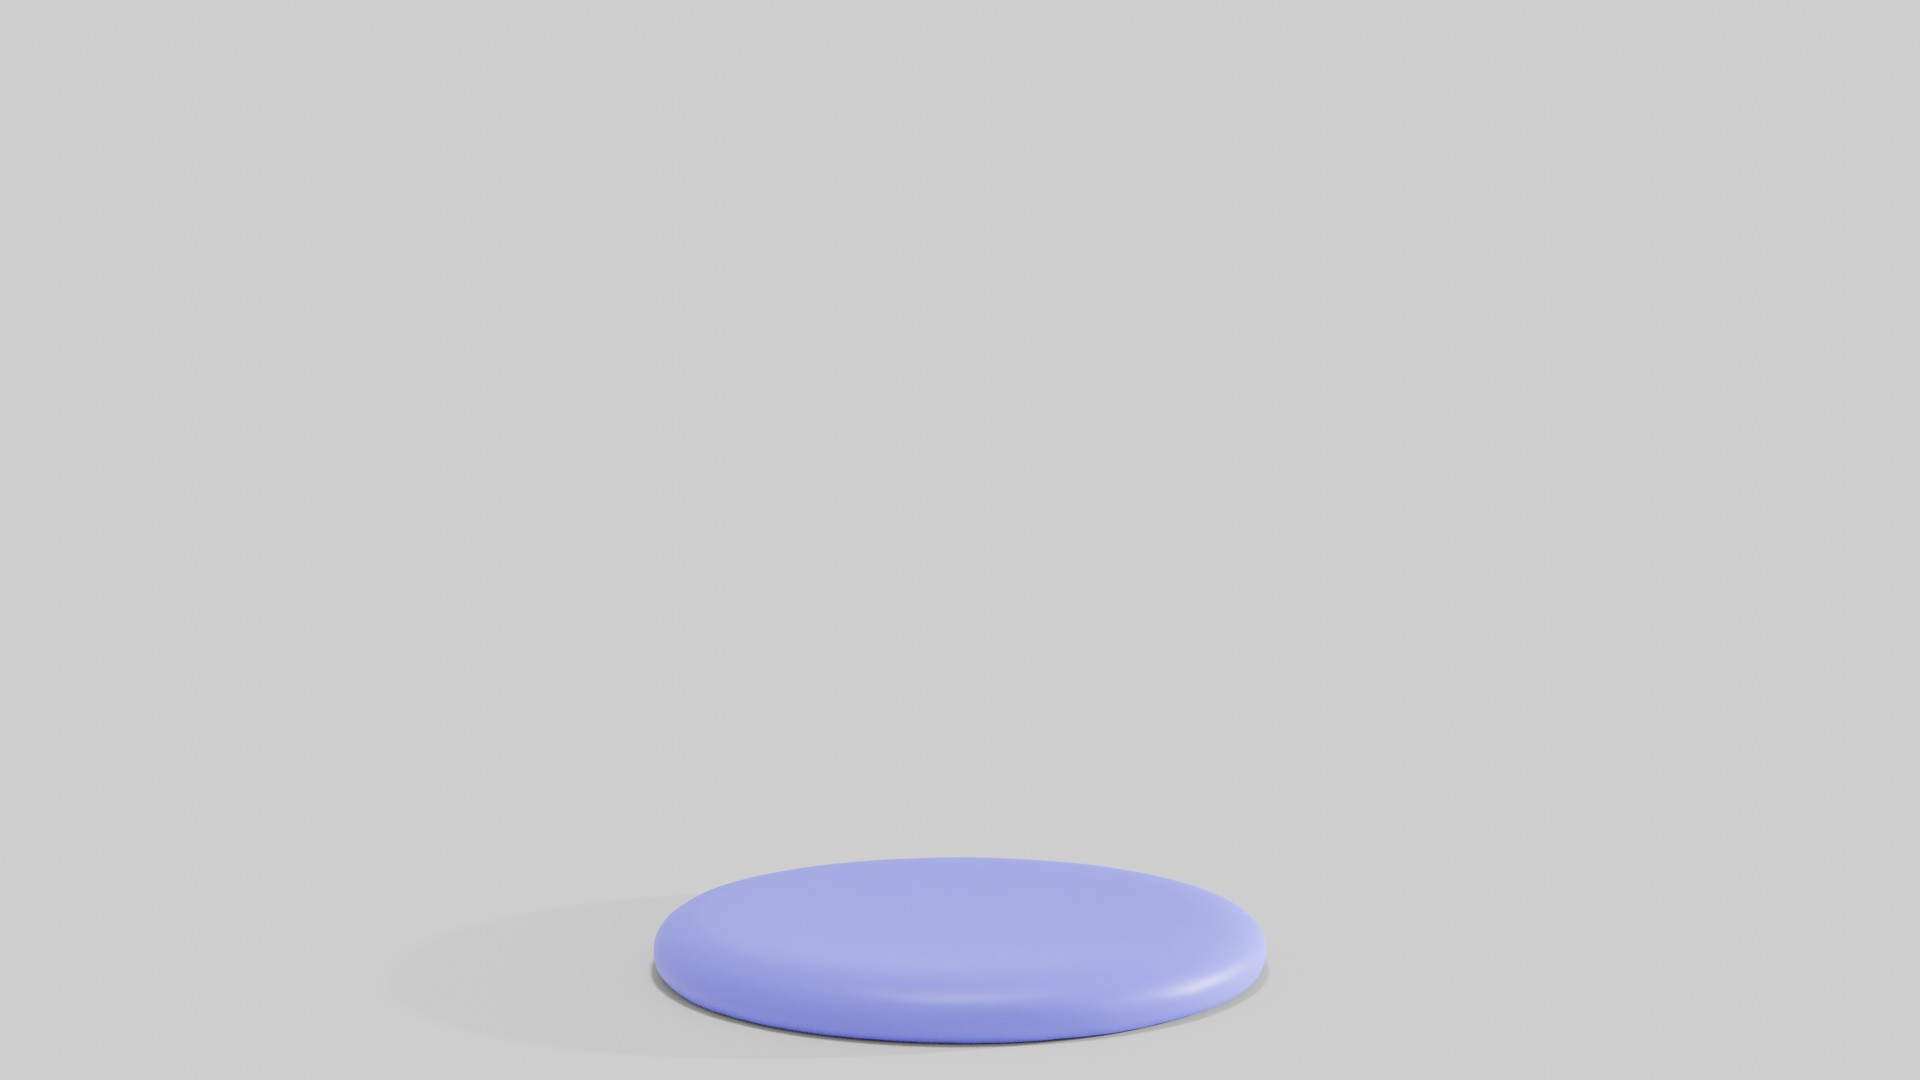
\includegraphics[width=2.0\textwidth]{images/soft_ball/045/0350.jpg}}
		%\caption*{(a4)}
		\label{sfig:ball-045-4}
	\end{subfigure}%
	\begin{subfigure}{.16\linewidth}
		\centering
		\adjustbox{trim={.25\width} {.0\height} {.25\width} {.4\height},clip}%
		{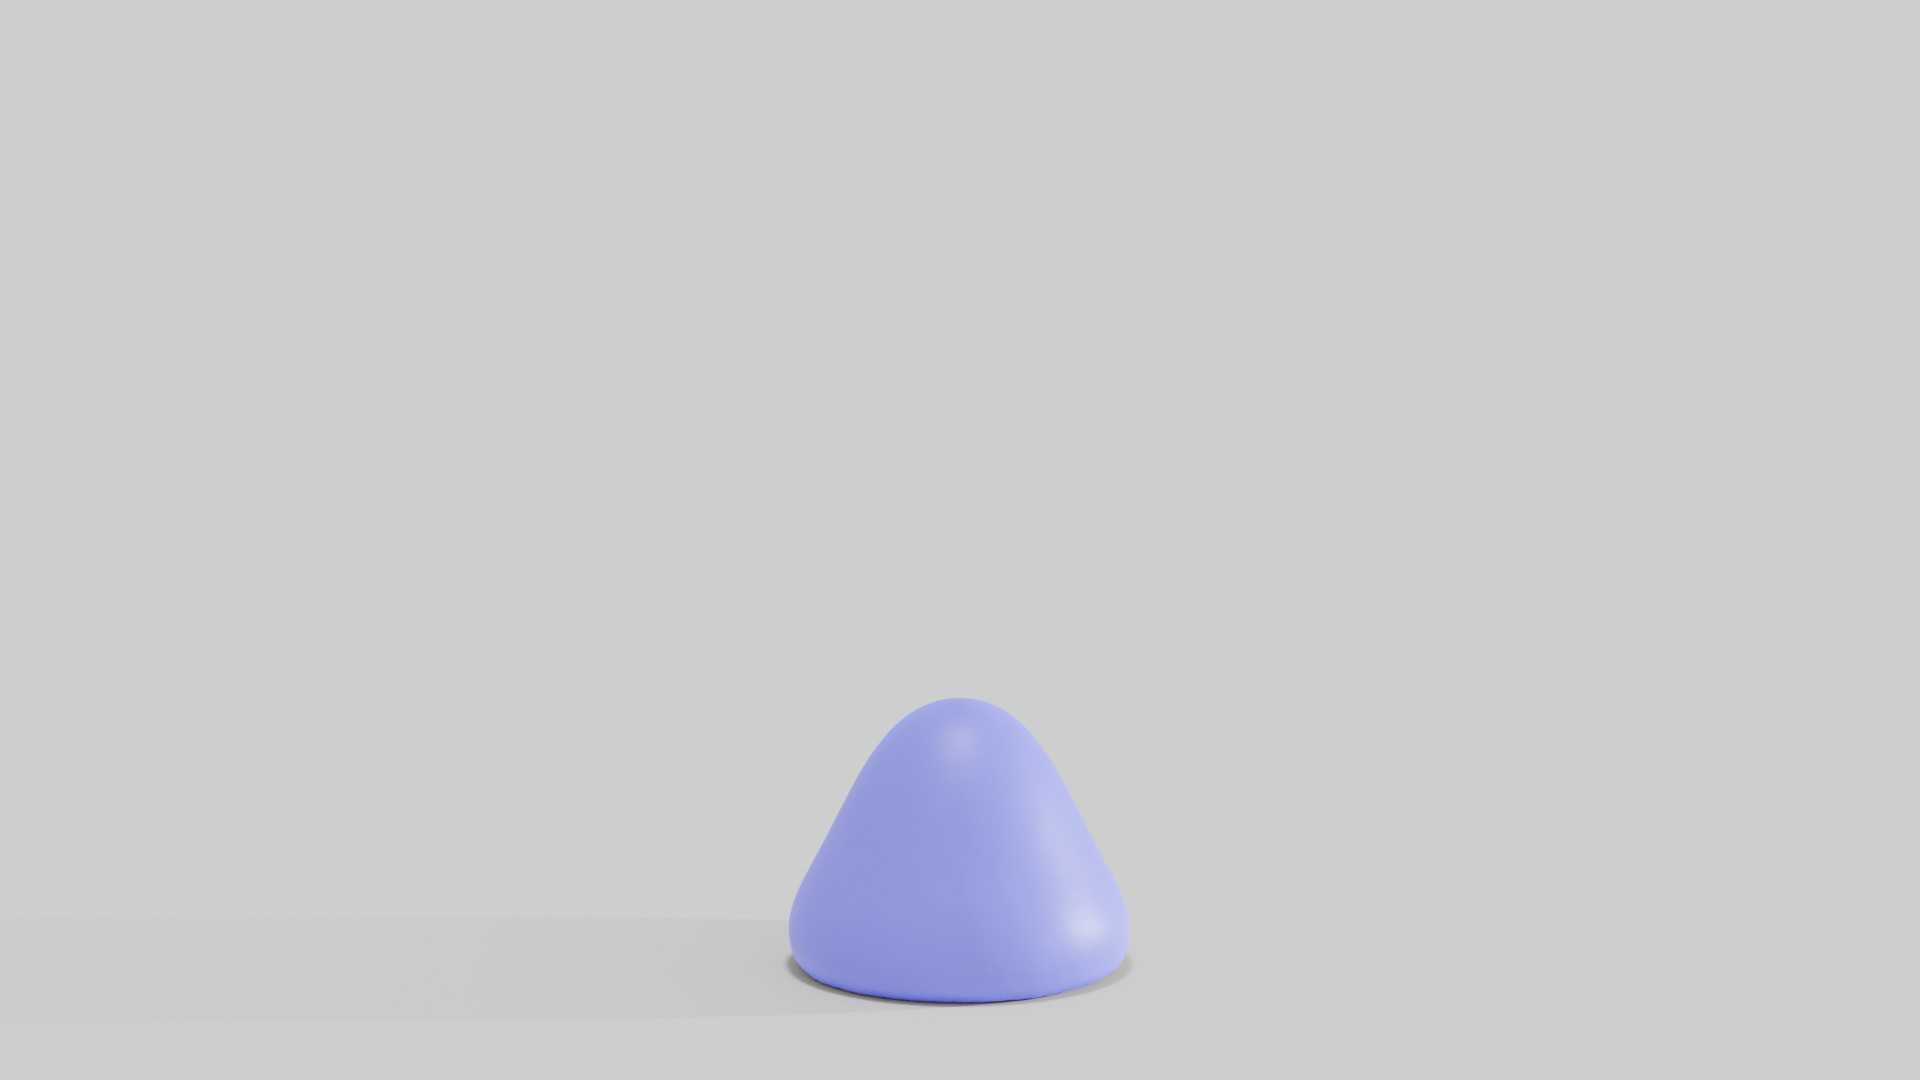
\includegraphics[width=2.0\textwidth]{images/soft_ball/045/0400.jpg}}
		%\caption*{(a5)}
		\label{sfig:ball-045-5}
	\end{subfigure}%
	\begin{subfigure}{.16\linewidth}
		\centering
		\adjustbox{trim={.25\width} {.0\height} {.25\width} {.4\height},clip}%
		{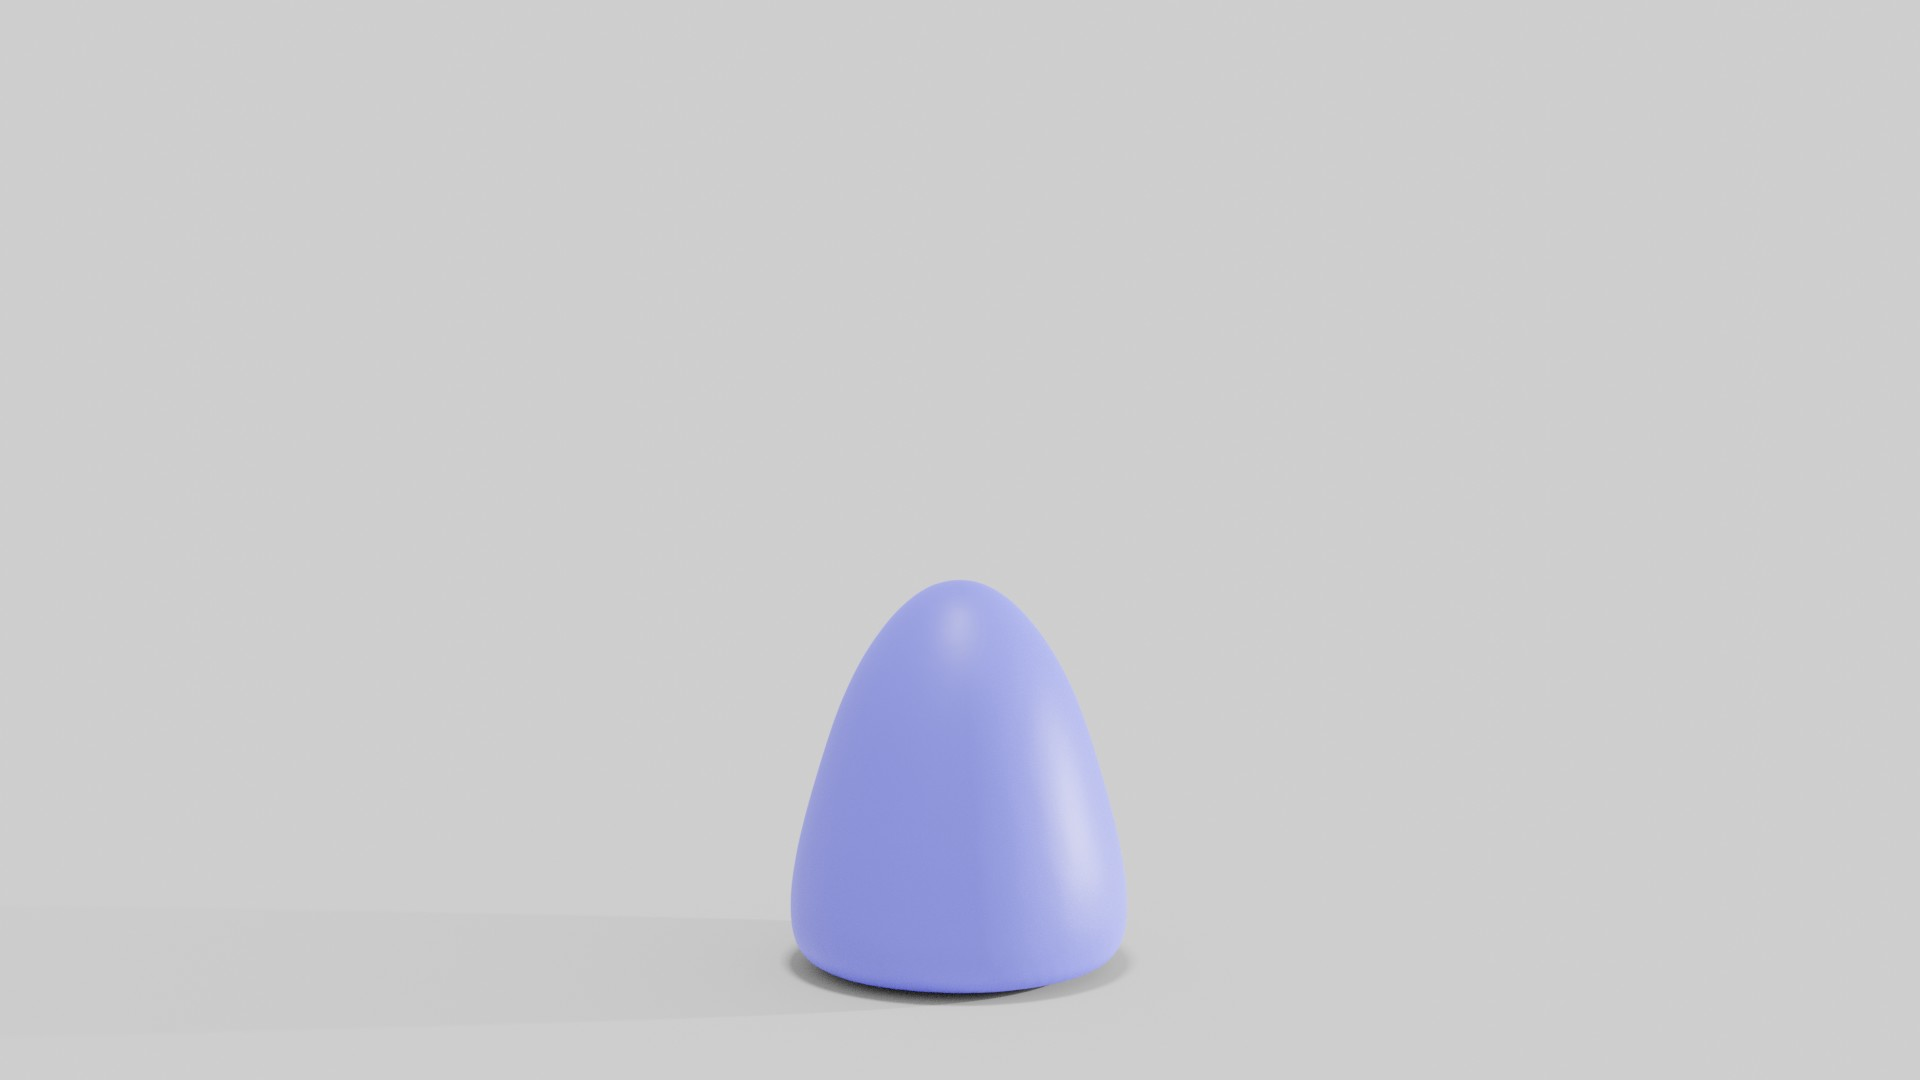
\includegraphics[width=2.0\textwidth]{images/soft_ball/045/0450.jpg}}
		%\caption*{(a6)}
		\label{sfig:ball-045-6}
	\end{subfigure}\hfill
	\begin{subfigure}{.03\linewidth}
		\rotatebox[origin=c]{90}{\footnotesize{\quad(b) UNH, $\nu=0.495$}}
	\end{subfigure}%
	\begin{subfigure}{.16\linewidth}
		\centering
		\adjustbox{trim={.25\width} {.0\height} {.25\width} {.4\height},clip}%
		{\includegraphics[width=2.0\textwidth]{images/soft_ball/0495/0200.jpg}}
		%\caption*{(a1)}
		\label{sfig:ball-0495-1}
	\end{subfigure}%
	\begin{subfigure}{.16\linewidth}
		\centering
		\adjustbox{trim={.25\width} {.0\height} {.25\width} {.4\height},clip}%
		{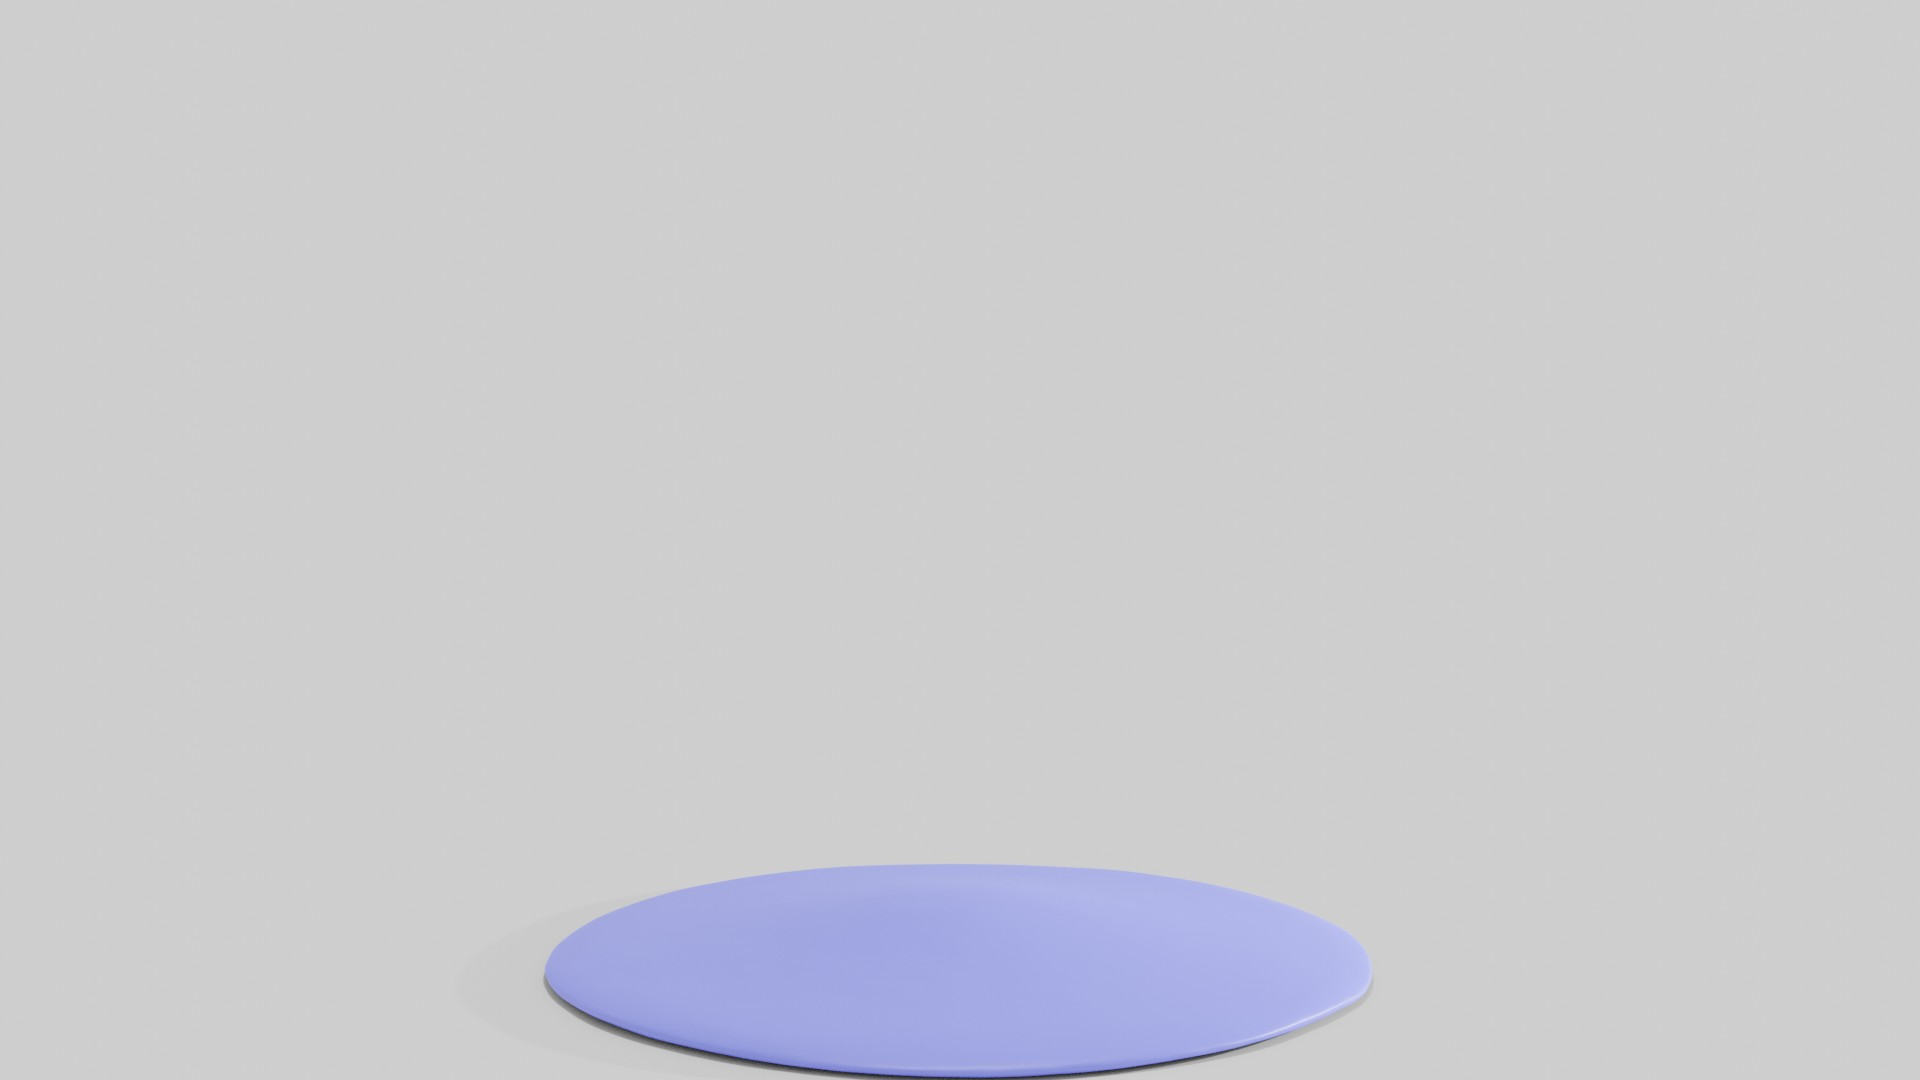
\includegraphics[width=2.0\textwidth]{images/soft_ball/0495/0250.jpg}}
		%\caption*{(a2)}
		\label{sfig:ball-0495-2}
	\end{subfigure}%
	\begin{subfigure}{.16\linewidth}
		\centering
		\adjustbox{trim={.25\width} {.0\height} {.25\width} {.4\height},clip}%
		{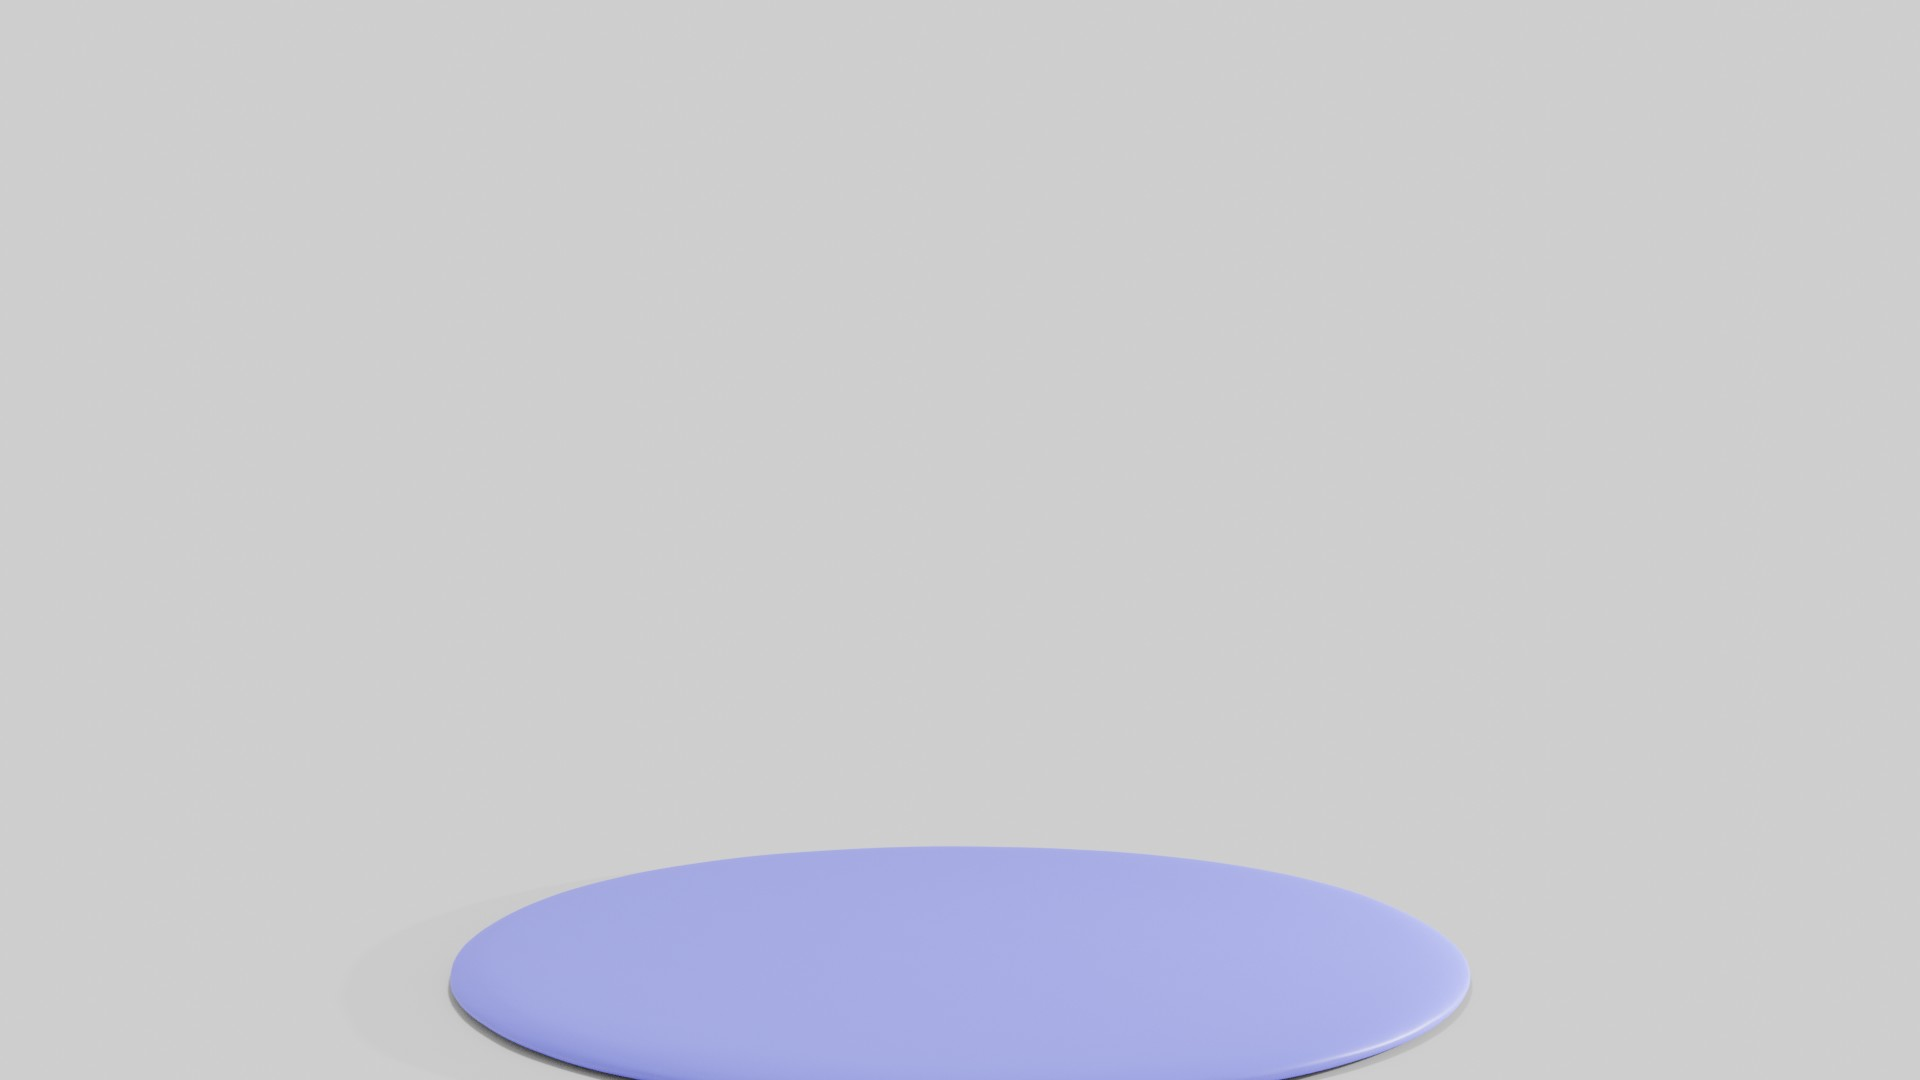
\includegraphics[width=2.0\textwidth]{images/soft_ball/0495/0300.jpg}}
		%\caption*{(a3)}
		\label{sfig:ball-0495-3}
	\end{subfigure}%
	\begin{subfigure}{.16\linewidth}
		\centering
		\adjustbox{trim={.25\width} {.0\height} {.25\width} {.4\height},clip}%
		{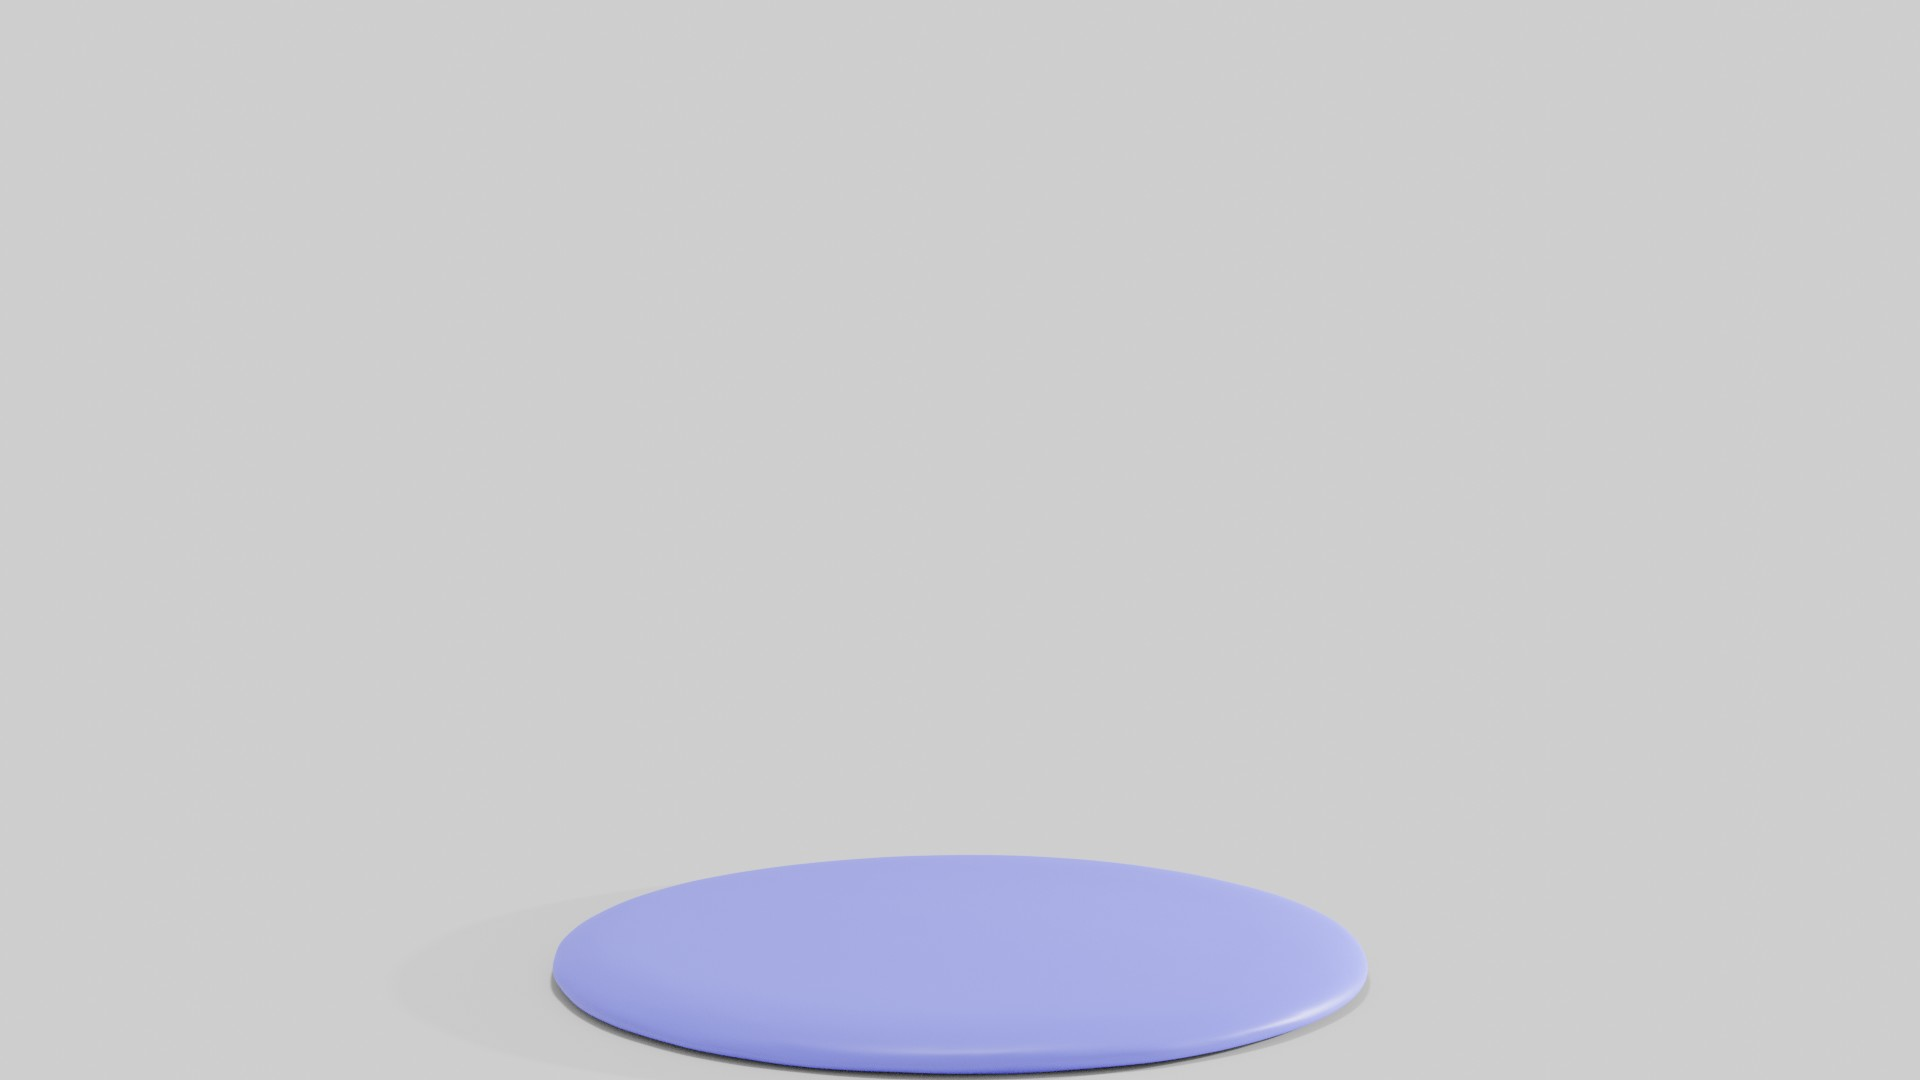
\includegraphics[width=2.0\textwidth]{images/soft_ball/0495/0350.jpg}}
		%\caption*{(a4)}
		\label{sfig:ball-0495-4}
	\end{subfigure}%
	\begin{subfigure}{.16\linewidth}
		\centering
		\adjustbox{trim={.25\width} {.0\height} {.25\width} {.4\height},clip}%
		{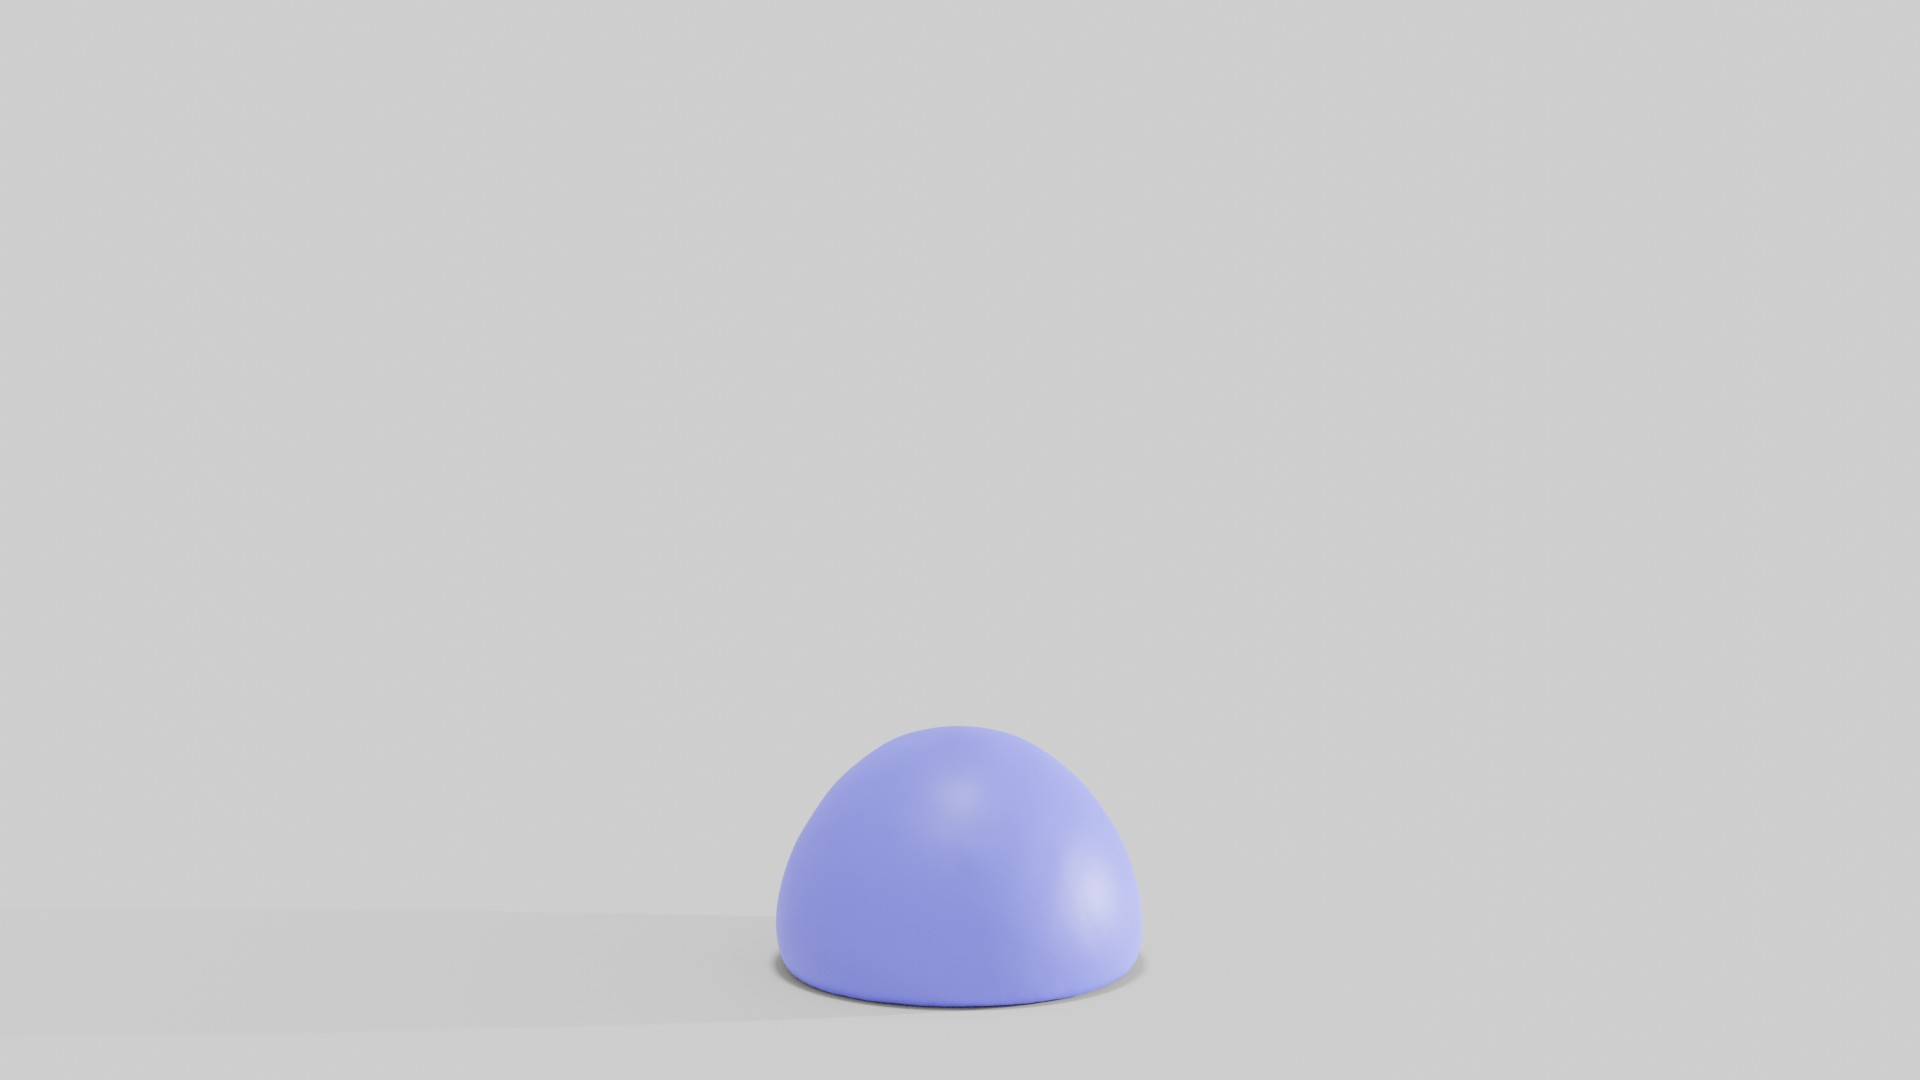
\includegraphics[width=2.0\textwidth]{images/soft_ball/0495/0400.jpg}}
		%\caption*{(a5)}
		\label{sfig:ball-0495-5}
	\end{subfigure}%
	\begin{subfigure}{.16\linewidth}
		\centering
		\adjustbox{trim={.25\width} {.0\height} {.25\width} {.4\height},clip}%
		{\includegraphics[width=2.0\textwidth]{images/soft_ball/0495/0450.jpg}}
		%\caption*{(a6)}
		\label{sfig:ball-0495-6}
	\end{subfigure}\hfill
	\begin{subfigure}{.03\linewidth}
		\rotatebox[origin=c]{90}{\footnotesize{\quad(c) Ours}}
	\end{subfigure}%
	\begin{subfigure}{.16\linewidth}
		\centering
		\adjustbox{trim={.25\width} {.0\height} {.25\width} {.4\height},clip}%
		{\includegraphics[width=2.0\textwidth]{images/soft_ball/vp/0200.jpg}}
		%\caption*{(a1)}
		\label{sfig:ball-vc-1}
	\end{subfigure}%
	\begin{subfigure}{.16\linewidth}
		\centering
		\adjustbox{trim={.25\width} {.0\height} {.25\width} {.4\height},clip}%
		{\includegraphics[width=2.0\textwidth]{images/soft_ball/vp/0250.jpg}}
		%\caption*{(a2)}
		\label{sfig:ball-vc-2}
	\end{subfigure}%
	\begin{subfigure}{.16\linewidth}
		\centering
		\adjustbox{trim={.25\width} {.0\height} {.25\width} {.4\height},clip}%
		{\includegraphics[width=2.0\textwidth]{images/soft_ball/vp/0300.jpg}}
		%\caption*{(a3)}
		\label{sfig:ball-vc-3}
	\end{subfigure}%
	\begin{subfigure}{.16\linewidth}
		\centering
		\adjustbox{trim={.25\width} {.0\height} {.25\width} {.4\height},clip}%
		{\includegraphics[width=2.0\textwidth]{images/soft_ball/vp/0350.jpg}}
		%\caption*{(a4)}
		\label{sfig:ball-vc-4}
	\end{subfigure}%
	\begin{subfigure}{.16\linewidth}
		\centering
		\adjustbox{trim={.25\width} {.0\height} {.25\width} {.4\height},clip}%
		{\includegraphics[width=2.0\textwidth]{images/soft_ball/vp/0400.jpg}}
		%\caption*{(a5)}
		\label{sfig:ball-vc-5}
	\end{subfigure}%
	\begin{subfigure}{.16\linewidth}
		\centering
		\adjustbox{trim={.25\width} {.0\height} {.25\width} {.4\height},clip}%
		{\includegraphics[width=2.0\textwidth]{images/soft_ball/vp/0450.jpg}}
		%\caption*{(a6)}
		\label{sfig:ball-vc-6}
	\end{subfigure}\hfill
	\begin{subfigure}{.03\linewidth}
		\rotatebox[origin=c]{90}{\footnotesize{\quad Frame}}
	\end{subfigure}%
	\begin{subfigure}{.16\linewidth}
		\centering
		200
	\end{subfigure}%
	\begin{subfigure}{.16\linewidth}
		\centering
		250
	\end{subfigure}%
	\begin{subfigure}{.16\linewidth}
		\centering
		300
	\end{subfigure}%
	\begin{subfigure}{.16\linewidth}
		\centering
		350
	\end{subfigure}%
	\begin{subfigure}{.16\linewidth}
		\centering
		400
	\end{subfigure}%
	\begin{subfigure}{.16\linewidth}
		\centering
		450
	\end{subfigure}%
	\caption{\textbf{Ball Drop}: An elastic sphere consisting of 64K tets is dropped to the ground. (a) shows the result with the standard UNH model with per-tet Poisson's ratio $\nu = 0.45$, where the ball loses more than half its volume in the second column. (b) is the UNH result with $\nu = 0.495$, where the volumetric locking makes the ball appear unnaturally stiff. Notice how the ball always retains its spherical shape and just get flattened and stretched in the vertical direction. (c) is the result using our CNH model with global volume constraint and local compression penalty with $\lambda$ equivalent to $\nu = 0.45$. Note that the volume of the sphere is preserved, producing a nice ``squash-and-stretch'' effect, and the artificial stiffness is removed.} \label{fig:fine-ball}
\end{figure}

We test a simple dynamic result of a soft ball consisting of 64K tets dropped under gravity and dropped to the ground in Figure~\ref{fig:fine-ball}. We used a timestep of 1ms and $\mu = 16.0$ KPa. Using a per-tet Poisson's ratio $\nu = 0.495$ results in the sphere behaving much stiffer than what the material parameters would suggest, while still losing up to 12.7\% of its volume. When using a per-tet Poisson's ratio of $\nu = 0.45$, the ball retains its appearance of soft elastic deformation, but loses up to 51\% of its original volume. Using our method, we are able to simulate the soft elastic deformations while preserving the volume down to solver accuracy, while being 5.7\% faster than the high Poisson's ratio case and only 3.7\% slower than the $\nu=0.45$ case. 


\section{Resolution Consistency}

\begin{figure}
	\centering
	\begin{subfigure}{.03\linewidth}
		\rotatebox[origin=c]{90}{\footnotesize{\quad(a) UNH, $\nu=0.45$}}
	\end{subfigure}%
	\begin{subfigure}{.16\linewidth}
		\centering
		\adjustbox{trim={.25\width} {.0\height} {.25\width} {.4\height},clip}%
		{\includegraphics[width=2.0\textwidth]{images/coarse_ball/045/0200.jpg}}
		%\caption*{(a1)}
		\label{sfig:ball-045-1}
	\end{subfigure}%
	\begin{subfigure}{.16\linewidth}
		\centering
		\adjustbox{trim={.25\width} {.0\height} {.25\width} {.4\height},clip}%
		{\includegraphics[width=2.0\textwidth]{images/coarse_ball/045/0250.jpg}}
		%\caption*{(a2)}
		\label{sfig:ball-045-2}
	\end{subfigure}%
	\begin{subfigure}{.16\linewidth}
		\centering
		\adjustbox{trim={.25\width} {.0\height} {.25\width} {.4\height},clip}%
		{\includegraphics[width=2.0\textwidth]{images/coarse_ball/045/0300.jpg}}
		%\caption*{(a3)}
		\label{sfig:ball-045-3}
	\end{subfigure}%
	\begin{subfigure}{.16\linewidth}
		\centering
		\adjustbox{trim={.25\width} {.0\height} {.25\width} {.4\height},clip}%
		{\includegraphics[width=2.0\textwidth]{images/coarse_ball/045/0350.jpg}}
		%\caption*{(a4)}
		\label{sfig:ball-045-4}
	\end{subfigure}%
	\begin{subfigure}{.16\linewidth}
		\centering
		\adjustbox{trim={.25\width} {.0\height} {.25\width} {.4\height},clip}%
		{\includegraphics[width=2.0\textwidth]{images/coarse_ball/045/0400.jpg}}
		%\caption*{(a5)}
		\label{sfig:ball-045-5}
	\end{subfigure}%
	\begin{subfigure}{.16\linewidth}
		\centering
		\adjustbox{trim={.25\width} {.0\height} {.25\width} {.4\height},clip}%
		{\includegraphics[width=2.0\textwidth]{images/coarse_ball/045/0450.jpg}}
		%\caption*{(a6)}
		\label{sfig:ball-045-6}
	\end{subfigure}\hfill
	\begin{subfigure}{.03\linewidth}
		\rotatebox[origin=c]{90}{\footnotesize{\quad(b) UNH, $\nu=0.495$}}
	\end{subfigure}%
	\begin{subfigure}{.16\linewidth}
		\centering
		\adjustbox{trim={.25\width} {.0\height} {.25\width} {.4\height},clip}%
		{\includegraphics[width=2.0\textwidth]{images/coarse_ball/0495/0200.jpg}}
		%\caption*{(a1)}
		\label{sfig:ball-0495-1}
	\end{subfigure}%
	\begin{subfigure}{.16\linewidth}
		\centering
		\adjustbox{trim={.25\width} {.0\height} {.25\width} {.4\height},clip}%
		{\includegraphics[width=2.0\textwidth]{images/coarse_ball/0495/0250.jpg}}
		%\caption*{(a2)}
		\label{sfig:ball-0495-2}
	\end{subfigure}%
	\begin{subfigure}{.16\linewidth} \begin {tikzpicture}
		\node [opacity=0.5,inner sep=0pt,anchor=south west,cross out,draw=red] at (0,0) {\adjincludegraphics[trim={.25\width} {.0\height} {.25\width} {.4\height},width=1.0\textwidth,clip]{images/coarse_ball/0495/0275.jpg}};
		\end {tikzpicture}
		\label{sfig:ball-0495-3}
	\end{subfigure}
	\begin{subfigure}{.48\linewidth}
		\centering
		\textcolor{red}{\textbf{Simulation failed at the 275th frame.}}
	\end{subfigure}\hfill
	\begin{subfigure}{.03\linewidth}
		\rotatebox[origin=c]{90}{\footnotesize{\quad(c) Ours}}
	\end{subfigure}%
	\begin{subfigure}{.16\linewidth}
		\centering
		\adjustbox{trim={.25\width} {.0\height} {.25\width} {.4\height},clip}%
		{\includegraphics[width=2.0\textwidth]{images/coarse_ball/vp/0200.jpg}}
		%\caption*{(a1)}
		\label{sfig:ball-vc-1}
	\end{subfigure}%
	\begin{subfigure}{.16\linewidth}
		\centering
		\adjustbox{trim={.25\width} {.0\height} {.25\width} {.4\height},clip}%
		{\includegraphics[width=2.0\textwidth]{images/coarse_ball/vp/0250.jpg}}
		%\caption*{(a2)}
		\label{sfig:ball-vc-2}
	\end{subfigure}%
	\begin{subfigure}{.16\linewidth}
		\centering
		\adjustbox{trim={.25\width} {.0\height} {.25\width} {.4\height},clip}%
		{\includegraphics[width=2.0\textwidth]{images/coarse_ball/vp/0300.jpg}}
		%\caption*{(a3)}
		\label{sfig:ball-vc-3}
	\end{subfigure}%
	\begin{subfigure}{.16\linewidth}
		\centering
		\adjustbox{trim={.25\width} {.0\height} {.25\width} {.4\height},clip}%
		{\includegraphics[width=2.0\textwidth]{images/coarse_ball/vp/0350.jpg}}
		%\caption*{(a4)}
		\label{sfig:ball-vc-4}
	\end{subfigure}%
	\begin{subfigure}{.16\linewidth}
		\centering
		\adjustbox{trim={.25\width} {.0\height} {.25\width} {.4\height},clip}%
		{\includegraphics[width=2.0\textwidth]{images/coarse_ball/vp/0400.jpg}}
		%\caption*{(a5)}
		\label{sfig:ball-vc-5}
	\end{subfigure}%
	\begin{subfigure}{.16\linewidth}
		\centering
		\adjustbox{trim={.25\width} {.0\height} {.25\width} {.4\height},clip}%
		{\includegraphics[width=2.0\textwidth]{images/coarse_ball/vp/0450.jpg}}
		%\caption*{(a6)}
		\label{sfig:ball-vc-6}
	\end{subfigure}\hfill
	\begin{subfigure}{.03\linewidth}
		\rotatebox[origin=c]{90}{\footnotesize{\quad Frame}}
	\end{subfigure}%
	\begin{subfigure}{.16\linewidth}
		\centering
		200
	\end{subfigure}%
	\begin{subfigure}{.16\linewidth}
		\centering
		250
	\end{subfigure}%
	\begin{subfigure}{.16\linewidth}
		\centering
		300
	\end{subfigure}%
	\begin{subfigure}{.16\linewidth}
		\centering
		350
	\end{subfigure}%
	\begin{subfigure}{.16\linewidth}
		\centering
		400
	\end{subfigure}%
	\begin{subfigure}{.16\linewidth}
		\centering
		450
	\end{subfigure}%
	\caption{\textbf{Coarse ball}: Similarly to Figure~\ref{fig:fine-ball}, a much coarser sphere with 4.7K tets is dropped to the ground. (a) shows the UNH result  with $\nu = 0.45$, where the ball has lost 52\% of its original volume at the 250th Frame, but gain 36\% volume at the 300th frame. (b) is the result of using UNH with $\nu = 0.495$, where due to using a coarser mesh the issue of locking is exacerbated, and the simulation fails to converge at the 275th frame. (c) is our result, where the simulation is stable and consistent with the result when using a much finer mesh, demonstrating our advantage of resolution consistency. } \label{fig:coarse-ball}
\end{figure}

An important advantage of enforcing volume preservation with zonal constraints is that it allows a way of simulating incompressible
objects using a much coarser mesh than by using a traditional 1-field method. C\'ea's lemma already couples the quasi-best approximation error 
with mesh resolution, and since a 1-field FE solutions also couple the bulk modulus to the upper bound of the approximation error, it makes it 
even harder to use a coarser mesh when bulk modulus is high. However, when incompressibility is decoupled from the bulk modulus, and we can 
use much smaller $\lambda$, we are able to achieve simulation results of a fine-mesh simulation that is consistent with a much coarser mesh. 
	%Figure~\ref{fig:fine-ball} shows a simple dynamic simulation with a very fine mesh, and Figure~\ref{fig:coarse-ball} shows the same simulation
	%using a much coarser mesh. We see that both the low Poisson ratio and our method achieves consistent visual results between the fine and coarse
	%case, but the high Poisson ratio case fails to converge very early in the simulation.


When a coarser mesh (~4.7K tets) is used, the advantage of our method becomes even clearer to see. For the low Poisson's ratio example, the maximum volume loss is almost equal to when using a finer mesh (~52.8\%). But after its impact with the ground, the ball actually gains volume due to the severe volumetric deformations resulting in extremely high volumetric elastic force, and the ball gains up to 36.1\% of its initial volume. The high Poisson's ratio case fails to converge after the 275th frame ( corresponds to the 0.275th second). This failure to converge when using a coarse mesh demonstrates how locking is aggravated when the simulation mesh is coarser, leading to a extremely high approximation error as predicted by C\'ea's Lemma. However, using our method allows a simulation of a completely volume preserving soft elastic ball even with a very coarse mesh. The visual result is consistent with when finer resolution was used, demonstrating that our method allows a resolution-consistent simulation of volume preserving soft objects. 

\section{Squeezing Armadillo}

\begin{figure}
	\centering
	\begin{subfigure}{.49\linewidth}
		\centering
		\adjustbox{trim={.10\width} {.0\height} {.15\width} {.0\height},clip}%
		{\includegraphics[width=3.3in]{images/armadillo/pr0495_mesh.png}}
		\label{sfig:armadillo_pr_0495}
	\end{subfigure}%
	\begin{subfigure}{.49\linewidth}
		\centering
		\adjustbox{trim={.10\width} {.0\height} {.15\width} {.0\height},clip}%
		{\includegraphics[width=3.3in]{images/armadillo/vc_mesh.png}}
		\label{sfig:armadillo_pr_0495}
	\end{subfigure} \par \medskip
	\begin{subfigure}{.49\linewidth}
		\centering
		\adjustbox{trim={.15\width} {.0\height} {.1\width} {.0\height},clip}%
		{\includegraphics[width=3.3in]{images/armadillo/pr0495.jpg}}
		\caption*{(a) UNH, $\nu = 0.495$}
		\label{sfig:armadillo_pr_0495}
	\end{subfigure}% 
	\begin{subfigure}{.49\linewidth}
		\centering
		\adjustbox{trim={.15\width} {.0\height} {.1\width} {.0\height},clip}%
		{\includegraphics[width=3.3in]{images/armadillo/vc.jpg}}
		\caption*{(b) Ours}
		\label{sfig:armadillo_ours}
	\end{subfigure}
	\caption{\textbf{Squeezing Armadillo}: An armadillo is squeezed between three cylinders. Two cylinders are placed under the armadillo and the top cylinder is moved down to almost touch the bottom cylinders. (a) and (b) shows the results at the most extreme deformation, top row visualized with the cylinder and the mesh topology, and the bottom row rendered without the cylinder. Using UNH with $\nu = 0.495$, the armadillo loses 15.11\% of its volume. Our method successfully preserves the entire volume of the armadillo, resulting in a much larger spread when completely deformed. The grid on the surface outlines the volume difference of the two deformed armadillos. }
	\label{fig:armadillo}
\end{figure}

To test the volume preservation and robustness of our method, we compress a 26K tet armadillo between two neighboring cylinders at the bottom and a moving cylinder at the top. The armadillo is divided into 6 zones: one for each arms and legs, the torso, and the entire body as a zone again. With Unconstrained Neo-Hookean $\nu = 0.495$, the armadillo loses up to 15.11\% of its volume even with such a high Poisson ratio. When the top cylinder moves down enough to almost touch the bottom cylinders, the volume lost on the armadillo's body is not recovered and does not flow much outside of the region between the cylinders, and as a result the body of the armadillo is completely flattened. However, using our method with $\lambda = 60, \beta = 12$, we are able to preserve the volume of the armadillo completely. Notice the bulging around the edges of the armadillo's body, where the volume lost in the compressed areas are gathered. The visual difference in volume preservation can be seen in Figure~\ref{fig:armadillo} where the grid outlines the area the squeezed armadillo covers.

\section{Leggings Fitting}

\begin{figure}
	\centering
	\includegraphics[width=1.0\textwidth]{images/teaser.png}
	\caption{\textbf{Leggigs fitting}: 
		Naively using $\nu = 0.4545$ produces qualitatively
		reasonable deformation, but the body loses a significant amount
		($\sim$19\%) of its volume, mostly in regions of high compression
		(see (b), and close-ups (e,h)). Using $\nu = 0.499$ preserves body
		volume up to an error of 0.5\%, but produces limited deformations
		due to locking (c,f,i).  By contrast, in our ``Constrained
		Neo-Hookean'' (CNH) method, we can designate volume preserving
		zones to match anatomical compartments, and exactly conserve
		volume within each zone while avoiding problems with volumetric
		locking. This results in more realistic displacement of soft
		tissues (d,g,j).
		\\
		In addition to visual differences, volume preservation can lead to
		significant differences in the predictions of how well the garment
		fits; UNH with $\nu = 0.4545$ predicts a waistband circumference 7
		cm smaller than that with $\nu = 0.499$, and 4.5cm smaller than
		with our method.  Our results can improve predictions of human
		soft tissue mechanics in applications ranging from virtual try-ons
		to visual effects.  }
	\label{fig:teaser}
\end{figure}

We apply our method on a cloth fitting example as shown in Figure~\ref{fig:teaser}. The goal of this
application is to predict fit of a tight fitting garment on a human subject. In this particular case
a pair of leggings are fit onto a female subject. Because human flesh is largely volume preserving, our
method is particularly suited for this example. We find that our method predicts a significantly
different fit than an Unconstrained Neo-Hookean model with a large Poisson's ratio.  This type of
simulation is used to determine general aesthetic fit as well as comfort, which can be used to
enhance the garment prototyping process.



\begin{table}[]
	\centering
	\begin{tabular}{@{}rcccccccc@{}}
		\toprule
		Example & Model & VC & $\lambda$ & $\beta$ & $\lambda_e$ & $t_r$ & $ i_{\textbf{avg}}$ \\
		\midrule
		Cloth-Body & SNH & no & 400.0 &  & 0.0 & 12.10 & 21.32 \\
		Cloth-Body & SNH & no & 40.0 &  & 0.0 & 12.93 & 23.09 \\
		Cloth-Body & Ours & yes & 120.0 & 6.0 & 0.0 & 12.82 & 17.98 \\
		Cloth-Body & Ours & yes & 120.0 & 6.0 &  100.0 & 14.63 & 19.18 \\
		\midrule
		Puck & SNH & no & 40.0 &   & 0.0 & 1.55 & 3.00 \\
		Puck & SNH & no & 400.0 &   & 0.0 & 1.58 & 3.14 \\
		Puck & Ours & yes & 100.0 & 0.0 & 0.0 & 2.25 & 4.00 \\
		Puck & Ours & yes & 100.0 & 9.0 & 0.0 & 1.93 & 3.38 \\
		Puck & Ours & yes & 100.0 & 9.0 & 100.0 & 2.25 & 3.51 \\
		\midrule
		Suspend & SNH & no & 400.0 & & 0.0 & 1.02 & 7.28 \\
		Suspend & Ours & yes & 40.0 & 0.0 &  & 1.02 & 6.52 \\
		\midrule
		Stretch & SNH & no & 40.0 & & 0.0 & 2.80 & 4.51 \\
		Stretch & SNH & no & 400.0 & & 0.0 & 9.91 & 14.33 \\
		Stretch & Ours & yes & 25.0 & 0.0 & 0.0 & 7.89 & 9.92 \\
		Stretch & Ours & yes & 25.0 & 1.0 & 0.0 & 7.28 & 9.24 \\
		Stretch & Ours & yes & 25.0 & 1.0 & 10.0 & 6.25 & 7.33 \\
		\midrule
		Twist & SNH & no & 100.0 & & 0.0 & 86.06 & 138.33 \\
		Twist & Ours & no & 100.0 & 9.0 & 0.0 & 37.32 & 50.33 \\
		Twist & Ours & yes & 100.0 & 6.0 & 0.0 & 62.15 & 90.33 \\
		Twist & Ours & yes & 100.0 & 6.0 &  15.0  & 103.10 & 92 \\
		\midrule
		Ball (Fine) & NH & no & 120.0 & & 0.0 & 17.27 & 14.64 \\
		Ball (Fine) & NH & no & 400.0 & & 0.0 & 19.00 & 15.90 \\
		Ball (Fine) & Ours & yes & 120.0 & 1.0 & 0.0 & 17.91 & 12.29 \\
		Ball (Coarse) & NH & no & 120.0 & & 0.0 & 1.81 & 15.08 \\
		Ball (Coarse) & NH & no & 400.0 & & 0.0 & 2.50 & 21.84 \\
		Ball (Coarse) & Ours & yes & 120.0 & 1.0 & 0.0 & 2.71 & 22.10 \\
		\midrule
		Armadillo & SNH & no & 400.0 & & 40.0 & 6.26 & 11.29 \\
		Armadillo & Ours & yes & 60.0 & 12.0 & 40.0 & 6.97 & 10.84 \\
		\bottomrule
	\end{tabular}%
	\caption{\textbf{Performance Analysis}: Performance table representing average run times per frame, and average Ipopt iterations per frame for major examples. SNH is the Stable Neo-Hookean
		% \eqref{e-snh}
		\cite{Smith:2018}. (VC: Volume Constraint, $t_r$: Run Times per Frame (sec.), $i_{\textbf{avg}}$: Avg. Ipopt Iterations.)}
	\label{tab:performance}
\end{table}
\chapter{Conclusion}
\label{ch:Conclusion}

Although our method generates more realistic volume preservation and
reduces locking, for simulations without large deformations, the
standard Neo-Hookean model may be sufficient due to its
simplicity. This is especially true when no other constraints, such as due to external contact, are present in the simulation. Constrained optimization adds
some complexity to the simulation, though our results in Table
\ref{tab:performance} show that the increase is computation times is
not prohibitive in most cases. Overall, our findings allow a simple and inexpensive
extension to existing FEM systems to solve the problem of volumetric
locking while simulating incompressible materials such as the human
body.

\paragraph{Performance} Our formulation uses exact non-linear volume constraints on a non-linear
optimization problem to preserve volume exactly in demanding applications like statics and dynamics
with large time steps.  This limits the choice of optimization solvers to ones that
support non-linear equality constraints (e.g. Interior Point or SQP solvers).  However, for dynamics problems
with smaller time steps, or in applications with tolerance for volume loss/gain, we recommend
linearizing the volume constraint, which drastically simplifies the problem. This can reduce the
overhead of enforcing equality constraints, while still avoiding locking.

\paragraph{Choosing $\lambda$} By decoupling $\lambda$ from its physical meaning, our formulation is
faced with an additional challenge, which is to determine how exactly $\lambda$ effects the outcome
of a simulation.  Fortunately, this is not a significant drawback since material parameters for
standard Neo-Hookean FEM simulations also deviate from their measured values due to numerical
stiffenning. This means that even the parameters of standard models require manual tuning to
reproduce real phenomena in simulation.  Luckily data-driven methods for determining simulation
parameters (which has seen significant attention in recent literature) are generally agnostic to the
true physical meaning of these parameters, and thus are equally as compatible with our method.

In conclusion, we presented a general method for realistic volumetric FEM simulations of human tissue.
Our method provides exact volume preservation without the artificial stiffness due to volumetric
locking using zonal volume constraints. This method gives artists the ability to define volume
preserving zones that conform to anatomical compartments and automatically produces
``squash-and-stretch'' effects. In addition, we introduced an epidermis model for simulating
skin dynamics, as an additional surface area-preserving potential. We also proposed a
modification to the energy potential to provide control over local volume flow
that results in improved
recovery during extreme compression and inversion. Our approach can be applied to a variety of energy
models. In particular, we have demonstrated the effectiveness of these simple modifications to the
invariant based non-linear hyperelastic energies like the Neo-Hookean and Stable Neo-Hookean energy
models.


%    3. Notes
%    4. Footnotes

%    5. Bibliography
\begin{singlespace}
\raggedright
\bibliographystyle{abbrvnat}
\bibliography{biblio}
\end{singlespace}

\appendix
%    6. Appendices (including copies of all required UBC Research
%       Ethics Board's Certificates of Approval)
%\include{reb-coa}	% pdfpages is useful here
\chapter{Appendix}
\label{ap: Penalty}

Extending the idea of \eqref{eq:penalty_function}, one can devise a more highly nonlinear versions of the penalty functional. For example, from

\begin{equation}
\frac{\partial^2 U_2(J;\beta)}{\partial J^2} = \beta(J-1)^4 + 1,
\end{equation}

we can derive 
\begin{align}
\frac{\partial U_2(J;\beta)}{\partial J} &= \frac{1}{5} (J-1) \left[ \beta(J-1)^4 + 5 \right], and \\
U_2(J;\beta) &= \frac{1}{30} (J-1)^2 \left[ \beta (J-1)^4 + 15 \right].
\end{align}

In this sense, we can derive a penalty function of arbitrary order, based on the second derivative. To satisfy condition \textbf{e} from Section~\ref{ch:Volume Penalty}, the order of the second derivative must be an even number, so for a natural number $n$ one can define a second derivative as

\begin{equation}
\frac{\partial^2 U_n(J;\beta)}{\partial J^2} = \beta(J-1)^{2n} + 1,
\end{equation}

then build the penalty function $U_n(J; \beta)$ that satisfies all the five conditions from the second derivative as follows,

\begin{equation}
U_n(J;\beta) = \frac{1}{(2n+1)(2n+2)} (J-1)^2 \left[ \beta (J-1)^{2n} + \frac{(2n+1)(2n+2)}{2} \right].
\end{equation}

We plot the runtimes and average Ipopt iterations for the first few $n$ of these penalties, for the cube twist simulation in Figure~\ref{fig:penalty_comparison}, with $\beta = 1$.
Notice how the runtime and number of iterations increase linearly depending on $n$. 
From this simple experiment, we can conclude that although the added nonlinearity of the gradient is beneficial for resolving tet inversions, additional nonlinearity of the energy is actually harmful for the performance. Therefore, we argue that our choice of the penalty functional in \eqref{eq:penalty_function} is indeed optimal for our purposes.

\begin{figure}[t] 
	\centering
	\begin{subfigure}{.49\linewidth}
		\centering \includegraphics[width=2.5in]{images/penalty_runtimes.pdf}
		\caption*{(a)}
		\label{sfig:pen_runtimes}
	\end{subfigure}%
	\begin{subfigure}{.49\linewidth}
		\centering \includegraphics[width=2.5in]{images/penalty_iters.pdf}
		\caption*{(b)}
		\label{sfig:pen_iters}
	\end{subfigure}%
	\caption{\textbf{Penalty Function Performance}: A plot of penalty functions $U_n$ of different orders $n$ from 1 to 6. }
	\label{fig:penalty_comparison}
\end{figure}

\backmatter
%    7. Index
% See the makeindex package: the following page provides a quick overview
% <http://www.image.ufl.edu/help/latex/latex_indexes.shtml>


\end{document}
